\documentclass[]{book}
\usepackage{lmodern}
\usepackage{amssymb,amsmath}
\usepackage{ifxetex,ifluatex}
\usepackage{fixltx2e} % provides \textsubscript
\ifnum 0\ifxetex 1\fi\ifluatex 1\fi=0 % if pdftex
  \usepackage[T1]{fontenc}
  \usepackage[utf8]{inputenc}
\else % if luatex or xelatex
  \ifxetex
    \usepackage{mathspec}
  \else
    \usepackage{fontspec}
  \fi
  \defaultfontfeatures{Ligatures=TeX,Scale=MatchLowercase}
\fi
% use upquote if available, for straight quotes in verbatim environments
\IfFileExists{upquote.sty}{\usepackage{upquote}}{}
% use microtype if available
\IfFileExists{microtype.sty}{%
\usepackage{microtype}
\UseMicrotypeSet[protrusion]{basicmath} % disable protrusion for tt fonts
}{}
\usepackage{hyperref}
\hypersetup{unicode=true,
            pdftitle={Estadística para Ciencias Sociales con R},
            pdfauthor={Eduardo Bologna},
            pdfborder={0 0 0},
            breaklinks=true}
\urlstyle{same}  % don't use monospace font for urls
\usepackage{natbib}
\bibliographystyle{apalike}
\usepackage{color}
\usepackage{fancyvrb}
\newcommand{\VerbBar}{|}
\newcommand{\VERB}{\Verb[commandchars=\\\{\}]}
\DefineVerbatimEnvironment{Highlighting}{Verbatim}{commandchars=\\\{\}}
% Add ',fontsize=\small' for more characters per line
\usepackage{framed}
\definecolor{shadecolor}{RGB}{248,248,248}
\newenvironment{Shaded}{\begin{snugshade}}{\end{snugshade}}
\newcommand{\AlertTok}[1]{\textcolor[rgb]{0.94,0.16,0.16}{#1}}
\newcommand{\AnnotationTok}[1]{\textcolor[rgb]{0.56,0.35,0.01}{\textbf{\textit{#1}}}}
\newcommand{\AttributeTok}[1]{\textcolor[rgb]{0.77,0.63,0.00}{#1}}
\newcommand{\BaseNTok}[1]{\textcolor[rgb]{0.00,0.00,0.81}{#1}}
\newcommand{\BuiltInTok}[1]{#1}
\newcommand{\CharTok}[1]{\textcolor[rgb]{0.31,0.60,0.02}{#1}}
\newcommand{\CommentTok}[1]{\textcolor[rgb]{0.56,0.35,0.01}{\textit{#1}}}
\newcommand{\CommentVarTok}[1]{\textcolor[rgb]{0.56,0.35,0.01}{\textbf{\textit{#1}}}}
\newcommand{\ConstantTok}[1]{\textcolor[rgb]{0.00,0.00,0.00}{#1}}
\newcommand{\ControlFlowTok}[1]{\textcolor[rgb]{0.13,0.29,0.53}{\textbf{#1}}}
\newcommand{\DataTypeTok}[1]{\textcolor[rgb]{0.13,0.29,0.53}{#1}}
\newcommand{\DecValTok}[1]{\textcolor[rgb]{0.00,0.00,0.81}{#1}}
\newcommand{\DocumentationTok}[1]{\textcolor[rgb]{0.56,0.35,0.01}{\textbf{\textit{#1}}}}
\newcommand{\ErrorTok}[1]{\textcolor[rgb]{0.64,0.00,0.00}{\textbf{#1}}}
\newcommand{\ExtensionTok}[1]{#1}
\newcommand{\FloatTok}[1]{\textcolor[rgb]{0.00,0.00,0.81}{#1}}
\newcommand{\FunctionTok}[1]{\textcolor[rgb]{0.00,0.00,0.00}{#1}}
\newcommand{\ImportTok}[1]{#1}
\newcommand{\InformationTok}[1]{\textcolor[rgb]{0.56,0.35,0.01}{\textbf{\textit{#1}}}}
\newcommand{\KeywordTok}[1]{\textcolor[rgb]{0.13,0.29,0.53}{\textbf{#1}}}
\newcommand{\NormalTok}[1]{#1}
\newcommand{\OperatorTok}[1]{\textcolor[rgb]{0.81,0.36,0.00}{\textbf{#1}}}
\newcommand{\OtherTok}[1]{\textcolor[rgb]{0.56,0.35,0.01}{#1}}
\newcommand{\PreprocessorTok}[1]{\textcolor[rgb]{0.56,0.35,0.01}{\textit{#1}}}
\newcommand{\RegionMarkerTok}[1]{#1}
\newcommand{\SpecialCharTok}[1]{\textcolor[rgb]{0.00,0.00,0.00}{#1}}
\newcommand{\SpecialStringTok}[1]{\textcolor[rgb]{0.31,0.60,0.02}{#1}}
\newcommand{\StringTok}[1]{\textcolor[rgb]{0.31,0.60,0.02}{#1}}
\newcommand{\VariableTok}[1]{\textcolor[rgb]{0.00,0.00,0.00}{#1}}
\newcommand{\VerbatimStringTok}[1]{\textcolor[rgb]{0.31,0.60,0.02}{#1}}
\newcommand{\WarningTok}[1]{\textcolor[rgb]{0.56,0.35,0.01}{\textbf{\textit{#1}}}}
\usepackage{longtable,booktabs}
\usepackage{graphicx,grffile}
\makeatletter
\def\maxwidth{\ifdim\Gin@nat@width>\linewidth\linewidth\else\Gin@nat@width\fi}
\def\maxheight{\ifdim\Gin@nat@height>\textheight\textheight\else\Gin@nat@height\fi}
\makeatother
% Scale images if necessary, so that they will not overflow the page
% margins by default, and it is still possible to overwrite the defaults
% using explicit options in \includegraphics[width, height, ...]{}
\setkeys{Gin}{width=\maxwidth,height=\maxheight,keepaspectratio}
\IfFileExists{parskip.sty}{%
\usepackage{parskip}
}{% else
\setlength{\parindent}{0pt}
\setlength{\parskip}{6pt plus 2pt minus 1pt}
}
\setlength{\emergencystretch}{3em}  % prevent overfull lines
\providecommand{\tightlist}{%
  \setlength{\itemsep}{0pt}\setlength{\parskip}{0pt}}
\setcounter{secnumdepth}{5}
% Redefines (sub)paragraphs to behave more like sections
\ifx\paragraph\undefined\else
\let\oldparagraph\paragraph
\renewcommand{\paragraph}[1]{\oldparagraph{#1}\mbox{}}
\fi
\ifx\subparagraph\undefined\else
\let\oldsubparagraph\subparagraph
\renewcommand{\subparagraph}[1]{\oldsubparagraph{#1}\mbox{}}
\fi

%%% Use protect on footnotes to avoid problems with footnotes in titles
\let\rmarkdownfootnote\footnote%
\def\footnote{\protect\rmarkdownfootnote}

%%% Change title format to be more compact
\usepackage{titling}

% Create subtitle command for use in maketitle
\providecommand{\subtitle}[1]{
  \posttitle{
    \begin{center}\large#1\end{center}
    }
}

\setlength{\droptitle}{-2em}

  \title{Estadística para Ciencias Sociales con R}
    \pretitle{\vspace{\droptitle}\centering\huge}
  \posttitle{\par}
    \author{Eduardo Bologna}
    \preauthor{\centering\large\emph}
  \postauthor{\par}
      \predate{\centering\large\emph}
  \postdate{\par}
    \date{15 de julio de 2019}

\usepackage{booktabs}
\usepackage{amsthm}
\makeatletter
\def\thm@space@setup{%
  \thm@preskip=8pt plus 2pt minus 4pt
  \thm@postskip=\thm@preskip
}

\makeatother
\ifxetex
  \usepackage{polyglossia}
  \setmainlanguage{spanish}
  % Tabla en lugar de cuadro
  \gappto\captionsspanish{\renewcommand{\tablename}{Tabla}  
          \renewcommand{\listtablename}{Índice de tablas}}
\else
  \usepackage[spanish,es-tabla]{babel}
\fi

% For kableExtra
\usepackage{booktabs}
\usepackage{longtable}
\usepackage{array}
\usepackage{multirow}
\usepackage{wrapfig}
\usepackage{float}
\usepackage{colortbl}
\usepackage{pdflscape}
\usepackage{tabu}
\usepackage{threeparttable}
\usepackage{threeparttablex}
\usepackage[normalem]{ulem}
\usepackage{makecell}
\usepackage{xcolor}

\begin{document}
\maketitle

{
\setcounter{tocdepth}{1}
\tableofcontents
}
\hypertarget{los-datos-estadisticos}{%
\chapter{Los datos estadísticos}\label{los-datos-estadisticos}}

En este capítulo se desarrollan procedimientos para presentar la información de manera accesible para que pueda ser analizada y luego interpretada. Para poder extraer significado de los datos recogidos es necesario primero dedicar un esfuerzo a organizarlos, a presentarlos de manera comprensible, una operación previa a la aplicación de las técnicas de análisis que se verán más adelante.

La ciencia se interesa por la producción de conocimiento validado, uno de cuyos requisitos es que pueda ser comunicado de manera inequívoca, que se confronten las conclusiones a que llegan y los métodos que usan diferentes investigadores. Esto implica la necesidad de usar un lenguaje que permita el intercambio entre investigadores y que dependa, en el menor grado posible, de las impresiones subjetivas o de las interpretaciones que cada investigador individual dé a los conceptos. Se busca un vocabulario tan unívoco como sea posible. Un modo de acercarse a lograr esta comunicabilidad de las ideas, de los métodos y de los resultados, es definir, de la manera más precisa posible, los elementos acerca de los que se habla.

Alguna vez hemos dado con expresiones como ``esta persona es más inteligente que aquella''. ¿Qué se quiere decir exactamente con eso?, la afirmación podría provenir de algún evento en que se vio a esa persona actuando de manera que llamaríamos inteligente, aunque esto también puede confundirse con astucia: no es infrecuente usar el adjetivo inteligente para un estafador, alguien a quien le resulta fácil engañar a otros; y, a la inversa, sería poco inteligente quien se deja engañar con facilidad. O bien, a menudo decimos que alguien es inteligente porque obtiene buenos resultados en sus estudios. Esto es parte de la imprecisión en la definición de un concepto. Si se dispone de una definición de inteligencia, se puede saber cuándo aplicar esa idea a alguien, cuándo una conducta es inteligente, inclusive, cómo ayudar a desarrollar la inteligencia. Si se puede definir el concepto con el que se trabaja, se pueden indicar ciertas operaciones a realizar para evaluarlo y así conocer cuál es el nivel de inteligencia de un sujeto en particular.

Luego de definir el concepto con el que se trabaja, se requiere diseñar un instrumento que refleje esa definición y finalmente aplicar este instrumento a las personas que se evaluarán. Al hacer esto último se obtiene un resultado que, si se expresa de manera cuantitativa, permite hacer comparaciones del aspecto que representa ese concepto, entre personas, entre grupos, etc.

¿Pueden compararse personas? La respuesta es no, porque cada persona tiene una infinidad de aspectos que la caracterizan y la hacen única. Por el contrario lo que sí pueden compararse son características claramente definidas de las personas. Del mismo modo no se pueden comparar escuelas, ni hogares, ni países si no se especifica en qué aspecto se realiza la comparación. O dicho de otro modo, cuál es la característica que se compara, y cómo se mide esa característica.

Podemos decir que una persona tiene más escolarización formal que otra, indicando con eso que ha aprobado más años de la escuela o de la universidad. Podemos decir que un hogar es diferente a otro si uno se compone de una pareja sola y el otro incluye tres hijos. Un país puede tener más habitantes, un régimen político diferente, o mayor libertad de expresión que otro. En todos los casos especificamos una característica (un rasgo o un estado), sobre la base del cual hacemos la comparación.

\hypertarget{la-seleccion-de-la-informacion-pertinente}{%
\section{La selección de la información pertinente}\label{la-seleccion-de-la-informacion-pertinente}}

Cuando se ha decidido quienes son los sujetos de la observación; es decir, una vez que se sabe a quiénes se observará, deben elegirse ciertas características de esos sujetos para observar . Cada unidad que resulta de interés para la investigación tiene un conjunto muy grande de características observables y siempre se realiza una selección de esas características. Se trata de un recorte que permite comprender mejor ciertos aspectos, dejando de lado otros. La información que seleccionamos para observar se denomina pertinente para la investigación.

Cuando se decide cuál es la información pertinente, se la puede recabar de varios individuos y cambiar la óptica desde el caso particular a la regularidad colectiva. Es un cambio desde el individuo hacia el grupo. La siguiente es una lista que indica el área en que les gustaría trabajar cuando se reciban, a nueve estudiantes de primer año de Psicología:

\begin{longtable}[]{@{}lr@{}}
\caption{\label{tab:unnamed-chunk-2}Área de trabajo preferida.}\tabularnewline
\toprule
Alumno & Área\tabularnewline
\midrule
\endfirsthead
\toprule
Alumno & Área\tabularnewline
\midrule
\endhead
Susana & Clínica\tabularnewline
Marcos & Laboral\tabularnewline
Daniel & Clínica\tabularnewline
Federico & Social\tabularnewline
María & Clínica\tabularnewline
Pedro & Educacional\tabularnewline
Eugenia & Clínica\tabularnewline
Mabel & Educacional\tabularnewline
Francisco & Laboral\tabularnewline
\bottomrule
\end{longtable}

La lista los individualiza, los reconoce por su nombre, indica qué área le gustaría a cada uno y solo eso, no se sabe la edad de cada uno, ni sus intereses políticos ni el deporte favorito, solo se seleccionó como pertinente para este ejemplo, el área en que le gustaría trabajar. Si ahora se transforma esa lista en una tabla:

\begin{longtable}[]{@{}lr@{}}
\caption{\label{tab:unnamed-chunk-3}Área de trabajo preferida.}\tabularnewline
\toprule
Área & Casos\tabularnewline
\midrule
\endfirsthead
\toprule
Área & Casos\tabularnewline
\midrule
\endhead
Clínica & 4\tabularnewline
Educacional & 2\tabularnewline
Laboral & 2\tabularnewline
Social & 1\tabularnewline
\bottomrule
\end{longtable}

Se lee que Clínica es un área preferida por cuatro alumnos, Laboral y Educacional por dos y a Social solo la menciona uno. Las personas desaparecieron, ya no hay nombres, hemos abstraído para referirnos al área preferida, no a los alumnos. En la tabla se ve que lo más frecuente es que se prefiera Clínica, y que Social es poco frecuente. Se pasó de la lista de individuos a la tabla de valores. Nos despegamos de los casos a fin de buscar la regularidad en el conjunto. Más adelante diremos que se ha pasado de la matriz de datos a la distribución de frecuencias, que constituye una reducción o un primer resumen de la información disponible.

Consideremos el siguiente cuestionario, que se aplicó en 2019 a personas con edades 18 y 35 años.

\begin{figure}

{\centering 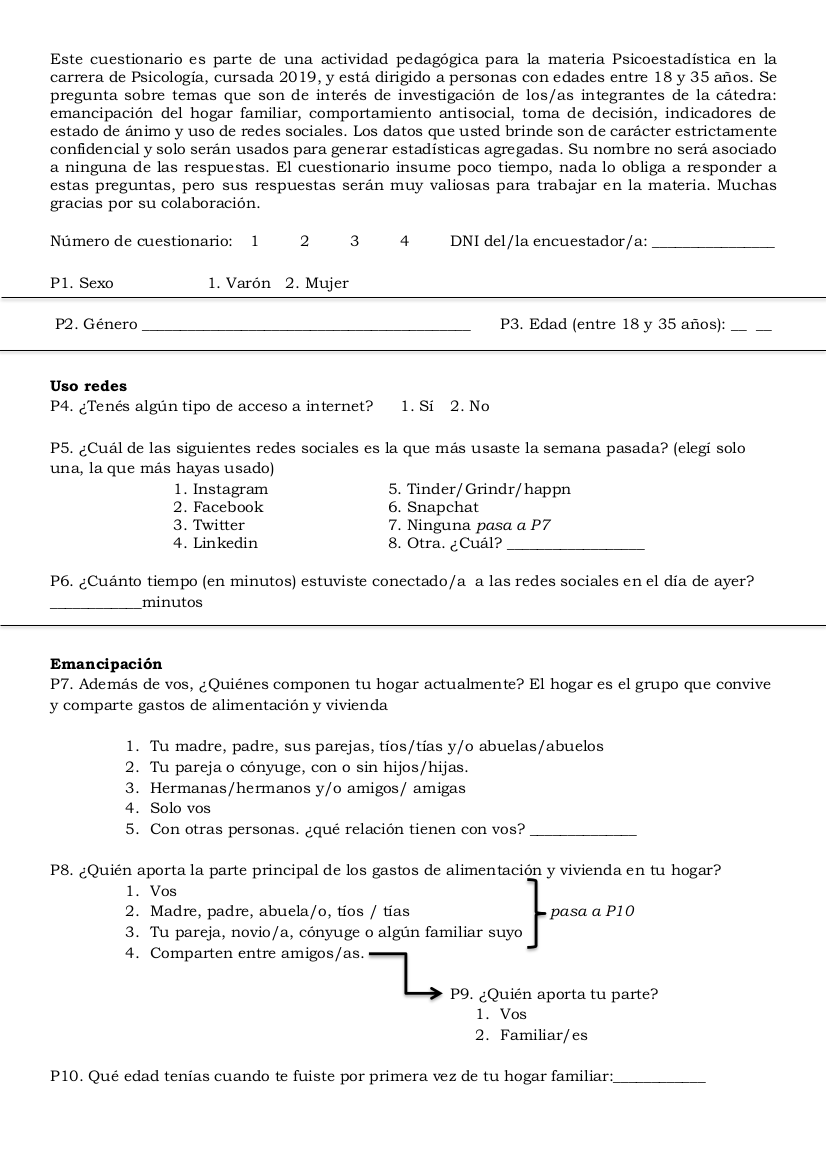
\includegraphics{imagenes/cuestionario2019_01} 

}

\caption{Cuestionario 2019}\label{fig:cuestionario}
\end{figure}
\begin{figure}

{\centering 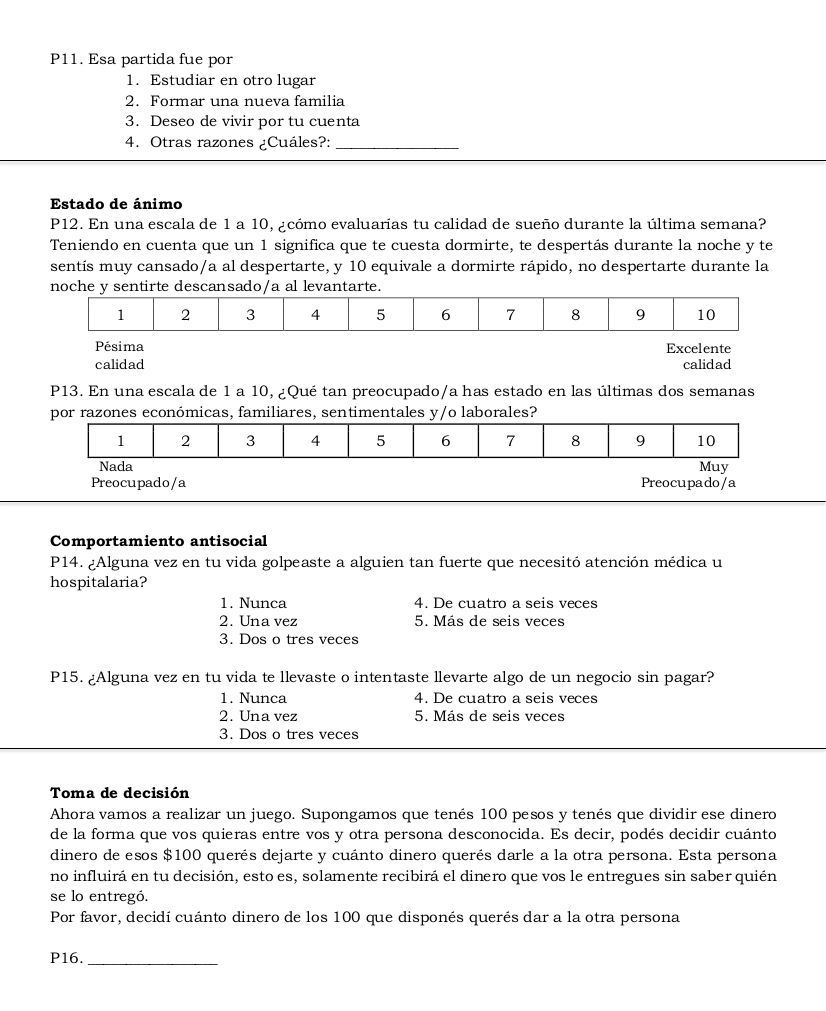
\includegraphics{imagenes/cuestionario2019_02} 

}

\caption{Cuestionario 2019}\label{fig:cuestionario}
\end{figure}

Este instrumento de producción de datos que es el cuestionario, se dirige a una población definida: personas entre 18 y 35 años. En él se solicita información sobre un conjunto seleccionado de características; los ítems numerados desde P1 hasta P16. Se trata de unos pocos aspectos de cada persona los que interesan para esta investigación; no se tiene en cuenta, por ejemplo la opinión política de quienes responden, ni su estatura o la región en que viven. Estas últimas y muchas más son características de estas personas, pero están fuera del alcance de la investigación. Esto muestra a qué nos referimos con que la información seleccionada constituye un recorte, es una parcialización de los individuos que responden, en la que se eligen solo los aspectos que son de interés para una investigación particular.

El cuestionario tiene 16 ítems, cada persona que lo responde marca una sola de las opciones indicadas en cada ítem. Una vez completados los cuestionarios, la información está ``en bruto'' y es necesario ordenarla para poder tener una visión de conjunto. Eso se logra organizando los datos recogidos en la \emph{matriz de datos} que tiene, para el cuestionario mostrado, la siguiente forma:

\begin{verbatim}
## 
##    1    2    3    4 
##  974 2692  456  422
\end{verbatim}

\begin{verbatim}
## 
##    1    2    3    4 
## 1610  479  581  254
\end{verbatim}

\begin{verbatim}
##    sexo edad acceso.redes red.usada red.otra tiempo.red         con.q.vive
## 1 mujer   19           si Instagram     <NA>        120          con.otres
## 2 varón   29           si  Facebook     <NA>         90          con.otres
## 3 mujer   31           si  Facebook     <NA>         30         flia.nueva
## 4 mujer   28           si      Otra    gmail         30         flia.nueva
## 5 mujer   22           si Instagram     <NA>        120 hermanes.o.amigues
## 6 varón   22           si  Facebook     <NA>        240               solo
##   relacion.otros     q.aporta q.aporta.amigos edad.partida razon.partida
## 1           <NA> entre.amigos               2           19       estudio
## 2          primo entre.amigos               1           26         ganas
## 3           <NA>   flia.nueva              NA           21         otras
## 4           <NA>   flia.nueva              NA           18         ganas
## 5           <NA> entre.amigos               2           18       estudio
## 6           <NA>     el.mismo              NA           18       estudio
##   razon.partida.otra calidad.sueño preocupacion golpeo robo cuanto.da
## 1               <NA>             4            4      1    1        30
## 2               <NA>             8            2      1    2        50
## 3     problemas flia             6            7      1    1        30
## 4               <NA>             9            5      1    2       100
## 5               <NA>             6            8      1    4       100
## 6               <NA>             6            5      3    2        75
##   comision
## 1        5
## 2        5
## 3        5
## 4        5
## 5        5
## 6        5
\end{verbatim}

Este ordenamiento de la información tiene filas (horizontales) y columnas (verticales), en esta imagen solo se ven las primeras filas de la matriz, y además, porque no cabe horizontalmente, está subdividida en cuatro bloques de variables (columnas). Cada fila es un individuo y cada columna es un ítem. La primera fila (que continúa en los cuatro bloques) muestra los nombres de los ítems del cuestionario y las seis filas mostradas, las respuestas dadas por los encuestados. Así, la persona que respondió al primer cuestionario es una mujer, que tiene 19 años, tiene acceso a redes sociales y la que más usa es Instagram, como no respodió ``otra'', en la columna siguiente tiene NA, que indica que no hay dato allí (Not Available), vive ``con otres'' y aportan entre amigos y así sigue toda la fila correspondiente a esa persona.

La matriz de datos contiene toda la información que será insumo de los análisis posteriores, luego será necesario definir qué es cada elemento que la constituye.

\begin{longtable}[]{@{}c@{}}
\toprule
\endhead
\begin{minipage}[t]{0.97\columnwidth}\centering
La matriz de datos es un arreglo en el que cada fila (horizontal) representa un individuo del cual proviene la información, cada columna (vertical) es un aspecto de los individuos, que se ha seleccionado para observar, y cada celda es el valor que tiene el individuo de la fila en el aspecto de la columna correspondiente.\strut
\end{minipage}\tabularnewline
\bottomrule
\end{longtable}

\hypertarget{los-individuos}{%
\subsection{Los individuos}\label{los-individuos}}

Hemos dicho que cada fila representa un caso, un individuo al que se observa. Este individuo puede ser una persona como en este ejemplo, pero también una entidad colectiva: un hogar, una empresa, una escuela. Cada una de ellas se denomina \emph{unidad de análisis}.

Es importante que las unidades de análisis estén claras para la interpretación de los resultados. Por ejemplo, si se afirma que ``las personas de menores recursos acceden menos frecuentemente a la educación superior'', hablamos de personas, y éstas son las unidades de análisis. Y es muy diferente a decir que ``en los países más pobres, es menor la proporción de personas que acceden a la educación superior'', porque aquí las unidades de análisis son los países.

\begin{longtable}[]{@{}c@{}}
\toprule
\endhead
\begin{minipage}[t]{0.97\columnwidth}\centering
Las \textbf{unidades de análisis} son los entes individuales acerca de los que se analizan sus cualidades.\strut
\end{minipage}\tabularnewline
\bottomrule
\end{longtable}

Si las unidades de análisis fuesen escuelas, sus características, dependiendo de la investigación de que se trate, podrían ser: dependencia (estatal o privada), nivel (primaria, secundaria, ambas), cantidad de alumnos, turnos (mañana, tarde, ambos), etc. Si se tratara de hogares, puede observarse: cantidad de miembros, composición, actividad económica, etc.

\hypertarget{las-variables}{%
\subsection{Las variables}\label{las-variables}}

Cada columna de la matriz de datos es un ítem del cuestionario, es decir un aspecto seleccionado de las unidades de análisis sobre el que se llama la atención. Esos aspectos se denominan variables. Así, el sexo es una variable, como lo es con quién vive, cuánto daría en el experimento, etc. Cada ítem del cuestionario se constituye en una variable, a veces su expresión interrogativa en el cuestionario se transforma en algo más abreviado, como: ``¿Cuánto tiempo (en minutos) estuviste conectado/a a las redes sociales en el día de ayer?'' se vuela ``tiempo.red''. Las variables son los aspectos de los individuos que se someterán al análisis. Su cualidad central es la que le da nombre: la de variar.

\begin{longtable}[]{@{}c@{}}
\toprule
\endhead
\begin{minipage}[t]{0.97\columnwidth}\centering
Una \textbf{variable} es una característica de las unidades de análisis que puede asumir diferentes valores en cada una de ellas.\strut
\end{minipage}\tabularnewline
\bottomrule
\end{longtable}

Cada vez que se haga referencia a una variable, debe conocerse cuál es la unidad de análisis a la que se refiere, si no resulta claro, se debe indicar. Es diferente afirmar que un país es rico que decir que sus habitantes lo son.

\hypertarget{las-categorias}{%
\subsection{Las categorías}\label{las-categorias}}

El cuerpo de la matriz de datos tiene números que corresponden a las respuestas que cada respondente dio a cada ítem. El primer caso tiene un número 2 en la primera columna, que quiere decir que esa persona respondió que es una mujer. En esta pregunta, se podía elegir entre dos respuestas diferentes (varón, mujer), en el lenguaje que estamos introduciendo, diremos que esta variable (sexo) puede asumir dos \emph{categorías} diferentes. Para el primer caso, la variable sexo asume la categoría 2. Las categorías son las ``posibilidades'' que tiene una variable, dentro de las cuales a todas las unidades de análisis les corresponde una y solo una.

\begin{longtable}[]{@{}c@{}}
\toprule
\endhead
Las \textbf{categorías} de una variable son los valores que ésta puede asumir.\tabularnewline
\bottomrule
\end{longtable}

Cada vez que se define una variable ---es decir cada vez que se selecciona un aspecto de las unidades de análisis para observar---, debe indicarse también el conjunto de categorías que le corresponden, aunque a veces esto está implícito. Si la variable es nivel de escolaridad alcanzado, pueden considerarse las siguientes categorías: ninguno, primario incompleto, primario completo, secundario incompleto, secundario completo, terciario o universitario incompleto, terciario o universitario completo y postgrado. Si tratamos con la variable edad, sus categorías son valores numéricos, entre cero y un máximo de años que se fija según el caso.

Hay dos propiedades que debemos asegurar que cumplan las categorías que construyamos. La primera se llama \emph{exclusión mutua}, es decir que cada categoría excluya a todas las demás. Dicho de otra manera, si a un individuo le corresponde una categoría, entonces sabemos que no le corresponde ninguna otra. Si analizamos hogares y a cada persona le preguntamos por su parentesco, sin indicar con quién, tendremos una categorización defectuosa, porque una persona del hogar puede al mismo tiempo ser hijo y hermano, o hijo y padre, si conviven tres generaciones. En cualquiera de los dos casos, a una misma persona le corresponderían dos categorías y se viola el requisito de exclusión mutua. Esto se resuelve estableciendo respecto de quién se declara el parentesco, y todos los integrantes del hogar lo refieren a la misma persona.

Al analizar los tipos de lectura preferida, nos equivocaríamos si los categorizáramos como de ficción, de misterio, policiales, románticas, biográficas, de aventuras; ya que la categoría ficción puede incluir misterio, policiales, novelas románticas o de aventuras.

También se comete ese error si se clasifica a las escuelas como céntricas, parroquiales, urbanas y rurales. Dado que una escuela puede ser al mismo tiempo parroquial y urbana. Es necesario separar, para que quede claro, lo que interesa en el análisis: si lo que queremos distinguir son escuelas céntricas de barriales, entonces la variable será la ubicación geográfica y no importa si la escuela depende de una iglesia o del estado; es decir, identificar la variable y luego sus categorías.

\begin{longtable}[]{@{}c@{}}
\toprule
\endhead
\begin{minipage}[t]{0.97\columnwidth}\centering
Las categorías de una variable son \textbf{mutuamente excluyentes} si a cada individuo le corresponde no más de una categoría.\strut
\end{minipage}\tabularnewline
\bottomrule
\end{longtable}

El segundo requisito que solicitaremos a las categorías de una variable es que agoten todas las posibilidades de variación, es decir, que todos los valores posibles estén contemplados. Esta cualidad se llama \emph{exhaustividad}.

Veamos qué sucede si no respetamos este requisito. Si evaluamos la variable situación conyugal y ofrecemos como categorías: casado, soltero, divorciado, viudo; las personas que estén viviendo juntas sin estar casadas no encuentran un lugar donde ubicarse, como tampoco lo encuentran quienes están separados sin haberse divorciado. Para resolver esto es necesario, o bien incluir estas categorías explícitamente: casado, unido, soltero, separado, divorciado, viudo; ampliando así el número de categorías, o bien fusionarlas con las existentes: casado o unido, soltero, separado o divorciado, viudo.
Con la edad, las categorías son valores numéricos que pueden ir del cero hasta el un máximo, pero ¿dónde fijarlo? Si se eligiera un límite como 100 años, algunas personas quedarían fuera, quizás sean pocas, pero no pueden quedar sin categoría donde incluirse. Por lo demás, puede haber solo una persona de 103 años, otra de 105, por lo que no se justifica seguir extendiendo categorías. Una solución frecuente es la de tomar una categoría ``abierta final'', fijando como última categoría 100 y más, e incluir allí a todas las personas que declaren una edad de 100 años o superior. Puede verse que esta opción conlleva una pérdida de información, ya que no sabemos la edad exacta de quienes se ubican en esa categoría. Aceptamos esa pérdida a cambio de reducir el número de categorías de la variable, luego volveremos sobre eso.

Algunas preguntas de cuestionarios, luego de un conjunto de opciones para responder, incluyen una categoría que dice ``Otro\ldots{} especificar''. Se trata de casos de categorizaciones en las que no se sabe de antemano cuáles son todas las respuestas posibles; son frecuentes en las encuestas de opinión. Por ejemplo, si alguien declara que en las próximas elecciones va a votar en blanco y preguntamos por qué, podemos conocer de antemano algunas de las respuestas posibles, pero debemos dejar espacio para que los encuestados expresen razones que no habíamos previsto. De este modo aseguramos la exhaustividad de las categorías. En el cuestionario del ejemplo, la P7 tiene, en la opción 5, la posibilidad de otras alternativas de convivencia, aparte de las ofrecidas.

\begin{longtable}[]{@{}c@{}}
\toprule
\endhead
\begin{minipage}[t]{0.97\columnwidth}\centering
Las categorías de una variable son \textbf{exhaustivas} si todo individuo tiene alguna categoría que le corresponda.\strut
\end{minipage}\tabularnewline
\bottomrule
\end{longtable}

En algunas situaciones, el número de categorías de una variable es parte de la decisión del investigador. Hay casos en que las categorías están establecidas de antemano: por ejemplo, en la variable sexo se tiende a usar como categorías las de varón y mujer; sin embargo, si estamos frente a un estudio que trate precisamente sobre orientación sexual de las personas, deberá considerarse un espectro más amplio de categorías, o bien ofrecer preguntas abiertas, sin establecer categorías de antemano. Como ha sido el caso de P2 en el cuestionario, que no ha sido cargada en la matriz de datos, porque requiere una codificación posterior.

Como se señaló,en la edad de las personas suele elegirse terminar las categorías con ``100 y más''. De hecho, también se podrían mantener las edades exactas hasta 109 años y cerrar con 110 y más. Qué se elija depende de cuánta información y cuánta claridad se decida que tenga la clasificación; lamentablemente, no es posible lograr al mismo tiempo el máximo de información y de claridad en la presentación.

\hypertarget{los-simbolos-numericos}{%
\section{Los símbolos numéricos}\label{los-simbolos-numericos}}

Las categorías pueden tener diferente naturaleza: algunas se expresan con números (como la edad) y otras con palabras (como la carrera que cursa), otras en graduaciones (como el grado de acuerdo); sin embargo es muy común representar con números a las categorías, aun cuando lo que se observe no sea numérico. Así, en la variable nivel de educación, pueden codificarse las categorías de la siguiente manera:

\begin{longtable}[]{@{}cl@{}}
\caption{\label{tab:unnamed-chunk-5}Nivel de educación alcanzado.}\tabularnewline
\toprule
Código & Máximo nivel de educación formal alcanzado\tabularnewline
\midrule
\endfirsthead
\toprule
Código & Máximo nivel de educación formal alcanzado\tabularnewline
\midrule
\endhead
1 & ninguno\tabularnewline
2 & primario incompleto\tabularnewline
3 & primario completo\tabularnewline
4 & secundario incompleto\tabularnewline
5 & secundario completo\tabularnewline
6 & terciario o universitario incompleto\tabularnewline
7 & terciario o universitario completo\tabularnewline
8 & postgrado\tabularnewline
\bottomrule
\end{longtable}

Hemos usado números para referirnos a las categorías a fin de simplificar la notación.

De manera equivalente podemos codificar las categorías de otras variables:

\begin{longtable}[]{@{}cc@{}}
\caption{\label{tab:unnamed-chunk-6}Distribución por sexos.}\tabularnewline
\toprule
Código & Sexo\tabularnewline
\midrule
\endfirsthead
\toprule
Código & Sexo\tabularnewline
\midrule
\endhead
1 & Varón\tabularnewline
2 & Mujer\tabularnewline
\bottomrule
\end{longtable}

\begin{longtable}[]{@{}cl@{}}
\caption{\label{tab:unnamed-chunk-7}Satisfacción con el progreso en la carrera.}\tabularnewline
\toprule
Código & Estoy muy satisfecho con el modo en que he progresado en mi carrera\tabularnewline
\midrule
\endfirsthead
\toprule
Código & Estoy muy satisfecho con el modo en que he progresado en mi carrera\tabularnewline
\midrule
\endhead
1 & Completamente en desacuerdo\tabularnewline
2 & En desacuerdo\tabularnewline
3 & Indiferente\tabularnewline
4 & De acuerdo\tabularnewline
5 & Completamente de acuerdo\tabularnewline
\bottomrule
\end{longtable}

En las variables cuyas categorías son numéricas, no es necesario hacer ninguna codificación. Así, la edad quedará expresada de manera numérica directamente por la cantidad de años, como sucede con la cantidad de materias aprobadas. En estos casos, la exclusión mutua y la exhaustividad se cumplen.

\hypertarget{la-medicion}{%
\subsection{La medición}\label{la-medicion}}

En Ciencias Sociales tiene plena vigencia el debate acerca de las posibilidades de medición de los fenómenos que se estudian. Buena parte de la discusión gira en torno a una definición de medición, ya que según qué sea lo que se considere como tal, se tratará de una medición o no. La posición más tradicional corresponde a lo que el sentido común trata como medición: la estatura, las distancias, el peso, etc. Esta definición demanda que los números que codifican a las categorías tengan algunas propiedades para considerarlos como mediciones. Se conoce como teoría clásica de la medición, y desde ese punto de vista sería muy difícil realizar mediciones sobre las variables que manejamos en Ciencias Sociales. Una definición menos restrictiva es la que propuso \citet{Stevens1946}, según la cual:

\begin{longtable}[]{@{}c@{}}
\toprule
\endhead
\begin{minipage}[t]{0.97\columnwidth}\centering
``medir es asignar números a los objetos según cierta regla, de manera que los números asignados en la medición, no representan propiamente cantidades, sino relaciones''.\strut
\end{minipage}\tabularnewline
\bottomrule
\end{longtable}

Esta última definición, basada en la teoría representacional de la medición, es la que adoptaremos en este curso aunque la discusión sigue vigente. Desde esta definición, evaluar una variable para una unidad de análisis dada, equivale a medir esa unidad de análisis en el aspecto que la variable expresa.

Aun cuando se adopte una definición amplia de lo que es medir, podemos intuir que no se mide una opinión del mismo modo que se mide el salario o la estatura. Esto sugiere que, dentro de las variables de las que hemos hablado hasta aquí habrá que reconocer diferencias, y estas diferencias vendrán dadas por el significado que tengan los números que asignamos a las categorías, es decir, por las reglas que ligan los números con lo que se observa.

\begin{longtable}[]{@{}c@{}}
\toprule
\endhead
\begin{minipage}[t]{0.97\columnwidth}\centering
El \textbf{nivel de medición} de una variable está determinado por el significado que tengan los símbolos numéricos que se asignan a las categorías.\strut
\end{minipage}\tabularnewline
\bottomrule
\end{longtable}

Existe una graduación en el significado que tienen los números, y por eso se habla de niveles, que pueden ser más altos o más bajos. En la variable sexo, haber elegido 1 para varones y 2 para mujeres es de una arbitrariedad total (de la que alguien podría quejarse). Si la codificación hubiese sido al revés, habría estado igual de bien, y también habría estado bien usar el número 25 para representar a los varones y el 38 para las mujeres, aunque esto resulta un poco incómodo. Por el contrario, en la variable edad, asignar el número 20 a quien tiene 20 años, parece totalmente ``natural'' ¿qué otro número podríamos haber asignado? ¿Qué sucede con el nivel de educación? En el ejemplo elegimos numerar las categorías del 1 al 8; habría habido otras opciones, por ejemplo usar solo números pares o números impares u otra secuencia arbitraria, pero algo importante es que cualquier secuencia que se elija debe respetar el orden de las categorías de la variable, por lo que los números deben reflejarlo; no habría sido correcto usar números que no vayan aumentando, como lo hacen los niveles de educación.

Así entonces, hay grados diferentes en la libertad que existe para asignar los números a las categorías. Esas diferencias distinguen los niveles de medición de las variables.

\hypertarget{niveles-de-medicion}{%
\section{Niveles de medición}\label{niveles-de-medicion}}

Según la mayor o menor arbitrariedad que exista en la relación que liga los números a las categorías, hablaremos de diferentes niveles de medición: cuánta más restricción haya en la asignación de los números a las categorías, más alto será el nivel de medición de las variables. Si los números se asignan de manera totalmente arbitraria, el nivel de medición es el más bajo de todos y se llama \emph{nivel nominal} (como en la variable sexo); si los números deben respetar el orden de las categorías (como en la educación), la variable se llama de \emph{nivel ordinal}. Por ahora, nos detenemos en estos dos niveles.

\hypertarget{el-nivel-nominal}{%
\subsection{El nivel nominal}\label{el-nivel-nominal}}

Es el nivel más elemental de medición: las variables de este nivel tienen categorías que son solo nombres (de allí que se llamen nominales). La asignación de códigos numéricos cumple la función de designar las categorías, es decir, de distinguirlas una de otras. Sexo, área de especialización preferida (UA = estudiantes de Psicología), carrera que cursa (UA = estudiantes universitarios); cuyas codificaciones podrían ser:

\begin{longtable}[]{@{}clcl@{}}
\caption{\label{tab:nivelNomCod}Ejemplos de codificación de variables nominales.}\tabularnewline
\toprule
Código & Carrera & Código & Área\tabularnewline
\midrule
\endfirsthead
\toprule
Código & Carrera & Código & Área\tabularnewline
\midrule
\endhead
1 & Psicología & 1 & Clínica\tabularnewline
2 & Filosofía & 2 & Educacional\tabularnewline
3 & Medicina & 3 & Jurídica\tabularnewline
4 & Otras & 4 & Laboral\tabularnewline
& & 5 & Sanitaria\tabularnewline
& & 6 & Social\tabularnewline
& & 7 & Experimental\tabularnewline
& & 8 & Otra\tabularnewline
\bottomrule
\end{longtable}

Por comodidad, se empieza en el 1 y desde allí correlativamente, pero no hay ninguna prohibición para codificar con cualquier conjunto de números. Aun con esta amplia libertad para elegir los códigos numéricos, hay algo que no se puede hacer: no es válido usar el mismo número más de una vez. Si hiciéramos esto, confundiríamos las categorías que corresponden a cada individuo. Así, a un estudiante de Psicología, le asignamos el valor 1 en la variable ``carrera'', y no podría usarse ese mismo número en la misma variable también para alguien que estudia Medicina. Diremos que la condición que deben cumplir los números en este nivel de medición es que: a categorías diferentes correspondan números distintos.

Entonces, en este nivel de medición a cada categoría puede asignarse, de manera arbitraria, uno y solo un número. Esta forma de asignar los valores numéricos solo implica que éstos designan las categorías (que las distinguen a una de otra), por eso, no es posible tratarlos como números en cuanto a sus propiedades aritméticas. En particular no puede sumárselos: nada puede significar que se sumen los números 1 y 2 que codifican a las carreras de Psicología y Filosofía.

\begin{longtable}[]{@{}c@{}}
\toprule
\endhead
\begin{minipage}[t]{0.97\columnwidth}\centering
Una variable está medida a nivel \textbf{nominal} si los números que representan cada categoría son asignados de manera arbitraria y solo cumplen con la función de designar y distinguir categorías diferentes.\strut
\end{minipage}\tabularnewline
\bottomrule
\end{longtable}

Para unidades de análisis medidas a través de una variable de nivel nominal, es posible saber si corresponden a la misma categoría o a una diferente, es decir si tienen la misma cualidad (o atributo) o una diferente.
En la tabla \ref{tab:nivelNomCod} si a un alumno le corresponde el número 1 y a otro también, solo podemos decir que coinciden en esta variable, ambos estudian la misma carrera (Psicología), si a uno le corresponde el 1 y a otro el 3, sabremos que el primero estudia Psicología y el otro Medicina. El hecho que el número 3 sea más grande que el 1, no tiene ninguna interpretación en este nivel de medición, no puede decirse que Psicología sea menos que Medicina. Como tampoco vale que 3 sea el triple de 1.

Si 1 y 2 son dos categorías de una variable medida a nivel nominal, el único tipo de relación que puede establecerse entre ellas es \(1\neq2\), es decir que 1 es diferente de 2.

La regla de transformación de una escala nominal en otra es que cualquier número puede cambiarse por cualquiera a condición de no repetir ninguno. La escala nominal 1, 2, 3, 4 puede cambiarse por la 5, 8, 4, 2. Aunque no es obligatorio, en la práctica, lo más frecuente es usar los primeros números naturales para codificar las categorías.

\hypertarget{el-nivel-ordinal}{%
\subsection{El nivel ordinal}\label{el-nivel-ordinal}}

Aquí subimos un nivel, ya que a los números que solo tienen la propiedad de designar en las variables nominales, se agrega otra: la de reflejar el orden que existe entre las categorías.
Simplemente ahora se trata de variables cuyas categorías indican alguna cualidad de las unidades de análisis que crece en una dirección. Eso equivale a decir que se pueden hacer entre ellas, juicios de orden, tales como una categoría es mayor que otra, una categoría es menor que otra. El grado de escolarización cumple con ese requisito: efectivamente, el ``primario incompleto'' es un nivel de estudios superior a ``ninguno'', pero inferior a ``primario completo''.
Los valores numéricos que representan las categorías rescatan ahora una propiedad adicional: el orden. Además de poder distinguir si dos sujetos tienen la misma característica analizada o una distinta como en el nivel nominal, ahora también podemos saber si un individuo tiene esa característica en mayor o menor grado. Así como ``ninguno'' es menor que ``primario incompleto'', los números correspondientes cumplen con que 1 es menor que 2 y resulta más sencillo escribirlo como \(1 < 2\).

\begin{longtable}[]{@{}c@{}}
\toprule
\endhead
\begin{minipage}[t]{0.97\columnwidth}\centering
Una variable está medida a nivel \textbf{ordinal} si los números que representan cada categoría son asignados de manera que respeten el orden según aumenta o disminuye la característica que la variable mide.\strut
\end{minipage}\tabularnewline
\bottomrule
\end{longtable}

Estos números designan las categorías y son expresión de la jerarquía que hay entre ellas. Otro ejemplos de variable medida a nivel ordinal y su correspondiente codificación numérica es la pregunta ¿Alguna vez en tu vida golpeaste a alguien tan fuerte que necesitó atención médica u hospitalaria? (P14) del cuestionario, que fue codificada de manera creciente con la intensidad:

\begin{longtable}[]{@{}cl@{}}
\caption{\label{tab:unnamed-chunk-9}Ejemplo de codificación de una variable ordinal.}\tabularnewline
\toprule
Código & P14\tabularnewline
\midrule
\endfirsthead
\toprule
Código & P14\tabularnewline
\midrule
\endhead
1. & Nunca\tabularnewline
2. & Una vez\tabularnewline
3. & Dos o tres veces\tabularnewline
4. & De cuatro a seis veces\tabularnewline
5. & Más de seis veces\tabularnewline
\bottomrule
\end{longtable}

De aquí en adelante ya no usaremos una columna especial de la tabla para indicar el código, simplemente lo señalamos junto al nombre de la categoría, encabezado con el nombre abreviado de la variable:

\begin{longtable}[]{@{}l@{}}
\caption{\label{tab:unnamed-chunk-10}Ejemplo de una variable ordinal codificada.}\tabularnewline
\toprule
Golpeo\tabularnewline
\midrule
\endfirsthead
\toprule
Golpeo\tabularnewline
\midrule
\endhead
1. Nunca\tabularnewline
2. Una vez\tabularnewline
3. Dos o tres veces\tabularnewline
4. De cuatro a seis veces\tabularnewline
5. Más de seis veces\tabularnewline
\bottomrule
\end{longtable}

Acerca del significado de los valores numéricos en las variables de nivel ordinal, si bien hemos agregado el orden, aun no es posible hacer operaciones con ellos. Es decir, no es posible sumar dos valores y que la suma tenga algún significado. Por ejemplo, en la última variable, no es cierto que \(3 = 2+1\), porque no es cierto que ``dos o tres veces'' sea lo mismo que ``nunca'' más ``una vez''. Tampoco es válido restarlos, veamos que la diferencia entre 1 y 2 es 1 y la diferencia entre 4 y 5 también es 1, pero eso no tiene un correlato entre las categorías: no es cierto que haya la misma distancia entre ``nunca'' y ``una vez'' que entre ``de cuatro a seis'' y ``más de seis'', simplemente porque no tenemos definida la idea de \emph{distancia} para esta variable.

Si 1 y 2 son dos categorías de una variable medida a nivel ordinal, se pueden establecer las relaciones: \(1 \neq 2\) y \(1<2\), es decir que, uno es diferente que dos y que uno es menor que dos. A la relación de distinción que existe entre categorías de la escala nominal se agrega la relación de orden.

La regla de transformación de una escala ordinal en otra consiste en cambiar los números por cualquiera, a condición que no se repita ninguno (como en la nominal) y además, que sigan el mismo orden. La escala ordinal 1, 2, 3, 4 puede cambiarse por la 5, 8, 15, 23. Nuevamente, esto es poco común y suelen usarse números correlativos.

Los dos niveles (o escalas) de medición siguientes se llaman intervalares y proporcionales y usan las codificaciones numéricas con un significado un poco diferente al visto hasta aquí. La principal diferencia es que el grado de arbitrariedad para asignar los números se reduce sustancialmente. En primer lugar, las escalas intervalares conservan las distancias entre los valores. En las variables medidas a nivel proporcional, además de conservarse la distancia, se verifica la proporcionalidad de los valores: es decir que, recién en estas escalas, cuatro será el doble de dos.

\hypertarget{el-nivel-intervalar}{%
\subsection{El nivel intervalar}\label{el-nivel-intervalar}}

Veamos un ejemplo antes de definir este nivel. Cuando decimos que estamos en el año 2020, hacemos implícitamente una afirmación que supone una medición del tiempo transcurrido desde un determinado evento, cuya elección no es única. En cierto modo decimos ``han transcurrido 2020 años desde el momento que se acordó usar como inicio de este calendario''. En culturas no cristianas, el origen en la medición de los tiempos puede ubicarse en otro momento y, en consecuencia, el año actual es otro. En el calendario judío, por ejemplo, el presente es el año 5780. Hay entonces cierto grado de arbitrariedad en la ubicación del punto desde donde empezar a contar los años. Lo que podría llamarse el ``año cero'', no es necesariamente el mismo. Sin embargo, el tiempo transcurrido entre 1975 y 2005 es de treinta años, como lo es el tiempo transcurrido entre 5735 y 5765. Es decir que la transformación que lleva los años de un calendario al otro, conserva las distancias. Independientemente de la escala con que hayamos medido el año, la diferencia entre dos años, se mantiene constante. Eso sucede porque las dos escalas (en este ejemplo, la medición del tiempo según las tradiciones cristiana y judía) se distinguen solo en la elección del origen (la posición del cero) pero no en la definición de lo que es un año. Para ambas escalas un año corresponde a una vuelta de la tierra al sol, por lo que la unidad de medición es la misma. Si alguien tiene 30 años en el calendario cristiano, también tiene 30 años con el calendario judío; porque, aunque tanto el año de nacimiento como el actual sean diferentes en los dos calendarios, la diferencia (el tiempo transcurrido) entre las dos fechas es la misma. Ubicar el cero en un momento (en un determinado hecho histórico) o en otro es una elección; ese cero no indica la ``ausencia de tiempo''. En este caso, cero no quiere decir ``nada'', sino ``origen elegido''.

Una forma de medir la inteligencia es la de observar cuántos problemas de una serie de dificultad creciente es cada uno capaz de resolver correctamente. Pero, ¿podría decirse que quien no resuelve ninguno de ellos tiene inteligencia cero?, esto es claramente incorrecto, porque la ubicación del cero no implica la ausencia de lo que estamos midiendo (ausencia de inteligencia en este caso).

Las escalas intervalares, mantienen las propiedades de las escalas ordinales y nominales, es decir, los números designan categorías y permiten ordenarlas; pero además permiten decir a qué distancia está una de otra, porque cada categoría se expresa también en sentido cuantitativo. La medición intervalar implica construir una escala en la que las categorías están proporcionalmente distanciadas entre sí. Esto permite especificar la distancia que separa a cada categoría de las demás. Este nivel de medición requiere que se establezca algún tipo de unidad de medida que pueda ser considerado por todos como una norma común y que sea repetible, esto es, que se pueda aplicar reiteradamente a los mismos individuos produciendo los mismos resultados.

La medición de los rendimientos individuales por medio de pruebas suele expresarse en puntajes que provienen del tiempo requerido para realizar una determinada tarea o de la cantidad de trabajo realizado. En este tipo de prueba, es común que los puntajes partan de un mínimo establecido (por ejemplo el mínimo tiempo posible de ejecución o la mínima cantidad de tareas que una persona puede realizar en una prueba) y esto constituye el puntaje mínimo o la categoría más baja. Los puntajes de las pruebas mentales varían de acuerdo con el rendimiento y un mayor rendimiento siempre significará un mayor puntaje. Por ejemplo, el manual original del Inventario de Depresión de Beck-II (\citet{Upton2013}) establece niveles (ordinales) para los puntajes (intervalares) que resultan de la aplicación del instrumento:

\begin{longtable}[]{@{}ll@{}}
\caption{\label{tab:unnamed-chunk-11}Ejemplo de codificación de rangos de puntajes para una variable intervalar.}\tabularnewline
\toprule
Puntaje en la escala & Significado\tabularnewline
\midrule
\endfirsthead
\toprule
Puntaje en la escala & Significado\tabularnewline
\midrule
\endhead
0 - 13 & depresión mínima\tabularnewline
14 - 19 & depresión leve\tabularnewline
20 - 28 & depresión moderada\tabularnewline
29 - 63 & depresión grave\tabularnewline
\bottomrule
\end{longtable}

De este modo se ha bajado el nivel de medición, de intervalar a ordinal.

A nivel intervalar, ya es posible expresar la regla de transformación de manera formal; así, si x e y representan la medición del mismo atributo en diferentes escalas, puede obtenerse y a partir de x a través de la siguiente operación:

\[y = b_0 + b_1*x\]

Se usan los símbolos \(b_0\) y \(b_1\) para indicar dos números fijos elegidos arbitrariamente. El primero de ellos indica el desplazamiento en el origen de la escala: allí donde \(x\) valga 0, y tomará el valor de \(b_0\). Por su parte, \(b_1\) es un factor de escala, que modifica el tamaño de la unidad de medida.

En el ejemplo de la medición del año según dos calendarios diferentes, si x es la medición en el calendario cristiano e y con el calendario judío, la relación es:

\[y = 3760 + x\]

En la que \(b_0\) se reemplazó por 3760 y \(b_0\) ha desaparecido, es decir que vale 1 (que no tiene efecto cuando multiplica a x). El valor 3760 representa el cambio en el origen: cuando el calendario cristiano marcó cero (hipotéticamente, porque su implementación es posterior a esa época), el judío indicaba el año 3760. El 1 correspondiente a b1, indica que no hay cambio en el tamaño de la unidad, como dijimos antes, ambas culturas acuerdan en que el año es una vuelta de la tierra al sol .

\begin{longtable}[]{@{}c@{}}
\toprule
\endhead
\begin{minipage}[t]{0.97\columnwidth}\centering
Una variable está medida a nivel \textbf{intervalar} cuando las distancias entre las categorías son proporcionales.\strut
\end{minipage}\tabularnewline
\bottomrule
\end{longtable}

Si 1, 2, 3 y 4 son categorías de una variable medida a nivel intervalar, se pueden establecer las relaciones:

\[1 \neq 2\]
\[1 < 2\]
\[2 - 1 = 4 - 3\]

Se agrega la conservación de las distancias a las propiedades que ya tenía la escala anterior.

\hypertarget{el-nivel-proporcional}{%
\subsection{El nivel proporcional}\label{el-nivel-proporcional}}

Este es el último nivel de medición que trataremos y es el más intuitivo, es el único nivel considerado efectivamente como medición por la teoría clásica, ya que en él se integran todas las propiedades de los niveles anteriores y además se agrega la proporcionalidad de los valores numéricos y el carácter absoluto del cero. Recién a este nivel, los números se comportan realmente como números, ya que se puede operar con ellos del modo al que estamos acostumbrados (sumarlos, multiplicarlos, etc.). ¿Qué variables pueden medirse a este nivel? Todas aquellas para las cuales tengan sentido las dos propiedades adicionales que esta escala incorpora: proporcionalidad de valores y cero absoluto. La cantidad de errores ortográficos cometidos en una prueba de dictado, admite el valor cero como correspondiente a ``no errores'', es la ausencia de lo que se mide, se trata de un cero absoluto. Además, cometer 10 errores es el doble que cometer 5. Por eso, la variable Número de errores ortográficos cometidos es de nivel proporcional. El tiempo que una persona tarda en resolver una tarea, si se mide en minutos, admite considerar que 4 minutos es el doble de 2, por lo que estamos también en presencia de una escala proporcional, aunque el cero no sea un valor observable. También es proporcional la variable ingresos mensuales del hogar o el número de materias aprobadas.

En general, los valores que provengan de procesos de conteo (como el número de errores) serán siempre proporcionales, como también aquellos que hagan referencia a una unidad de medida estándar como el tiempo o la distancia.

La expresión formal de la regla de transformación entre escalas proporcionales es, si \(x\) e \(y\) representan la medición del mismo atributo en diferentes escalas:

\[y = b_1 * x\]

En la que ahora solo tenemos un número fijo: \(b_1\), que es el factor de escala, que modifica el tamaño de la unidad de medida. Esto simplemente significa que pueden cambiarse las unidades con que se miden las variables proporcionales. Por ejemplo para pasar de metros a centímetros:

\[y = 100 * x\]

Donde x es la medida en metros e y la misma medida expresada en centímetros. Si \(x=3\) metros entonces \(y=300\) centímetros

De horas a minutos

\[y = 60 * x\]

El factor 60 transforma a las horas (x) en minutos (y). Si \(x=2\) horas entonces \(y=120\) minutos

Otro ejemplo, si el tiempo que tardan sujetos experimentales para reconocer una expresión facial se mide en milisegundos (x), esa medición se puede pasar a segundos (y), dividiendo por mil.

\[y=\dfrac{1}{1000}*x\]

Ninguna de esas transformaciones pueden modificar la posición del cero, porque en esta escala es absoluto: allí donde x valga cero, y deberá también valer cero, por eso no aparece el término b0 que estaba en las intervalares. Cero metros son también cero centímetros y cero horas son cero minutos.

\begin{longtable}[]{@{}c@{}}
\toprule
\endhead
\begin{minipage}[t]{0.97\columnwidth}\centering
Una variable está medida a nivel \textbf{proporcional} cuando sus valores respetan relaciones de proporcionalidad y, en consecuencia, el cero tiene un valor absoluto.\strut
\end{minipage}\tabularnewline
\bottomrule
\end{longtable}

Si 1, 2, 3 y 4 son categorías de una variable medida a nivel proporcional, se pueden establecer las relaciones:

\[1 \neq 2\]
\[1 < 2\]
\[2 - 1 = 4 - 3\]
\[4 = 2 * 2\]

\hypertarget{una-subdivision-en-las-escalas-proporcionales}{%
\subsubsection{Una subdivisión en las escalas proporcionales}\label{una-subdivision-en-las-escalas-proporcionales}}

Entre las variables medidas a nivel proporcional, debe hacerse una diferenciación, según los valores solo puedan ser números enteros o admitan números decimales, porque cambia la forma de presentación. El primer tipo es el que se llama variable \textbf{discreta}, los siguientes son ejemplos de ella:

\begin{longtable}[]{@{}cc@{}}
\caption{\label{tab:unnamed-chunk-12}Ejemplos de variable proporcional discreta.}\tabularnewline
\toprule
Cantidad de aplazos & Número de materias aprobadas\tabularnewline
\midrule
\endfirsthead
\toprule
Cantidad de aplazos & Número de materias aprobadas\tabularnewline
\midrule
\endhead
0 & 0\tabularnewline
1 & 1\tabularnewline
2 & 2\tabularnewline
3 & 3\tabularnewline
4 & 4\tabularnewline
5 & 5\tabularnewline
6 & 6\tabularnewline
& 7 o más\tabularnewline
\bottomrule
\end{longtable}

Aquí podría suceder que la variable tenga un gran número de valores. En el ejemplo de la cantidad de materias aprobadas, puede restringirse a las aprobadas por alumnos de primer año y en condición de regular, de modo que el máximo sea de 6. Pero si fueran alumnos de toda la carrera, la cantidad podría ir desde cero hasta el número total de materias. En esos casos, resultaría poco claro hacer la lista con todos los valores posibles.

Cuando una variable discreta tiene una cantidad grande de valores, el problema de la presentación de las categorías se resuelve agrupándolas. Esto se llama recategorización porque consiste en construir nuevas categorías (volver a categorizar) a partir de las originales de la variable, a fin de resumir la información. Por ejemplo, la primera categoría puede incluir a quienes aprobaron una materia o ninguna, la segunda a los que aprobaron dos o tres y así sucesivamente:

\begin{longtable}[]{@{}c@{}}
\caption{\label{tab:unnamed-chunk-13}Ejemplo de recategorización de una variable discreta.}\tabularnewline
\toprule
Número de materias aprobadas\tabularnewline
\midrule
\endfirsthead
\toprule
Número de materias aprobadas\tabularnewline
\midrule
\endhead
0-1\tabularnewline
2-3\tabularnewline
4-6\tabularnewline
\bottomrule
\end{longtable}

Cuando la variable admite números decimales se la llama \textbf{continua}, y allí el problema es mayor, porque el número de valores puede ser muy elevado y la única opción es la de construir categorías.

\begin{longtable}[]{@{}c@{}}
\caption{\label{tab:unnamed-chunk-14}Ejemplo de recategorización de una variable continua}\tabularnewline
\toprule
Estatura (en metros)\tabularnewline
\midrule
\endfirsthead
\toprule
Estatura (en metros)\tabularnewline
\midrule
\endhead
hasta 1,55\tabularnewline
1,55 - 1,65\tabularnewline
1.65 - 1.75\tabularnewline
1,75 - 1,85\tabularnewline
1,85 - 1,95\tabularnewline
1,95 - 2,05\tabularnewline
más de 2,05\tabularnewline
\bottomrule
\end{longtable}

En el próximo capítulo nos detendremos en las formas de construir estos agrupamientos y despejaremos las dudas que provengan de la diferente cantidad de valores que se agruparon en la variable discreta de este ejemplo (las dos primera categorías contienen dos valores cada una, y la tercera tres) y la aparente superposición entre el inicio de una categoría y el fin de la anterior en el caso de la continua, que sería una violación de la exclusión mutua, porque alguien con una talla de 1,85 podría ir a la cuarta o a la quinta categoría.

\hypertarget{resumen-de-los-niveles-de-medicion}{%
\section{Resumen de los niveles de medición}\label{resumen-de-los-niveles-de-medicion}}

\begin{longtable}[]{@{}llll@{}}
\toprule
\begin{minipage}[b]{0.14\columnwidth}\raggedright
Nivel de medición\strut
\end{minipage} & \begin{minipage}[b]{0.29\columnwidth}\raggedright
Significado de los símbolos numéricos\strut
\end{minipage} & \begin{minipage}[b]{0.32\columnwidth}\raggedright
Condición para cambio de escala\strut
\end{minipage} & \begin{minipage}[b]{0.14\columnwidth}\raggedright
Ubicación del cero\strut
\end{minipage}\tabularnewline
\midrule
\endhead
\begin{minipage}[t]{0.14\columnwidth}\raggedright
Nominal\strut
\end{minipage} & \begin{minipage}[t]{0.29\columnwidth}\raggedright
Designan, distinguen\strut
\end{minipage} & \begin{minipage}[t]{0.32\columnwidth}\raggedright
No repetir los números\strut
\end{minipage} & \begin{minipage}[t]{0.14\columnwidth}\raggedright
Sin significado\strut
\end{minipage}\tabularnewline
\begin{minipage}[t]{0.14\columnwidth}\raggedright
Ordinal\strut
\end{minipage} & \begin{minipage}[t]{0.29\columnwidth}\raggedright
Expresan orden\strut
\end{minipage} & \begin{minipage}[t]{0.32\columnwidth}\raggedright
Respetar el orden ascendente o descendente\strut
\end{minipage} & \begin{minipage}[t]{0.14\columnwidth}\raggedright
Sin signifcado\strut
\end{minipage}\tabularnewline
\begin{minipage}[t]{0.14\columnwidth}\raggedright
Intervalar\strut
\end{minipage} & \begin{minipage}[t]{0.29\columnwidth}\raggedright
Proporcionalidad de distancias\strut
\end{minipage} & \begin{minipage}[t]{0.32\columnwidth}\raggedright
\(y = b_0 + b_1*x\)\strut
\end{minipage} & \begin{minipage}[t]{0.14\columnwidth}\raggedright
Arbitrario\strut
\end{minipage}\tabularnewline
\begin{minipage}[t]{0.14\columnwidth}\raggedright
Proporcional\strut
\end{minipage} & \begin{minipage}[t]{0.29\columnwidth}\raggedright
Proporcionalidad de valores\strut
\end{minipage} & \begin{minipage}[t]{0.32\columnwidth}\raggedright
\(y = b_1*x\)\strut
\end{minipage} & \begin{minipage}[t]{0.14\columnwidth}\raggedright
Absoluto\strut
\end{minipage}\tabularnewline
\bottomrule
\end{longtable}

\begin{center}\rule{0.5\linewidth}{\linethickness}\end{center}

Ejemplos de diferentes niveles de medición

\begin{itemize}
\tightlist
\item
  Nominales:
\end{itemize}

Valores (supervivencia vs autoexpresión, tradicionales vs racionales) \citet{Inglehart2018}, \citet{Norris2011}

\begin{itemize}
\tightlist
\item
  Ordinales:
\end{itemize}

Las escalas de compromiso politico, acuerdo partidario y consistencia ideológica (\citet{Doherty2016}), la pobreza medida según Línea de pobreza (\citet{INDEC2016}), el grado de acuerdo en escalas de actitud \citet{Robinson2014}

\begin{itemize}
\tightlist
\item
  Cuantitativas discretas:
\end{itemize}

Cantidad de partidos políticos, tipo de vivienda \citet{INDEC2018}, cantidad de palabras recordadas en una prueba de memoria

\begin{itemize}
\tightlist
\item
  Cuantitativas continuas:
\end{itemize}

Tiempo requerido para completar una tarea, ingreso per cápita familiar \citet{INDEC2018}, gasto total en campaña electoral \citet{MoralesQuiroga2010}

\hypertarget{distribuciones-de-frecuencia}{%
\chapter{Distribuciones de frecuencia}\label{distribuciones-de-frecuencia}}

Una vez identificadas las variables y reconocido su nivel de medición, es necesario darle a la matriz de datos un formato que permita hacer lecturas de los resultados, ya que es imposible observar una tabla que tenga gran cantidad de filas (casos) y muchas columnas (variables).
El siguiente fragmento de matriz de datos:

\begin{verbatim}
##   ANO4 TRIMESTRE AGLOMERADO CH03 CH04
## 1 2018         3          2    1    2
## 2 2018         3          2    1    1
## 3 2018         3          2    6    2
## 4 2018         3          2    3    1
## 5 2018         3          2    1    1
## 6 2018         3          2    2    2
\end{verbatim}

Muestra las primeras variables y primeros casos correspondiente a la aplicación del cuestionario individual de la Encuesta Permanente de Hogares \citet{INDEC2018} del tercer trimestre de 2018, que tiene 56879 casos. Las variables están codificadas, tanto en su nombre como en sus categorías. Por ejemplo, CH06 es la edad y los números representan años cumplidos, CH04 es sexo y sus categorías son 1 = varones, 2 = mujeres. Esas codificaciones están en el documento \emph{Diseño de Registro de la Base Usuario de la EPH} \citet{INDEC2009}

Cada columna de la matriz de datos contiene los valores que se han observado en cada uno de los individuos (filas); si se observa verticalmente, cada columna es una secuencia de números, que algunos programas denominan vector. Para el caso de CH04 (sexo), los primeros 25 valores de esta columna son:

\begin{verbatim}
##  [1] 2 1 2 1 1 2 1 2 2 1 1 2 1 1 2 1 1 1 1 2 1 1 1 2 1
\end{verbatim}

Así presentada, la secuencia se llama serie simple y solo puede analizarse cuando son muy pocos casos, sería imposible en este ejemplo, con 56879 filas.

El más elemental de los resúmenes consiste en contar, para una variable determinada, cuantas apariciones tiene cada categoría. En la columna encabezada CH04 (sexo) pueden contarse cuántos unos (1s) y cuántos doses (2s) hay en total.

\hypertarget{tablas-de-distribucion-de-frecuencia}{%
\section{Tablas de distribución de frecuencia}\label{tablas-de-distribucion-de-frecuencia}}

Las tablas resumen los recuentos, en este ejemplo:

\begin{longtable}[]{@{}cc@{}}
\caption{\label{tab:unnamed-chunk-19}Distribución por sexos.}\tabularnewline
\toprule
Var1 & Freq\tabularnewline
\midrule
\endfirsthead
\toprule
Var1 & Freq\tabularnewline
\midrule
\endhead
1 & 27219\tabularnewline
2 & 29660\tabularnewline
Total & 56879\tabularnewline
\bottomrule
\end{longtable}

Cuando se rotulan la variable y sus categorías:

\begin{longtable}[]{@{}lc@{}}
\caption{\label{tab:unnamed-chunk-20}Distribución por sexos (categorías rotuladas.}\tabularnewline
\toprule
sexo & casos\tabularnewline
\midrule
\endfirsthead
\toprule
sexo & casos\tabularnewline
\midrule
\endhead
varones & 27219\tabularnewline
mujeres & 29660\tabularnewline
Total & 56879\tabularnewline
\bottomrule
\end{longtable}

A la cantidad de casos, que proviene del recuento del número de unos y doses en la columna de sexo, se lo llama técnicamente frecuencia absoluta simple y se la indica como f. La tabla resulta entonces:

\begin{longtable}[]{@{}lc@{}}
\caption{\label{tab:unnamed-chunk-21}Distribución por sexos: frecuencia absoluta.}\tabularnewline
\toprule
sexo & f\tabularnewline
\midrule
\endfirsthead
\toprule
sexo & f\tabularnewline
\midrule
\endhead
varones & 27219\tabularnewline
mujeres & 29660\tabularnewline
Total & 56879\tabularnewline
\bottomrule
\end{longtable}

El total de 56879 casos resulta de la suma de todas las frecuencias absolutas simples, de manera breve, esto se indica así: \[\sum_{i=1}^{k}f_i =n\]

Que se lee ``La sumatoria de las frecuencias (f) desde 1 hasta k es igual al total de observaciones (n)''.
En esa expresión:

\begin{itemize}
\item
  \(\sum\) es el símbolo de suma o sumatoria e indica la realización de esa operación (sumar).
\item
  Las \(f_i\) son las frecuencias absolutas simples. El subíndice i va cambiando entre categorías.
\item
  La expresión \(i=1\) señala desde qué valor de i se inicia la suma, así como k señala la última categoría a sumar. En el ejemplo de las tablas, el valor de k es 2 (solo hay dos categorías), por lo que solo hay dos frecuencias a sumar: \(f_1\) y \(f_2\), correspondientes a las cantidades de varones y de mujeres.
\item
  n es el total de casos (observaciones).
\end{itemize}

Lo mismo puede indicarse como:

\[f_1 + f_2 + ⋯ + f_k = n\]

Que, en el caso de la tabla anterior resulta simplemente:

\[f_1 + f_2 = 27219 + 29660 = 56879\]

\begin{longtable}[]{@{}c@{}}
\toprule
\endhead
\begin{minipage}[t]{0.97\columnwidth}\centering
La \textbf{frecuencia absoluta simple} de cada valor de la variable es el número de casos que asumen ese valor. Se indica \(f\).\strut
\end{minipage}\tabularnewline
\bottomrule
\end{longtable}

Si se quisieran comparar estas frecuencias con las de otra matriz de datos que tuviera un número total de casos diferente de 56879, sería inadecuado usar los valores absolutos aquí presentados. Por ejemplo, la comparación de la distribución por sexos entre las personas que trabajan en el sector estatal y en el sector privado.

\begin{longtable}[]{@{}cc@{}}
\caption{\label{tab:unnamed-chunk-22}Distribución por sexos según sector de trabajo.}\tabularnewline
\toprule
sexo (sector estatal) & f\tabularnewline
\midrule
\endfirsthead
\toprule
sexo (sector estatal) & f\tabularnewline
\midrule
\endhead
1 & 2468\tabularnewline
2 & 2810\tabularnewline
Total & 5278\tabularnewline
\bottomrule
\end{longtable}

\begin{longtable}[]{@{}cc@{}}
\toprule
sexo (sector privado) & f\tabularnewline
\midrule
\endhead
1 & 10618\tabularnewline
2 & 7276\tabularnewline
Total & 17894\tabularnewline
\bottomrule
\end{longtable}

No es clara la comparación entre el número de mujeres en los dos sectores, porque la cantidad total de casos es muy diferente, por eso es necesario comparar el peso relativo de las mujeres respecto del total, y no su número absoluto, se trata de su contribución al total de casos.

Para calcularlo se divide el número de mujeres en el total general. En el ejemplo, para el sector estatal es 0.532 que es el 53.2\% de los casos. Es decir que las mujeres constituyen una proporción de 0.532 o bien que representan el 53.2\% del total. Mientras que en la segunda tabla, la proporción de mujeres es 0.407 que es el 40.7\% de los casos.

Estas proporciones se denominan frecuencias relativas simples, se simbolizan como \(f'\) (efe prima), y se calculan dividiendo la frecuencia absoluta por el total. Ahora puede completarse la tabla anterior agregando otra columna.

\begin{longtable}[]{@{}ccc@{}}
\caption{\label{tab:unnamed-chunk-23}Distribución por sexos sector privado: frecuencias relativas.}\tabularnewline
\toprule
sexo (sector privado) & f & f'\tabularnewline
\midrule
\endfirsthead
\toprule
sexo (sector privado) & f & f'\tabularnewline
\midrule
\endhead
1 & 10618 & 0.59\tabularnewline
2 & 7276 & 0.41\tabularnewline
Total & 17894 & 1\tabularnewline
\bottomrule
\end{longtable}

El valor 1 que resulta de sumar las dos frecuencias relativas corresponde al 100\% de los casos, es decir a las 17894 observaciones. Usando la misma simbología que antes: \[\sum_{i=1}^{k} f'_i =1\]

Que afirma que la suma de las frecuencias relativas simples (\(f’\)) es igual a uno.
La salida para la variable ESTADO tiene la siguiente forma:

\begin{longtable}[]{@{}cc@{}}
\caption{\label{tab:unnamed-chunk-24}Condición laboral.}\tabularnewline
\toprule
ESTADO & f'\tabularnewline
\midrule
\endfirsthead
\toprule
ESTADO & f'\tabularnewline
\midrule
\endhead
0 & 0.00\tabularnewline
1 & 0.41\tabularnewline
2 & 0.03\tabularnewline
3 & 0.41\tabularnewline
4 & 0.15\tabularnewline
Total & 1.00\tabularnewline
\bottomrule
\end{longtable}

Cuando se codifica, queda:

\begin{longtable}[]{@{}lc@{}}
\caption{\label{tab:unnamed-chunk-25}Condición laboral (categorías rotuladas).}\tabularnewline
\toprule
ESTADO & f'\tabularnewline
\midrule
\endfirsthead
\toprule
ESTADO & f'\tabularnewline
\midrule
\endhead
entrevista no realizada & 0.00\tabularnewline
ocupado & 0.41\tabularnewline
desocupado & 0.03\tabularnewline
inactivo & 0.41\tabularnewline
menor de 10 años & 0.15\tabularnewline
Total & 1.00\tabularnewline
\bottomrule
\end{longtable}

Al construir estas tablas de distribución de frecuencias se renuncia a una parte de la información que estaba en la matriz de datos. En ella se podía seguir por la fila a cada individuo y describirlo en cada uno de sus aspectos relevados (variables). Por el contrario, la tabla de distribución de frecuencias de sexo solo dice que hay 27219 varones y 29660 mujeres o, en la tabla de ESTADO, que hay 23398 ocupados, 1870 desocupados, etc., pero no se informa quiénes son. Esta pérdida de información es parte inevitable del proceso en el que se resumen datos, cuanto más sintética sea la presentación, tanta más información habremos perdido. Esto puede visualizarse como el proceso en el que se ``toma distancia'' de los datos originales: cada vez se tiene una mejor visión de conjunto, pero al mismo tiempo se pierden detalles.

\begin{longtable}[]{@{}c@{}}
\toprule
\endhead
\begin{minipage}[t]{0.97\columnwidth}\centering
La \textbf{frecuencia relativa simple} de cada valor de la variable es la proporción de casos que asumen ese valor. Se indica \(f'\).\strut
\end{minipage}\tabularnewline
\bottomrule
\end{longtable}

Los dos ejemplos mostrados hasta aquí corresponden a variables medidas a nivel nominal, por lo que los números no son más que códigos, no representan orden ni puede considerarse la distancia entre ellos. ¿Qué cambia con un nivel de medición más elevado? Con el mismo principio usado para las variables nominales, la forma de la tabla de distribución de frecuencia para la edad (CH06) de estudiantes universitarios sería:

\begin{longtable}[]{@{}ccc@{}}
\caption{\label{tab:unnamed-chunk-26}Distribución por edades.}\tabularnewline
\toprule
edad & f & f'\tabularnewline
\midrule
\endfirsthead
\toprule
edad & f & f'\tabularnewline
\midrule
\endhead
17 & 8 & 0.00\tabularnewline
18 & 247 & 0.07\tabularnewline
19 & 355 & 0.09\tabularnewline
20 & 377 & 0.10\tabularnewline
21 & 372 & 0.10\tabularnewline
22 & 364 & 0.10\tabularnewline
23 & 331 & 0.09\tabularnewline
24 & 241 & 0.06\tabularnewline
25 & 237 & 0.06\tabularnewline
26 & 188 & 0.05\tabularnewline
27 & 156 & 0.04\tabularnewline
28 & 134 & 0.04\tabularnewline
29 & 98 & 0.03\tabularnewline
30 & 84 & 0.02\tabularnewline
31 & 76 & 0.02\tabularnewline
32 & 65 & 0.02\tabularnewline
33 & 61 & 0.02\tabularnewline
34 & 36 & 0.01\tabularnewline
35 & 46 & 0.01\tabularnewline
36 & 44 & 0.01\tabularnewline
37 & 20 & 0.01\tabularnewline
38 & 21 & 0.01\tabularnewline
39 & 27 & 0.01\tabularnewline
40 & 21 & 0.01\tabularnewline
41 & 18 & 0.00\tabularnewline
42 & 14 & 0.00\tabularnewline
43 & 19 & 0.01\tabularnewline
44 & 18 & 0.00\tabularnewline
45 & 4 & 0.00\tabularnewline
46 & 10 & 0.00\tabularnewline
47 & 7 & 0.00\tabularnewline
48 & 8 & 0.00\tabularnewline
49 & 4 & 0.00\tabularnewline
50 & 6 & 0.00\tabularnewline
51 & 7 & 0.00\tabularnewline
52 & 10 & 0.00\tabularnewline
53 & 3 & 0.00\tabularnewline
54 & 5 & 0.00\tabularnewline
Total & 3742 & 1.00\tabularnewline
\bottomrule
\end{longtable}

Sobre esta tabla se pueden calcular otras frecuencias, que respondan a preguntas como ¿cuántos alumnos de menos de 20 años fueron encuestados? Para saber eso, hay que contar cuántos casos hay con edades menores a 20: con 17, 18 o 19 años hay 610 casos, que provienen de sumar las frecuencias de esas categorías (8+247+355).
Así, además de indicar cuántos casos (o qué porcentaje de ellos) tiene determinados valores de la variable, resulta de interés mostrar cuantos (y también que porcentaje) tienen valores iguales o menores a uno determinado. Esto va a ser indicado por las frecuencias acumuladas, que responden a la pregunta por la cantidad de casos que hay por debajo de una categoría de la variable. Pero solo para variables medidas a escala ordinal o superior, porque con variables nominales no se pueden hacer juicios de orden, como decir que una categoría es mayor o menor que otra. El cálculo de las frecuencias acumuladas consiste en contar las frecuencias de la categoría que interesa y sumarla a las frecuencias de las categorías anteriores a ella. En el ejemplo de la distribución de las edades de estudiantes universitarios resulta:

\begin{longtable}[]{@{}ccccc@{}}
\caption{\label{tab:unnamed-chunk-27}Distribución por edades: frecuencias acumuladas.}\tabularnewline
\toprule
edad & f & f' & F & F'\tabularnewline
\midrule
\endfirsthead
\toprule
edad & f & f' & F & F'\tabularnewline
\midrule
\endhead
17 & 8 & 0.002 & 8 & 0.002\tabularnewline
18 & 247 & 0.066 & 255 & 0.068\tabularnewline
19 & 355 & 0.095 & 610 & 0.163\tabularnewline
20 & 377 & 0.101 & 987 & 0.264\tabularnewline
21 & 372 & 0.099 & 1359 & 0.363\tabularnewline
22 & 364 & 0.097 & 1723 & 0.46\tabularnewline
23 & 331 & 0.088 & 2054 & 0.548\tabularnewline
24 & 241 & 0.064 & 2295 & 0.612\tabularnewline
25 & 237 & 0.063 & 2532 & 0.675\tabularnewline
26 & 188 & 0.050 & 2720 & 0.725\tabularnewline
27 & 156 & 0.042 & 2876 & 0.767\tabularnewline
28 & 134 & 0.036 & 3010 & 0.803\tabularnewline
29 & 98 & 0.026 & 3108 & 0.829\tabularnewline
30 & 84 & 0.022 & 3192 & 0.851\tabularnewline
31 & 76 & 0.020 & 3268 & 0.871\tabularnewline
32 & 65 & 0.017 & 3333 & 0.888\tabularnewline
33 & 61 & 0.016 & 3394 & 0.904\tabularnewline
34 & 36 & 0.010 & 3430 & 0.914\tabularnewline
35 & 46 & 0.012 & 3476 & 0.926\tabularnewline
36 & 44 & 0.012 & 3520 & 0.938\tabularnewline
37 & 20 & 0.005 & 3540 & 0.943\tabularnewline
38 & 21 & 0.006 & 3561 & 0.949\tabularnewline
39 & 27 & 0.007 & 3588 & 0.956\tabularnewline
40 & 21 & 0.006 & 3609 & 0.962\tabularnewline
41 & 18 & 0.005 & 3627 & 0.967\tabularnewline
42 & 14 & 0.004 & 3641 & 0.971\tabularnewline
43 & 19 & 0.005 & 3660 & 0.976\tabularnewline
44 & 18 & 0.005 & 3678 & 0.981\tabularnewline
45 & 4 & 0.001 & 3682 & 0.982\tabularnewline
46 & 10 & 0.003 & 3692 & 0.985\tabularnewline
47 & 7 & 0.002 & 3699 & 0.987\tabularnewline
48 & 8 & 0.002 & 3707 & 0.989\tabularnewline
49 & 4 & 0.001 & 3711 & 0.99\tabularnewline
50 & 6 & 0.002 & 3717 & 0.992\tabularnewline
51 & 7 & 0.002 & 3724 & 0.994\tabularnewline
52 & 10 & 0.003 & 3734 & 0.997\tabularnewline
53 & 3 & 0.001 & 3737 & 0.998\tabularnewline
54 & 5 & 0.001 & 3742 & 1\tabularnewline
Total & 3742 & 1.000 & &\tabularnewline
\bottomrule
\end{longtable}

Se agregaron dos columnas más, las frecuencias acumuladas absolutas (F) y relativas (F'). Las primeras se obtuvieron sumando a la frecuencia absoluta de cada categoría, las frecuencias absolutas de las categorías anteriores a ella. Así, la primera categoría tiene frecuencia acumulada igual a la absoluta simple, porque no hay ningún caso por debajo de 17 años; la segunda es 255, que proviene de contar los 247 de la segunda categoría y sumarle los 8 de la anterior y del mismo modo se construyen las siguientes. La última categoría tiene por frecuencia absoluta acumulada al total de casos (en el ejemplo 3742), porque todos (los 3742) están en esa categoría o por debajo de ella, es decir, todos tienen de 54 años para abajo. La lectura que hacemos de estas frecuencias es que, por ejemplo, ``hay 987 alumnos que tienen 20 años o menos.''

\begin{longtable}[]{@{}c@{}}
\toprule
\endhead
\begin{minipage}[t]{0.97\columnwidth}\centering
La \textbf{frecuencia absoluta acumulada} de cada valor de la variable es la cantidad de casos que asumen ese valor y todos los valores menores a él. Se indica \(F\).\strut
\end{minipage}\tabularnewline
\bottomrule
\end{longtable}

La última columna de la tabla es la transformación en relativas de las frecuencias absolutas acumuladas y se logra con el mismo procedimiento que se usó para las relativas simples; el de dividir por el total de casos. Se denominan frecuencias acumuladas relativas. La lectura de una de estas frecuencias es, por ejemplo, que el 46\% de los alumnos que respondieron tiene 22 años o menos. Notemos la diferencia con la frecuencia relativa simple: el 9.7\% de los alumnos tiene exactamente 22 años. La frecuencia relativa simple es la fracción de casos que tienen una determinada categoría (o valor) de la variable, la frecuencia relativa acumulada es la fracción de casos que tiene un valor de la variable o cualquiera de los anteriores a ese valor. Por eso la lectura del ejemplo es ``22 años'' en la simple y ``22 años o menos'' en la acumulada.

\begin{longtable}[]{@{}c@{}}
\toprule
\endhead
\begin{minipage}[t]{0.97\columnwidth}\centering
La \textbf{frecuencia relativa acumulada} de cada valor de la variable es la proporción de casos que asumen ese valor y todos los valores menores a él. Se indica \(F'\).\strut
\end{minipage}\tabularnewline
\bottomrule
\end{longtable}

\hypertarget{recategorizacion}{%
\section{Recategorización}\label{recategorizacion}}

Como se señaló al final del capítulo 1, hay dos situaciones en que se apela a la presentación de los valores de la variable en forma agrupada, es decir que se recategoriza la variable en intervalos: si se trata de una variable discreta con muchas categorías (como la edad) o si es una variable continua.

\hypertarget{variable-discreta-con-muchas-categorias}{%
\subsection{Variable discreta con muchas categorías}\label{variable-discreta-con-muchas-categorias}}

La construcción de intervalos es una elección; podríamos optar por mostrar todas las categorías, con lo que quedaría una tabla grande, pero muy detallada; o bien agrupar para ganar en sencillez de presentación. Es muy común optar por la construcción de intervalos, de manera de mantener la cantidad de categorías entre cinco y diez. En tablas en que se precisa mostrar mucho detalle, se opta por la enumeración de todas las categorías.

\hypertarget{variable-continua}{%
\subsection{Variable continua}\label{variable-continua}}

Si la variable es continua la recategorización es necesaria, porque no es posible mostrar ``todas las categorías'' de una variable continua, ya que éstas son, en teoría, infinitas . Para resolver el problema de la exclusión mutua no es posible pasar de un valor al siguiente, por lo que se utiliza un criterio de intervalos abiertos o cerrados. Esto quiere decir que si una categoría es 1,75 - 1,85, se entiende que entran en el intervalo todos quienes tengan estatura superior a 1,75 (excluido este valor) hasta 1,85 (incluido). Se dice que este intervalo es abierto a la izquierda (excluye al valor inicial) y cerrado a la derecha (incluye al valor final). Una persona de 1,75 se contará en el intervalo anterior: 1,65 - 1,75, que sí incluye al 1,75 y excluye al 1,65. A continuación se usará la convención de intervalos abiertos a la izquierda y cerrados a la derecha, eso se indica \((L_i; L_s]\).

Se utilizan tres criterios para recategorizar variables: intervalos iguales, intervalos proporcionales e intervalos teóricos.

\hypertarget{intervalos-iguales}{%
\subsubsection{Intervalos iguales:}\label{intervalos-iguales}}

Se organizan los valores de la variable para lograr que el campo de variación quede dividido en tantos intervalos como se desee siendo ellos de igual amplitud. Si es una variable discreta y la cantidad de categorías originales no es múltiplo de número de intervalos que se desean, la cantidad de valores en cada uno no será idéntica, sino aproximadamente igual. La variable edad, con cuatro categorías queda, según este criterio, así:

\begin{longtable}[]{@{}lc@{}}
\caption{\label{tab:unnamed-chunk-28}Categorización de la edad en intervalos de igual amplitud.}\tabularnewline
\toprule
EdadCat & f\tabularnewline
\midrule
\endfirsthead
\toprule
EdadCat & f\tabularnewline
\midrule
\endhead
(17,26.2{]} & 2720\tabularnewline
(26.2,35.5{]} & 756\tabularnewline
(35.5,44.8{]} & 202\tabularnewline
(44.8,54{]} & 64\tabularnewline
\bottomrule
\end{longtable}

Los intervalos son de la misma amplitud, pero el primero de ellos tiene más del 70\% de las observaciones, con lo que se pierde detalle de la distribuciión.

\hypertarget{criterio-proporcional}{%
\subsubsection{Criterio proporcional}\label{criterio-proporcional}}

Este criterio busca que los intervalos incluyan aproximadamente a la misma cantidad de casos, por lo que su amplitud puede ser diferente. En el capítulo siguiente se verá que los puntos para establecer los cortes de intervalos, se llaman percentiles. Por ahora interesa que con este criterio se logran grupos homogéneos en términos de cantidad de observaciones. la edad de los estudiantes, con cuatro intervalos resulta así categorizada:

\begin{longtable}[]{@{}lc@{}}
\caption{\label{tab:unnamed-chunk-29}Categorización de la edad en intervalos proporcionales.}\tabularnewline
\toprule
EdadCat & f\tabularnewline
\midrule
\endfirsthead
\toprule
EdadCat & f\tabularnewline
\midrule
\endhead
(17,20{]} & 979\tabularnewline
(20,23{]} & 1067\tabularnewline
(23,27{]} & 822\tabularnewline
(27,54{]} & 866\tabularnewline
\bottomrule
\end{longtable}

Ahora la distribución está más equilibrada (hay alrededor de 1000 casos en cada una), y los intervalos tienen amplitud diferente. El último intervalo, de 26 años de amplitud, tiene casi la misma cantidad de casos que el primero, que cubre tres años.

\hypertarget{criterio-teorico}{%
\subsubsection{Criterio teórico}\label{criterio-teorico}}

Aquí la decisión por el lugar donde establecer los puntos de corte para definir los intervalos es del investigador y debe estar fundamentada. Si se considera que la edad esperada de los alumnos observados es entre 19 y 20 años, se pueden hacer cuatro intervalos con quienes tienen menos de esa edad, quienes tienen la edad esperada, los que tienen más de esa edad y los más mayores (superan los 40 años). Los intervalos resultan así:

\begin{longtable}[]{@{}lc@{}}
\caption{\label{tab:unnamed-chunk-30}Categorización de la edad con un criterio teórico.}\tabularnewline
\toprule
EdadCat & f\tabularnewline
\midrule
\endfirsthead
\toprule
EdadCat & f\tabularnewline
\midrule
\endhead
(17,18{]} & 247\tabularnewline
(18,20{]} & 732\tabularnewline
(20,40{]} & 2622\tabularnewline
(40,54{]} & 133\tabularnewline
\bottomrule
\end{longtable}

El intervalo (18,20{]} incluye las edades de 19 y 20 años, porque es abierto a la izquierda.

\hypertarget{la-presentacion-grafica-de-los-resultados}{%
\section{La presentación gráfica de los resultados}\label{la-presentacion-grafica-de-los-resultados}}

En la misma dirección de ofrecer una presentación de los datos recogidos que sea accesible para la interpretación, se muestran a continuación las representaciones gráficas que más se usan para describir información cuantitativa. Nuevamente aquí se debe aceptar la pérdida de parte de la información que se muestra, en aras del impacto visual y facilidad de lectura que proveen los gráficos.
Cuando se trata de variables nominales, normalmente con pocas categorías, son adecuados los \emph{gráficos de barras}. Veamos un ejemplo para la tabla de la ``ESTADO'':

\begin{figure}
\centering
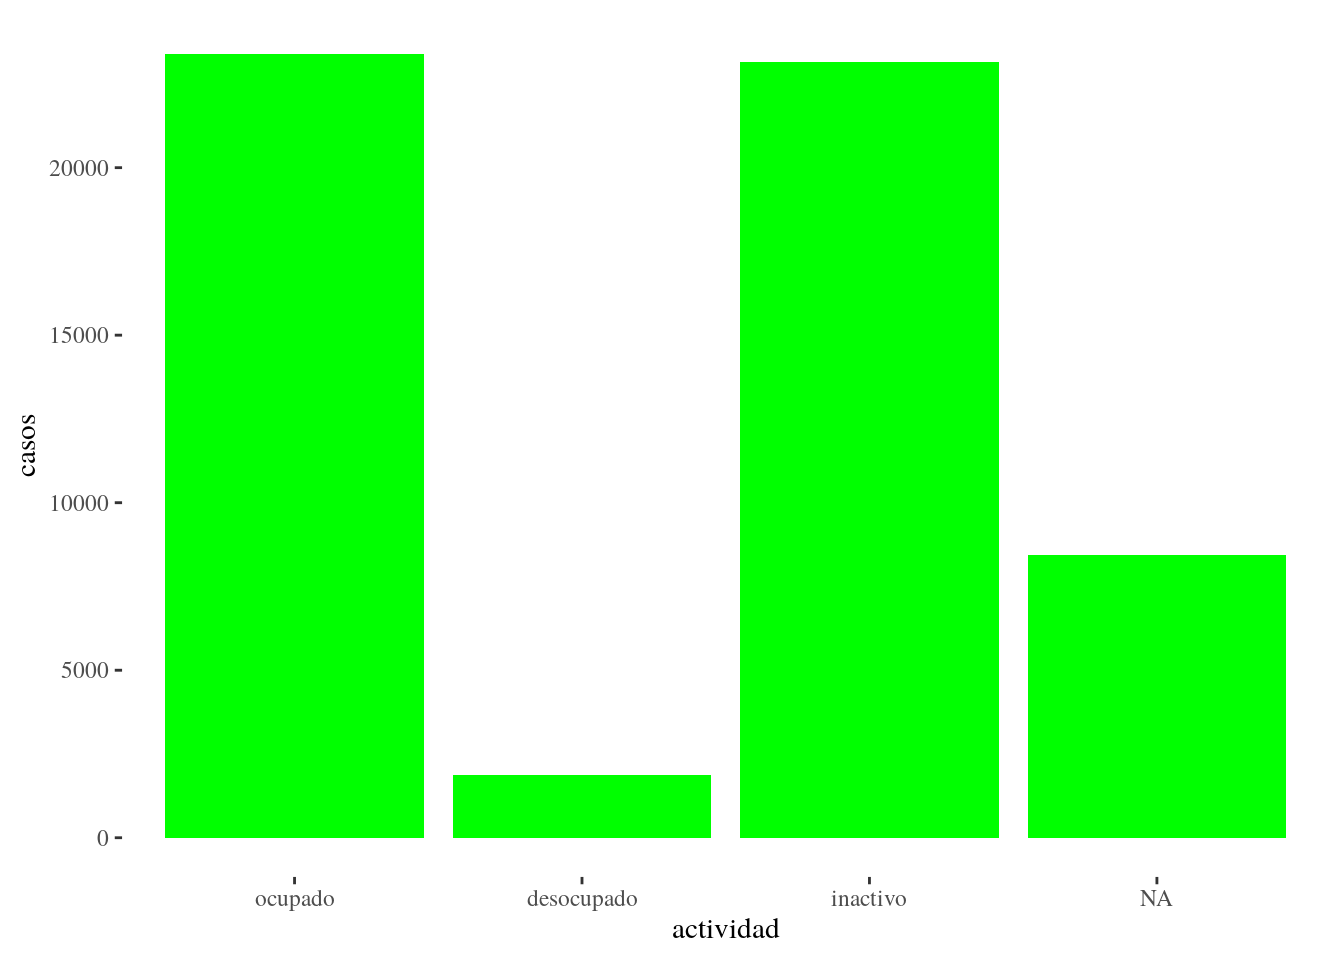
\includegraphics{EstadisticaParaCienciasSocialesConR_files/figure-latex/unnamed-chunk-31-1.pdf}
\caption{\label{fig:unnamed-chunk-31}Condición laboral: frecuencias absolutas (barras adyacentes).}
\end{figure}

La categoría NA (not available) reúne a quienes no respondieron al cuestionario y a los menores de 10 años, que no se les hace la pregunta.

\begin{figure}
\centering
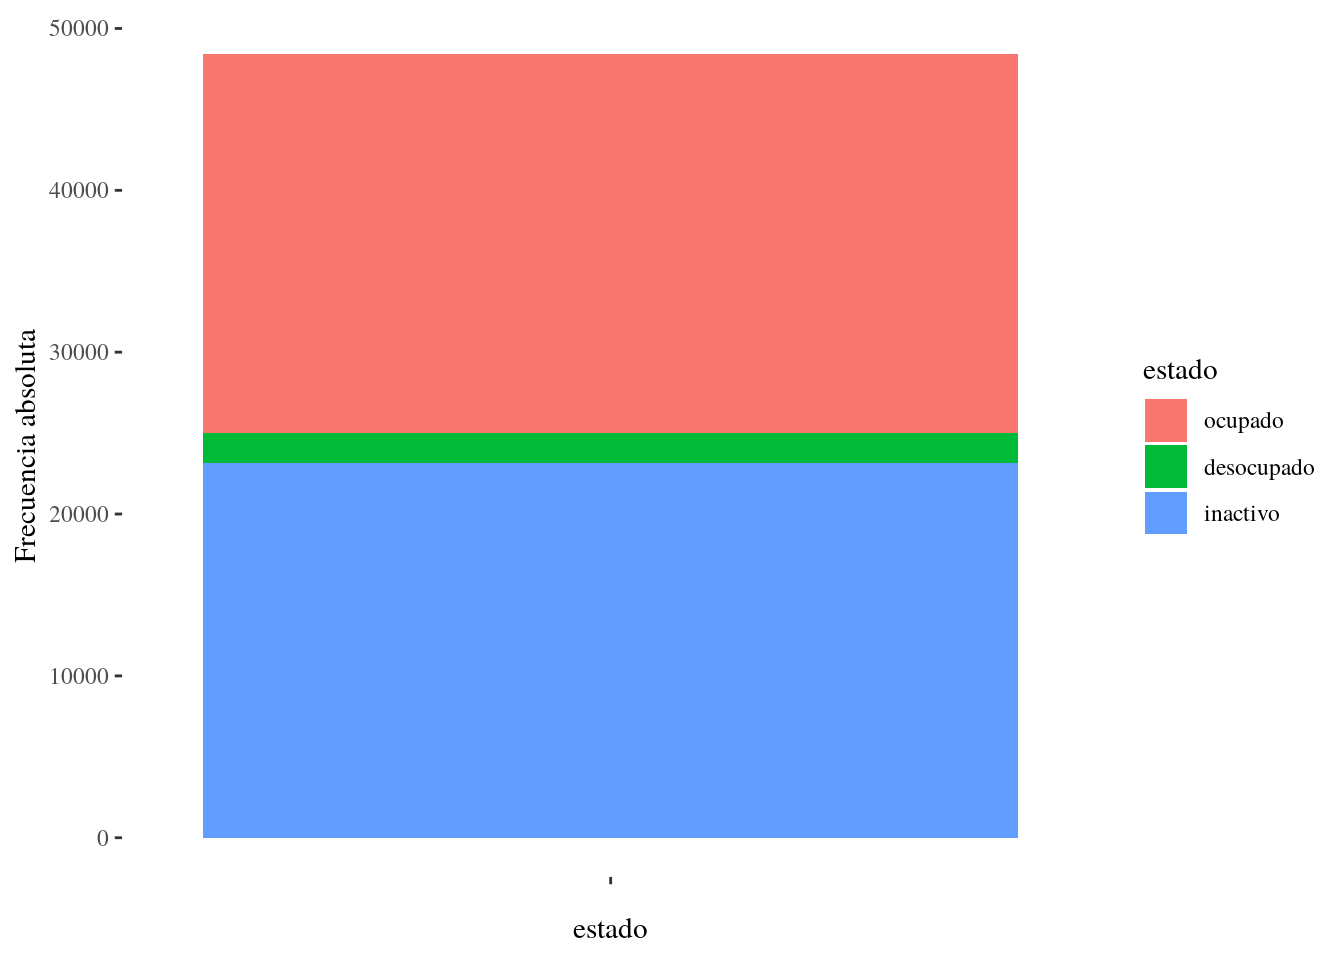
\includegraphics{EstadisticaParaCienciasSocialesConR_files/figure-latex/unnamed-chunk-32-1.pdf}
\caption{\label{fig:unnamed-chunk-32}Condición laboral: frecuencias absolutas (barras apiladas).}
\end{figure}

O bien, en relativos:

\begin{figure}
\centering
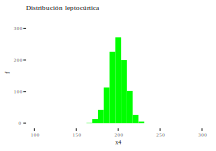
\includegraphics{EstadisticaParaCienciasSocialesConR_files/figure-latex/unnamed-chunk-33-1.pdf}
\caption{\label{fig:unnamed-chunk-33}Condición laboral: frecuencias relativas (barras apiladas).}
\end{figure}

Para variables categóricas también se usa el \emph{gráfico de sectores}

\begin{figure}
\centering
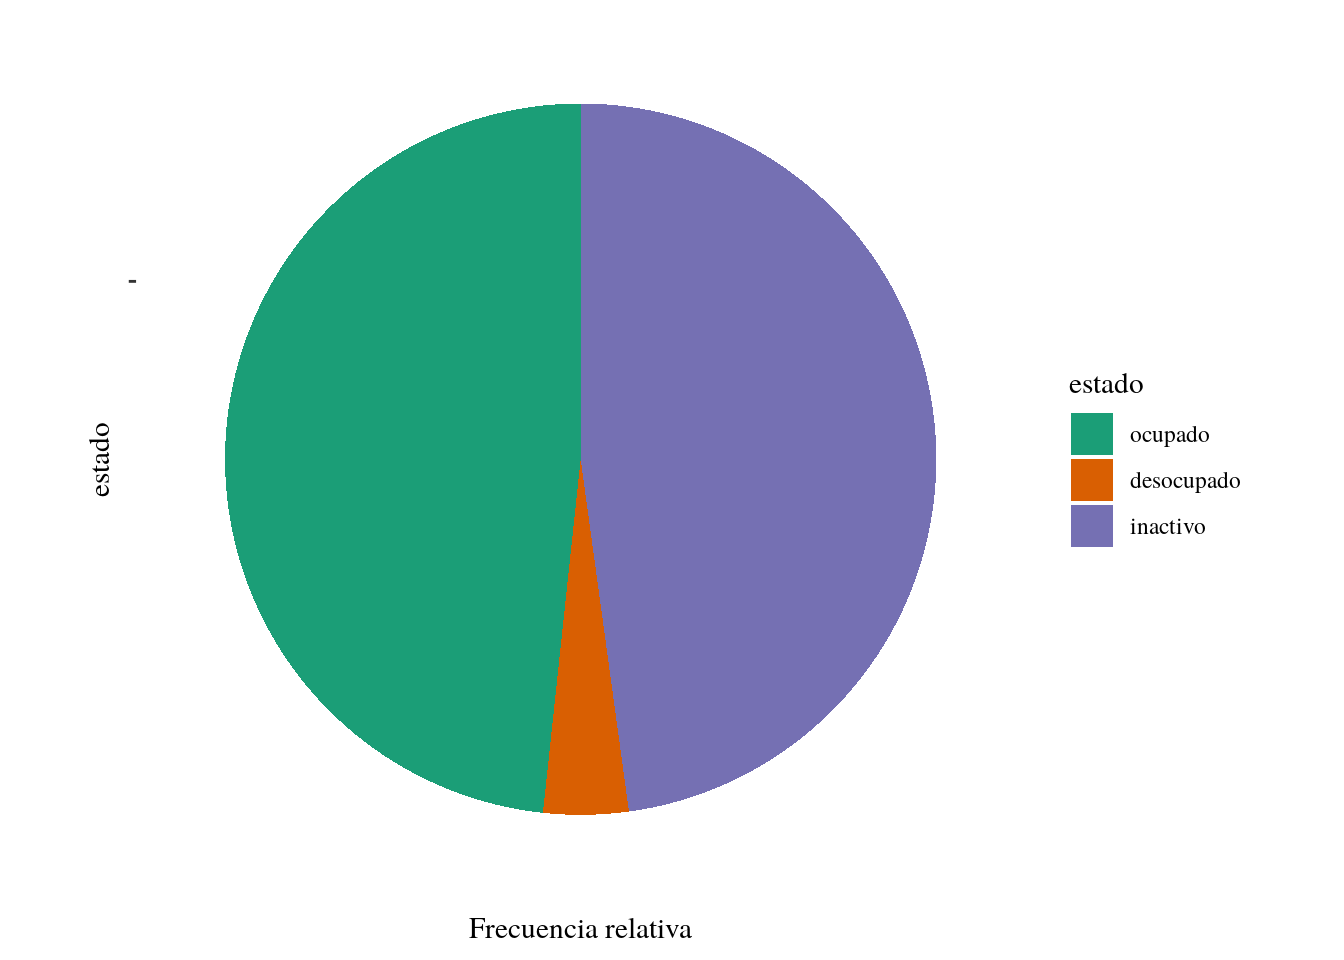
\includegraphics{EstadisticaParaCienciasSocialesConR_files/figure-latex/unnamed-chunk-34-1.pdf}
\caption{\label{fig:unnamed-chunk-34}Condición laboral: frecuencias relativas (gráfico de sectores).}
\end{figure}

Este gráfico solo es adecuado cuando la variable tiene pocas categorías (no más de cuatro) y además cuando las frecuencias difieren sustancialmente. De lo contrario, resulta muy difícil apreciar diferencias entre ángulos, éstas son mucho más claras entre alturas de barras. La opción de agregar una leyenda con los porcentajes resuelve este problema, pero hace perder parte de la claridad visual del gráfico.

La representación gráfica de la tabla de frecuencias de variables cuantitativas (categorizadas), se llama histograma:

\begin{figure}
\centering
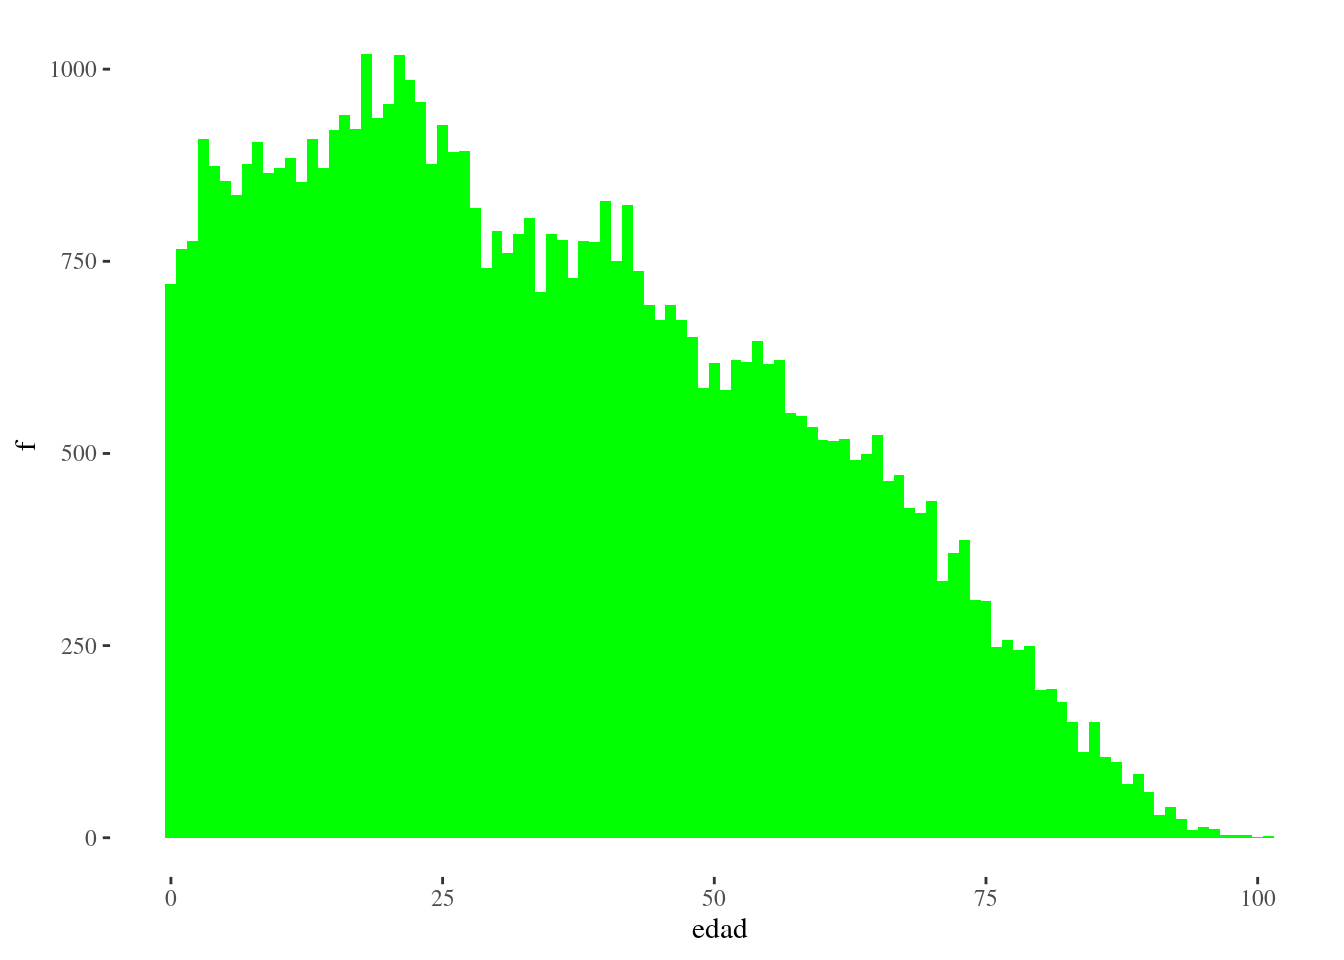
\includegraphics{EstadisticaParaCienciasSocialesConR_files/figure-latex/unnamed-chunk-35-1.pdf}
\caption{\label{fig:unnamed-chunk-35}Histograma de edades.}
\end{figure}

El ancho de los rectángulos es la amplitud de las categorías que resultan de la categorización. Esta siempre se realiza con el criterio de intervalos iguales, que puede regularse, por ejemplo, si se toman intervalos de 5 años, el histograma queda:

\begin{figure}
\centering
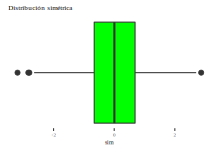
\includegraphics{EstadisticaParaCienciasSocialesConR_files/figure-latex/unnamed-chunk-36-1.pdf}
\caption{\label{fig:unnamed-chunk-36}Histograma de edades: categorías de 5 años.}
\end{figure}

Cuando estos rectángulos se unen en sus puntos medios por una poligonal, resulta el \emph{polígono de frecuencias}:

\begin{figure}
\centering
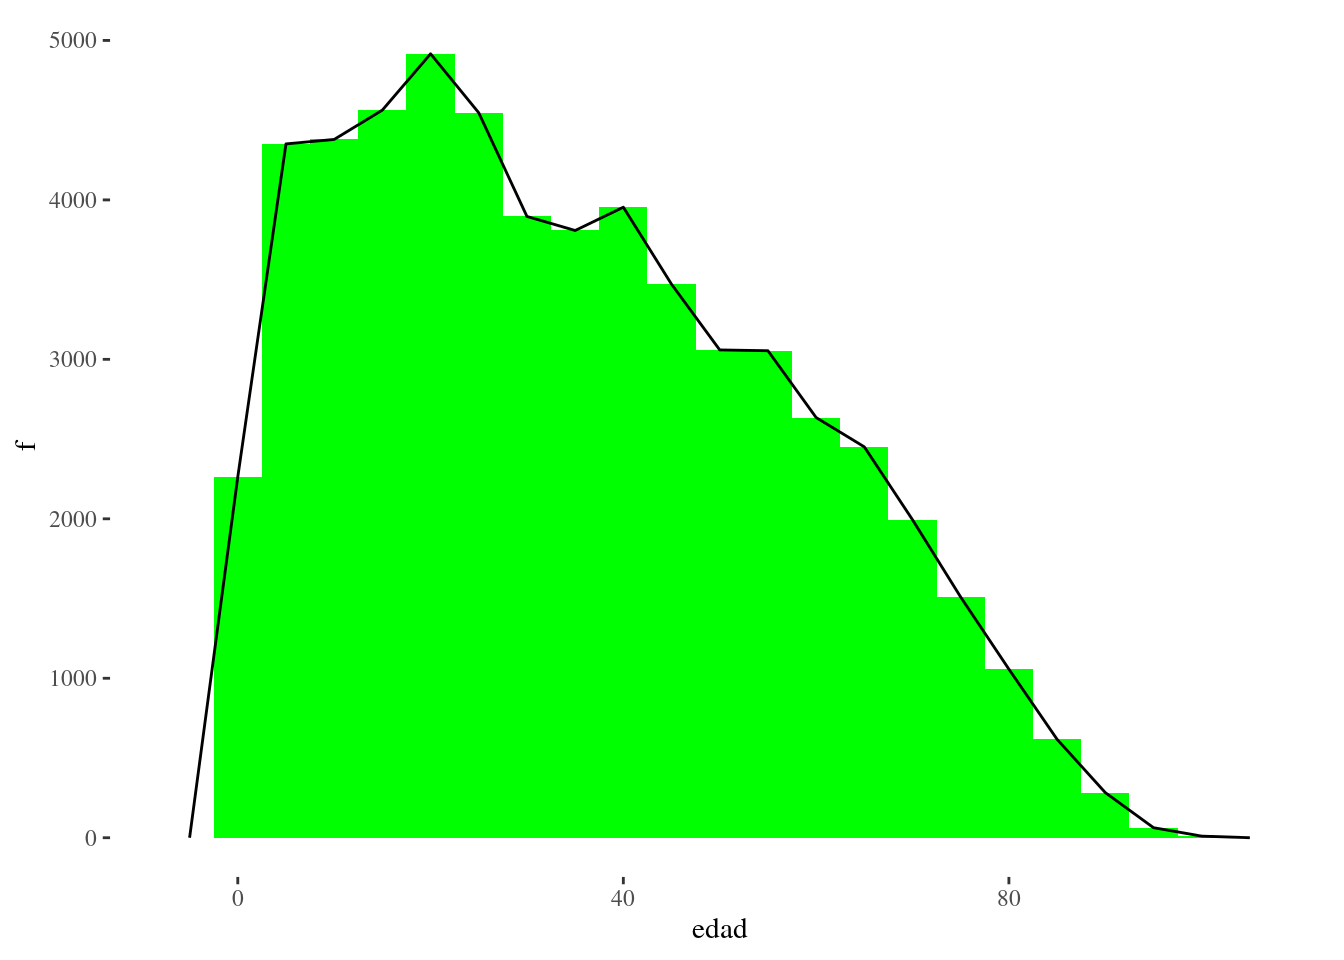
\includegraphics{EstadisticaParaCienciasSocialesConR_files/figure-latex/unnamed-chunk-37-1.pdf}
\caption{\label{fig:unnamed-chunk-37}Polígono de frecuencias de las edades sobre el histograma.}
\end{figure}

En este gráfico se agregaron dos intervalos, uno anterior al primero y uno posterior al último, cuyas frecuencias son cero, con el objetivo de ``cerrar'' el polígono sobre el eje horizontal.
El área que queda bajo este polígono es igual a la que encierran los rectángulos del histograma, y valdrá n si se grafican frecuencias absolutas ó 1 si son las relativas.

Si se muestra solo el polígono, se tiene una representacón simplificada de la distribución que sirve para apreciar aspectos que se verán más adelante: forma, dispersión, simetría, etc. Además es preferible presentar en el eje vertical, frecuencias relativas antes que absolutas.

\begin{figure}
\centering
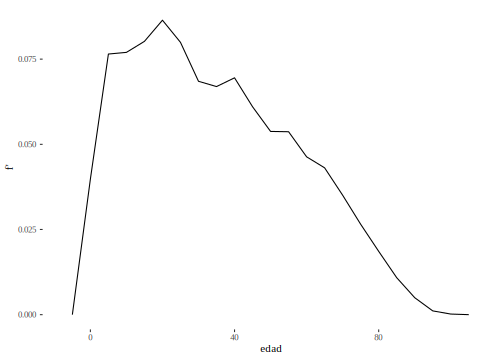
\includegraphics{EstadisticaParaCienciasSocialesConR_files/figure-latex/unnamed-chunk-38-1.pdf}
\caption{\label{fig:unnamed-chunk-38}Polígono de frecuencias de las edades.}
\end{figure}

En variables cuantitativas es posible calcular frecuencias acumuladas, por lo que también ellas pueden representarse gráficamente. Si la variable es discreta, cada valor aporta su frecuencia, que ``salta'' en el valor siguiente, por eso el gráfico tiene forma escalonada. Nuevamente, con la variable edad (CH06) de la EPH es:

\begin{figure}
\centering
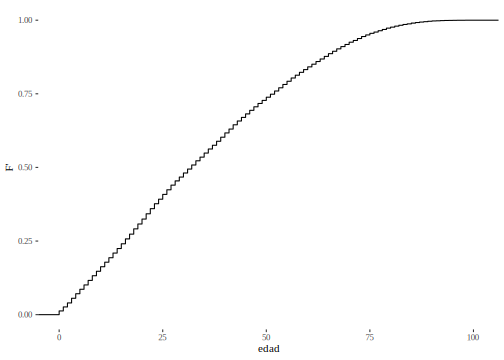
\includegraphics{EstadisticaParaCienciasSocialesConR_files/figure-latex/unnamed-chunk-39-1.pdf}
\caption{\label{fig:unnamed-chunk-39}Ojiva de las edades.}
\end{figure}

En el que el eje horizontal se indican los valores de la variable discreta edad y en el vertical las frecuencias acumuladas de cada categoría (de cada valor discreto).
Si la variable es continua, las frecuencias se van acumulando gradualmente a medida que aumenta el valor de la variable, el siguiente gráfico muestra las frecuencias acumuladas de los pesos de un conjunto grande de niños (de la base \textbf{bayley}):

\begin{figure}
\centering
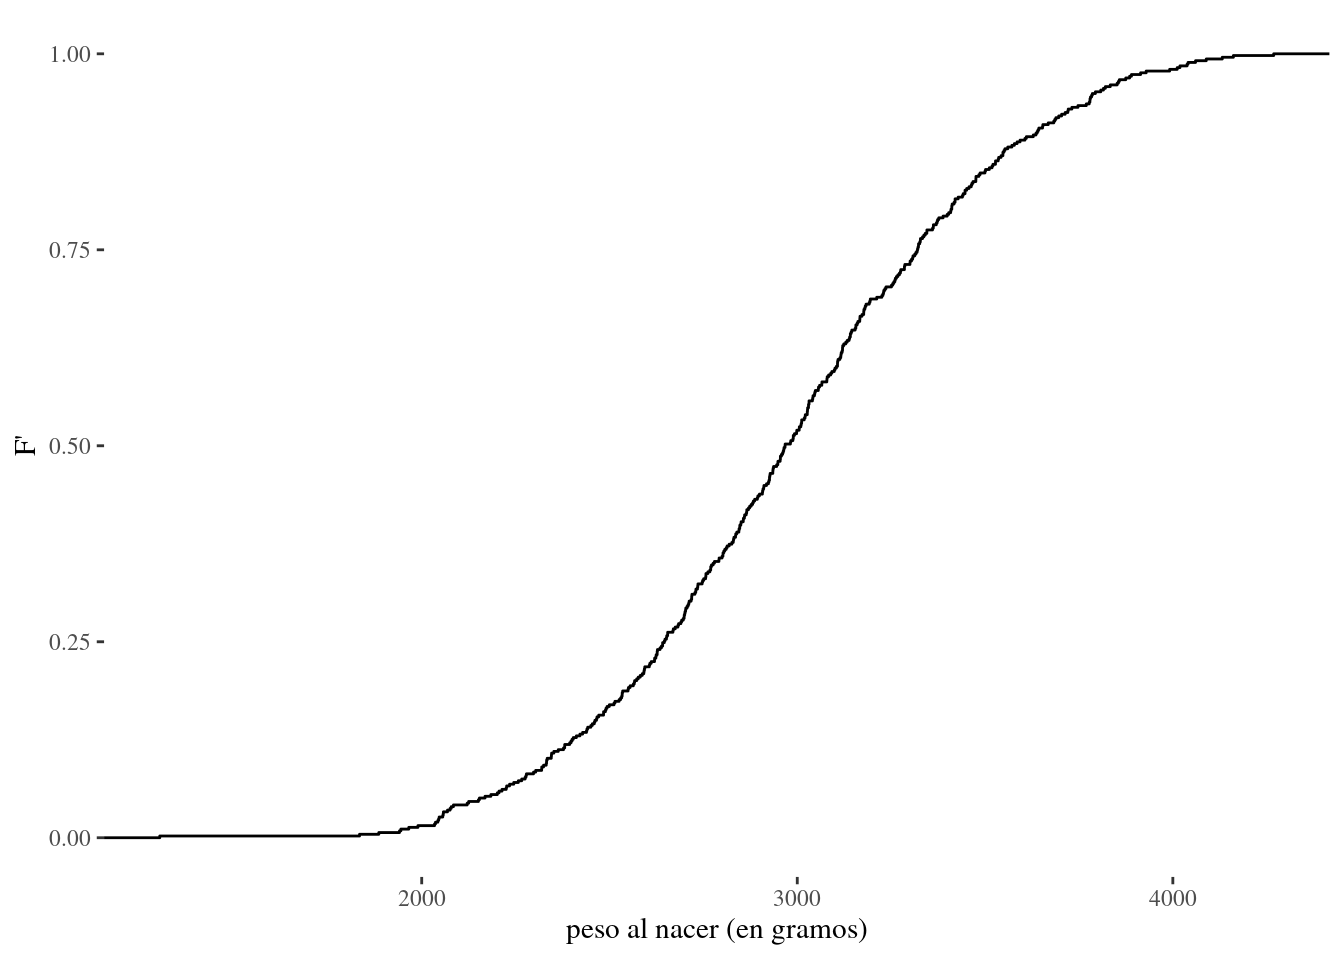
\includegraphics{EstadisticaParaCienciasSocialesConR_files/figure-latex/unnamed-chunk-40-1.pdf}
\caption{\label{fig:unnamed-chunk-40}Ojiva de los pesos al nacer.}
\end{figure}

Debido a que en la práctica las variables nunca son completamente continuas, siempre habra ``escalones'' cuyo tamaño es el de la minima medición posible de la variable (la apreciación del instrumento de medicion).

Este gráfico se llama ojiva de Galton y tiene otra virtud además de la claridad visual, ya que permite interpolar valores no observados, o que no aparecen en la tabla. Así, con el gráfico podemos responder a la pregunta ¿Qué proporción de niños tiene 2512 g o menos? La respuesta consiste en buscar el valor 2512 gramos en el eje x, e identificar la frecuencia acumulada que le corresponde.

\begin{figure}
\centering
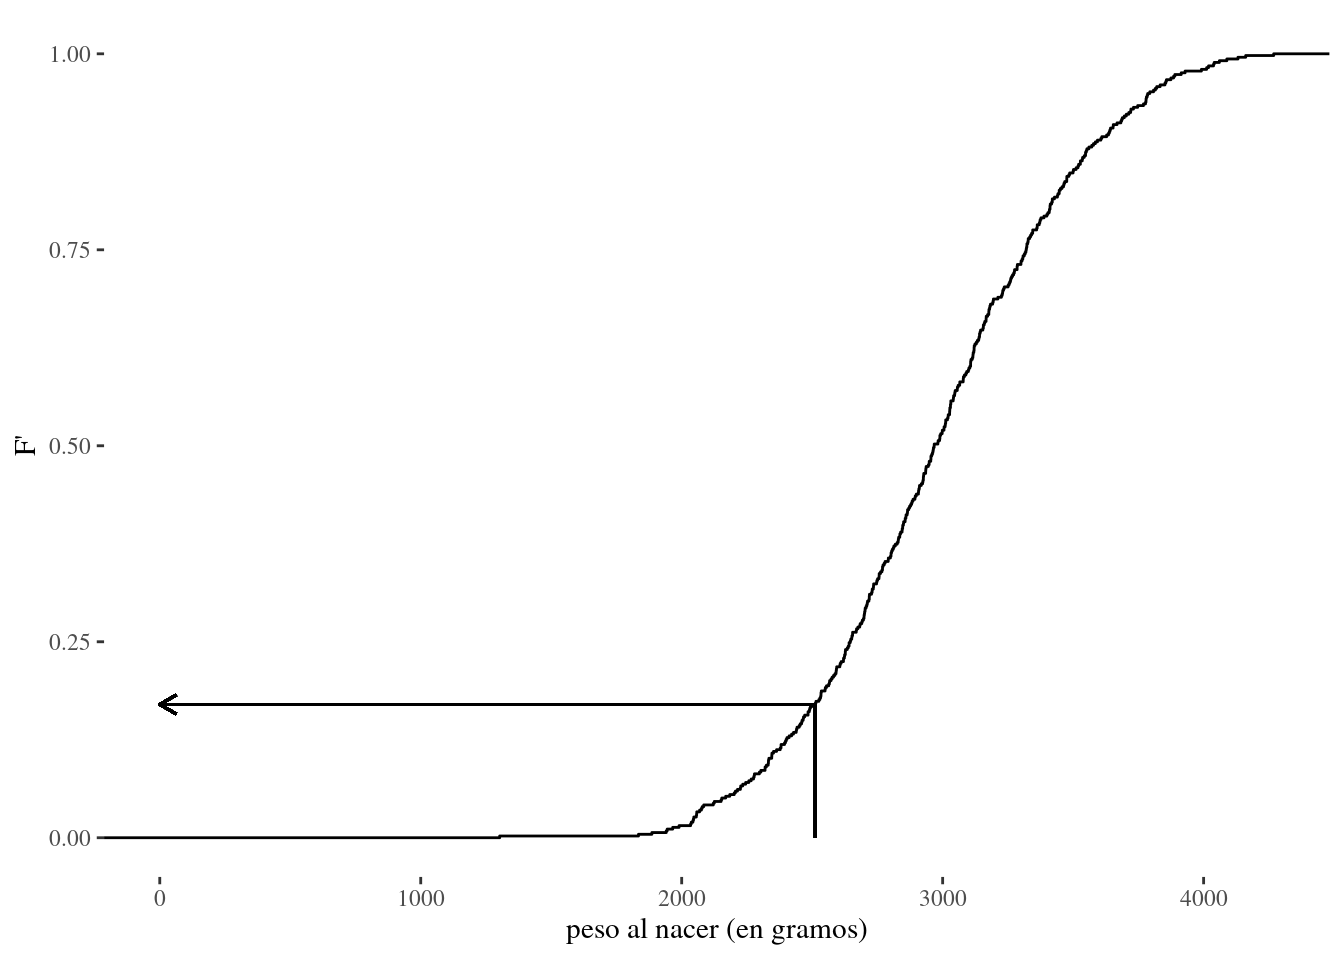
\includegraphics{EstadisticaParaCienciasSocialesConR_files/figure-latex/unnamed-chunk-41-1.pdf}
\caption{\label{fig:unnamed-chunk-41}Estimación de la frecuencia acumulada para un valor del peso al nacer.}
\end{figure}

En este ejemplo, la ordenada (valor en el eje vertical) correspondiente a los 2512 gramos es aproximadamente 0,17, este resultado se lee diciendo que, de esta muestra, el 17\% de los niños nació con 2512 gramos o menos. En los capítulos siguientes veremos otras aplicaciones útiles de este procedimiento.

Además, el establecimiento de los límites de los intervalos según el criterio proporcional, puede realizarse en base a este gráfico. Según cuántos intervalos se quiera construir, se ubican los puntos correspondientes a las frecuencias acumuladas en el eje vertical y se buscan los valores de la variable (eje horizontal), que delimitan los intervalos. Por ejemplo, para cuatro intervalos, cada uno debe contener aproximadamente el 25\% de los casos, que corresponden a las frecuencias acumuladas de 25, 50 y 75\%.

\begin{figure}
\centering
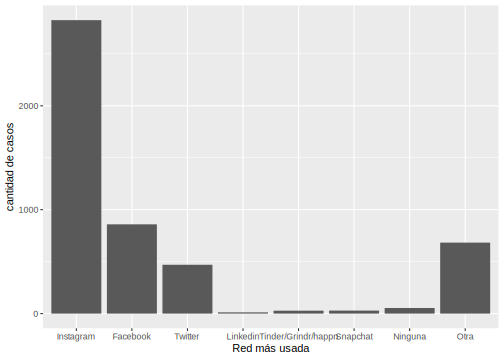
\includegraphics{EstadisticaParaCienciasSocialesConR_files/figure-latex/unnamed-chunk-42-1.pdf}
\caption{\label{fig:unnamed-chunk-42}Identificación de los valores de la variable para determinadas frecuencias absolutas.}
\end{figure}

Los valores hallados corresponden a 2646, 2968 y 3320 gramos. Que quiere decir que un cuarto de los niños nació con pesos entre el mínimo y 2646, otro cuarto pesó entre 2646 y 2968 gramos, y así con los demás. La distribución de frecuencias de esta variable así categorizada resulta:

\begin{longtable}[]{@{}lc@{}}
\caption{\label{tab:unnamed-chunk-43}Distribución de los pesos al nacer categorizados en cuatro intervalos proporcionales.}\tabularnewline
\toprule
Peso.nacCat & f\tabularnewline
\midrule
\endfirsthead
\toprule
Peso.nacCat & f\tabularnewline
\midrule
\endhead
(1302.5,2646.5{]} & 113\tabularnewline
(2646.5,2967.5{]} & 113\tabularnewline
(2967.5,3319.8{]} & 113\tabularnewline
(3319.8,4268.5{]} & 114\tabularnewline
\bottomrule
\end{longtable}

\hypertarget{la-expresion-resumida-de-la-informacion}{%
\chapter{La expresión resumida de la información}\label{la-expresion-resumida-de-la-informacion}}

La segunda etapa en la descripción de datos consiste en calcular medidas que los resuman, que los expresen de manera sintética. Esta etapa implica un nuevo alejamiento de la información bruta, ya que se pierde de vista no solo a los individuos -presentes en la matriz de datos-, sino también a las distribuciones de frecuencia. La ventaja de resumir es la posibilidad de presentar la información de modo muy sintético; con unas pocas medidas descriptivas se ofrece bastante información sobre los datos que se observan.

Estas medidas requieren operaciones de diferente nivel de complejidad, por lo que apelan a diferentes propiedades de las escalas de medición, entonces no serán las mismas las medidas que se puedan calcular en una escala nominal que en una ordinal, intervalar o proporcional.

El objetivo de describir el conjunto de datos se logrará indicando tres tipos diferentes de medidas. En primer lugar, haremos referencia a las medidas de \textbf{posición}. Estas medidas indican en torno a qué valores se distribuyen las observaciones. En segundo lugar, mencionaremos las medidas de \textbf{dispersión} (conocidas también como de \textbf{variabilidad}), que muestran si los datos están concentrados alrededor de las medidas de centralidad o si están alejados de esas medidas centrales. En tercer lugar, se describe la \textbf{forma} que toma la distribución, medida con dos indicadores: \textbf{simetría} y \textbf{curtosis}.

A los fines de la notación usada para referirse a cada una de estas
medidas descriptivas, asumiremos que trabajamos sobre datos provenientes de una muestra, de la que \emph{n} representa la cantidad de casos observados.

\hypertarget{medidas-de-posicion}{%
\section{Medidas de posición}\label{medidas-de-posicion}}

Como las operaciones que pueda hacerse entre las categorías dependen del nivel de medición de las variables, las medidas que se puedan calcular también dependerán del nivel de medición. Por eso las presentaremos separadamente para cada nivel, siempre recordando que las operaciones que son válidas a un determinado nivel de medición también son válidas para niveles más altos. Por ejemplo: lo que pueda hacerse con variables nominales, vale también para ordinales y métricas, con los ajustes de casa caso.

\hypertarget{variables-nominales-proporciones}{%
\subsection{Variables nominales: proporciones}\label{variables-nominales-proporciones}}

Cuando se trabaja con una variable de nivel nominal, una manera
sintética de presentar la información que ofrece la tabla de
distribución de frecuencias es indicando la \textbf{proporción} de casos que se encuentran en una determinada categoría. Se trata de la frecuencia relativa simple (f') de una categoría particular. La siguiente es la distribución de las respuestas a la pregunta ``¿Con cuál de las siguientes frases está Ud. más de acuerdo?'' (P8STGBS), proveniente de la base latinobarómetro:

\begin{longtable}[]{@{}lcc@{}}
\toprule
¿Con qué frase está más de acuerdo? & f & f'\tabularnewline
\midrule
\endhead
Se puede confiar en la mayoría de las personas & 0.143 & 14.3\tabularnewline
Uno nunca es lo suficientemente cuidadoso en el trato con los demás & 0.857 & 85.7\tabularnewline
Total & 1 & 100\tabularnewline
\bottomrule
\end{longtable}

Podemos indicar la proporción de personas que respondió que se puede confiar caso como 0.143, que puede también expresarse como 14.3\%. La elección de cuál categoría se elige para indicar la proporción depende de los objetivos de la descripción. Al elegir una categoría se llama la atención sobre ella, se la destaca, ya que la proporción restante incluye a todas las demás categorías, los ``otros''. Esa proporción restante se obtiene restando de 1 (uno) la proporción indicada, o restando de 100 (cien) si ha expresado como porcentaje. En este ejemplo, diremos que 0.857 (que proviene de hacer 0.857) es la proporción de quienes no creen que se pueda confiar, o bien que éstos representan el 85.7\% (85.7).

\begin{longtable}[]{@{}c@{}}
\toprule
\endhead
\begin{minipage}[t]{0.97\columnwidth}\centering
La \textbf{proporción} es la frecuencia relativa correspondiente a una categoría particular. Usualmente se expresa como porcentaje. Se indica como \(p\).\strut
\end{minipage}\tabularnewline
\bottomrule
\end{longtable}

Esta medida descriptiva se usa a menudo cuando la variable nominal tiene solo dos categorías (variable dicotómica), ya que se presenta la proporción de una de ellas e inmediatamente se sabe que el complemento es la proporción de la otra.

Esta medida ya apareció al definir la proporción como el cociente entre la frecuencia propia de la categoría y el total de casos. Esta
proporción puede también indicarse en variables de nivel de medición
superior al nominal, pero no resulta de interés cuando hay gran cantidad de categorías. Así, por ejemplo, si se trata de la distribución de las notas de un parcial, no resulta útil indicar cuál es la proporción de cada calificación e indicar algo como ``el 20\% sacó 8'' (lo que se vería en una tabla de distribución de frecuencias de las notas). Por el contrario, es común construir variables nominales a partir de las notas y, sí es de mucho interés indicar, por ejemplo, la proporción de \emph{promocionados}, o la proporción de quienes \emph{quedaron libres}, luego de haber categorizado las notas con un criterio teórico (el que define quiénes son los promocionados, regulares y libres)

\hypertarget{variables-nominales-tasas}{%
\subsection{Variables nominales: tasas}\label{variables-nominales-tasas}}

Se define habitualmente como \textbf{tasa} a la frecuencia relativa de un
fenómeno en referencia a una población total, con la característica de tener en cuenta un período de tiempo. También es común el uso del
término cuando se trata de hechos de poca incidencia, es decir que su
frecuencia es pequeña. En esos casos se la suele expresar cada 1.000,
cada 10.000, o inclusive cada 100.000 casos, en lugar de porciento. Por ejemplo, la tasa de desocupación en Argentina se define como la proporción de personas desocupadas, respecto del total de personas activas. Estas últimas son quienes tienen una ocupación o que sin tenerla la están buscando activamente. Está compuesta por la población ocupada más la población desocupada arrobaINDEC2018.

Las tasas de mortalidad por causas, indican la proporción de muertes ocurridas en un período de tiempo (usualmente un año), en un espacio geográfico (país, provincia, etc) por una determinada causa, respecto del total de la población que vivía a la mitad de ese año.

\hypertarget{variables-nominales-razones}{%
\subsection{Variables nominales: razones}\label{variables-nominales-razones}}

La palabra \textbf{razones} se usa a menudo para referirse a cocientes
calculados entre conjuntos que no tienen elementos en común. Por
ejemplo, se llama razón de masculinidad a la cantidad de hombres por
cada 100 mujeres que hay en una población. Se obtiene dividiendo el
total de varones por el total de mujeres (y luego multiplicando por
100), que son dos conjuntos que no se superponen. Esta medida se conoce también como índice de masculinidad.

Según el censo de 2010, la siguiente es el distribución por sexos de la población de Argentina en ese momento:

\begin{longtable}[]{@{}lcc@{}}
\toprule
sexo & personas & prop.sexos\tabularnewline
\midrule
\endhead
varones & 19523766 & 0.487\tabularnewline
mujeres & 20593330 & 0.513\tabularnewline
Total & 40117096 & 1.000\tabularnewline
\bottomrule
\end{longtable}

La proporción de varones es 48.7\% y la de mujeres de 51.3\%; se calculan respecto de la población total. La razón de feminidad se obtiene dividiendo el total de mujeres en el de varones y a la inversa para la de masculinidad. El cociente \(\frac{20593330}{19523766}*100\), que es 105.5 indica que hay en la población 105 mujeres por cada 100 varones.

La diferencia entre una razón y una tasa es que en la primera, el numerador no está incluido en el denominador. Las tasas a veces son llamadas \textbf{ratio}.

\hypertarget{variables-nominales-el-modo}{%
\subsection{Variables nominales: el modo}\label{variables-nominales-el-modo}}

El \textbf{modo}, o \textbf{moda}, o \textbf{valor modal} es el valor de la variable
(la categoría) que tiene la mayor frecuencia. Dicho de otra manera, el valor de la variable más frecuentemente observado. Esta medida no requiere ningún cálculo, no exige ninguna propiedad de la escala de
medición, por lo tanto se puede indicar en variables desde el nivel
nominal, es decir en todos los niveles de medición.

Por ejemplo, la variable \emph{carrera que cursa}, tiene la siguiente distribución:

\begin{longtable}[]{@{}lcc@{}}
\toprule
carrera & f & f'\tabularnewline
\midrule
\endhead
Educación & 44 & 0.29\tabularnewline
Psicología & 48 & 0.32\tabularnewline
Psicopedagogía & 58 & 0.39\tabularnewline
Total & 150 & 1.00\tabularnewline
\bottomrule
\end{longtable}

El modo es Psicopedagogía, que es la categoría de mayor frecuencia. Debe cuidarse de no cometer el error de señalar la frecuencia 58 como el modo; el modo no es la frecuencia más alta, sino la categoría de la variable que tiene mayor frecuencia. Para hallarlo, se identifica la más alta de las frecuencias y se señala la categoría que le corresponde. Puede usarse la frecuencia absoluta o la relativa para determinar cuál es el modo de la distribución.

La pregunta ``¿Con cuál de las siguientes frases está Ud. más
de acuerdo?'' (P8STGBS), procedente de la base Latinobarómetro, tiene la siguiente distribución de frecuencias:

\begin{longtable}[]{@{}lc@{}}
\toprule
P8STGBS & f\tabularnewline
\midrule
\endhead
La democracia es preferible a cualquier otra forma de gobierno & 10785\tabularnewline
En algunas circunstancias, un gobierno autoritario puede ser preferible a uno democrático & 2526\tabularnewline
A la gente como uno, nos da lo mismo un régimen democrático que uno no democrático & 5075\tabularnewline
\bottomrule
\end{longtable}

Allí, la categoría modal es la que privilegia a la democracia como sistema de gobierno.

Si se trata de una variable de mayor nivel de medición, no hay ninguna diferencia. La variable \emph{concepto que los docentes asignan a los alumnos} tiene la distribución de frecuencias siguiente:

\begin{longtable}[]{@{}lc@{}}
\toprule
concepto & f\tabularnewline
\midrule
\endhead
Excelente & 150\tabularnewline
Muy bueno & 350\tabularnewline
Bueno & 200\tabularnewline
Satisfactorio & 120\tabularnewline
No satisfactorio & 50\tabularnewline
Total & 870\tabularnewline
\bottomrule
\end{longtable}

En este ejemplo, 350 es la frecuencia más alta, por lo tanto, la
categoría que a ella corresponde es el modo: el modo de la distribución es ``Muy bueno''.

\begin{longtable}[]{@{}c@{}}
\toprule
\endhead
\begin{minipage}[t]{0.97\columnwidth}\centering
El \textbf{modo} es la categoría -o el valor- de la variable que tiene mayor frecuencia. Se indica \(M_o\).\strut
\end{minipage}\tabularnewline
\bottomrule
\end{longtable}

Cuando se trabaja sobre variables intervalares o proporcionales
discretas no hay diferencia en la identificación del modo de la
distribución. El \emph{número de materias que tienen aprobadas alumnos que han terminado de cursar el primer año} de su carrera se distribuye así:

\begin{longtable}[]{@{}lc@{}}
\toprule
Cantidad de materias aprobadas & f\tabularnewline
\midrule
\endhead
0 & 30\tabularnewline
1 & 150\tabularnewline
2 & 200\tabularnewline
3 & 300\tabularnewline
4 & 250\tabularnewline
5 & 200\tabularnewline
6 & 20\tabularnewline
Total & 1150\tabularnewline
\bottomrule
\end{longtable}

En esta distribución, el modo es 3 materias aprobadas (\(M_o = 3\)), que es la categoría que tiene mayor frecuencia. Expresamos esto como ``la mayor cantidad de alumnos que terminaron de cursar primer año han aprobado tres materias''.

Puede suceder que en una distribución no haya una única categoría de
mayor frecuencia, sino que dos o más compartan la mayor frecuencia. Para 160 alumnos clasificados según la facultad en que cursan su carrera, tenemos:

\begin{longtable}[]{@{}lc@{}}
\toprule
Facultad a la que pertenece & f\tabularnewline
\midrule
\endhead
Arquitectura & 50\tabularnewline
Ingeniería & 40\tabularnewline
Psicología & 50\tabularnewline
Sociales & 20\tabularnewline
Total & 160\tabularnewline
\bottomrule
\end{longtable}

Vemos aquí que hay dos categorías que presentan la mayor frecuencia:
Arquitectura y Psicología. Decimos en este caso que la distribución es \textbf{bimodal} que quiere decir que tiene dos modos.

\begin{longtable}[]{@{}c@{}}
\toprule
\endhead
\begin{minipage}[t]{0.97\columnwidth}\centering
Una distribución es \textbf{bimodal} cuando dos categorías tienen la mayor frecuencia. Si son más las categorías que comparten la mayor frecuencia, la distribución se denomina \textbf{multimodal}.\strut
\end{minipage}\tabularnewline
\bottomrule
\end{longtable}

Una representación gráfica de una distribución bimodal, para la variable \emph{número de respuestas correctas en una prueba de opción múltiple}, la siguiente:

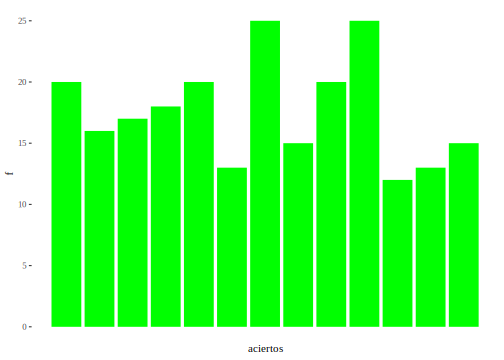
\includegraphics{EstadisticaParaCienciasSocialesConR_files/figure-latex/unnamed-chunk-51-1.pdf}

Como modo en 6 y 9 aciertos, por eso se llama bimodal.

La moda tiene el inconveniente de ser independiente de la mayor parte de los datos, por lo que es sensible a cambios en los valores de la
distribución. En efecto, las siguientes dos muestras de 130 escuelas
tienen la misma moda (\(M_o = Pública\)), aunque son muy dispares:

\begin{longtable}[]{@{}lclc@{}}
\toprule
Gestión de la escuela & f & Gestión de la escuela & f\tabularnewline
\midrule
\endhead
Pública & 50 & Pública & 100\tabularnewline
Privada laica & 45 & Privada laica & 20\tabularnewline
Privada confesional & 35 & Privada confesional & 10\tabularnewline
Total & 130 & Total & 130\tabularnewline
\bottomrule
\end{longtable}

\hypertarget{variables-ordinales-percentiles}{%
\subsection{Variables ordinales: percentiles}\label{variables-ordinales-percentiles}}

Como ya hemos visto, cuando las categorías de la variable están
ordenadas pueden hacerse juicios como ``mayor que'' (\(>\)) o ``menor que''
(\(<\)), y el nivel de medición es ordinal. En este tipo de variables
puede calcularse un conjunto de medidas de posición, que usan esa propiedad: la del orden entre categorías. Se trata de los \textbf{percentiles}, que se podrán también calcular para escalas superiores (intervalar y proporcional) pero no para escalas nominales, en las que el orden entre categorías no está presente.
Los percentiles usan las frecuencias relativas acumuladas, por eso solo existen para variables de nivel superior al nominal. Veamos la presentación por medio de un ejemplo, con la tabla siguiente que tiene calculadas las frecuencias acumuladas y se muestran solo ellas:

\begin{longtable}[]{@{}cc@{}}
\toprule
edad & F'\tabularnewline
\midrule
\endhead
17 & 0.00\tabularnewline
18 & 0.07\tabularnewline
19 & 0.16\tabularnewline
20 & 0.26\tabularnewline
21 & 0.36\tabularnewline
22 & 0.46\tabularnewline
23 & 0.55\tabularnewline
24 & 0.61\tabularnewline
25 & 0.68\tabularnewline
26 & 0.73\tabularnewline
27 & 0.77\tabularnewline
28 & 0.80\tabularnewline
29 & 0.83\tabularnewline
30 & 0.85\tabularnewline
31 & 0.87\tabularnewline
32 & 0.89\tabularnewline
33 & 0.91\tabularnewline
34 & 0.92\tabularnewline
35 & 0.93\tabularnewline
36 & 0.94\tabularnewline
37 & 0.95\tabularnewline
38 & 0.95\tabularnewline
39 & 0.96\tabularnewline
40 & 0.96\tabularnewline
41 & 0.97\tabularnewline
42 & 0.97\tabularnewline
43 & 0.98\tabularnewline
44 & 0.98\tabularnewline
45 & 0.98\tabularnewline
46 & 0.99\tabularnewline
47 & 0.99\tabularnewline
48 & 0.99\tabularnewline
49 & 0.99\tabularnewline
50 & 0.99\tabularnewline
51 & 1.00\tabularnewline
52 & 1.00\tabularnewline
53 & 1.00\tabularnewline
54 & 1.00\tabularnewline
\bottomrule
\end{longtable}

La frecuencia acumulada 0.26 indica que el 26\% de los estudiantes tiene 20 años o menos. Se dice que el valor 20 años es el percentil 26 y se indica \(P_{26}\). El ``percentil'' en sí mismo no es una medida descriptiva, para que lo sea se debe especificar \emph{qué} percentil es el que se calcula. En este ejemplo, cada frecuencia acumulada conduce a un percentil particular. El percentil 68 de la variable es 25 años, y se escribe \(P_{68} = 25\) años. Estas medidas se definen como el valor de la variable que deja por debajo un determinado porcentaje de observaciones.

Los percentiles tienen utilidad como medidas resumen cuando hay un volumen importante de observaciones, de lo contrario, es preferible mostrar la serie de datos. Su aplicación es que permiten describir cada valor de la variable de manera relativa al conjunto completo. Si la nota de un individuo corresponde al percentil 95, se sabe que es una nota alta, porque el 95\% de todos los sujetos tiene una nota com esa o inferior. Eso puede expresarse diferente como: solo el 5\% del conjunto tiene nota superior a la de él.

A continuación veremos algunos medidas que se definen del mismo modo que los percentiles; en base a las frecuencias relativas acumuladas.

\hypertarget{variables-ordinales-la-mediana}{%
\subsection{Variables ordinales: la mediana}\label{variables-ordinales-la-mediana}}

La \textbf{mediana} es el percentil 50, es decir que se define como el valor de la variable que deja por debajo la mitad del total de observaciones. Es importante tener en cuenta que se trata de la mitad de los casos y no la mitad de las categorías. La siguiente distribución presenta en serie simple ordenada el número de sesiones de psicoterapia que recibieron 9 pacientes internados en un hospital:

\[2, 2, 3, 5, 7, 10, 15, 19, 50\]

La mediana de estos datos es 7, porque es el valor que deja cuatro casos por debajo y también cuatro casos por encima. Atención a que la serie simple debe estar ordenada para poder identificar a la mediana.

Si la cantidad de observaciones fuera par como por ejemplo:

\[2, 2, 3, 5, 7, 10, 15, 19\]

El punto de corte correspondiente a la mitad de las observaciones se
ubica entre 5 y 7, en este caso, la mediana es el promedio entre los dos valores centrales, que es 6.

Cuando hay valores repetidos en la parte central no resulta posible
indicar la mediana, por ejemplo si la serie fuera:

\[2, 3, 7, 7, 7, 10, 15, 19\]

No puede señalarse a 7 como la mediana, porque es superado por tres
valores (10, 15 y 19) pero supera solo a dos (2 y 3).

La mediana es una medida muy adecuada cuando se necesitan resumir datos que provienen de escalas ordinales o de nivel superior. Sin embargo, su cálculo no aporta nada en series simples con pocos casos (como los que acabamos de ver) ya que allí es más sencillo mostrar el conjunto completo de datos y no usar medidas resumen. Los ejemplos sirven para ilustrar el concepto, pero no se usa en la práctica. Las operaciones de resumen se justifican cuando se tiene un conjunto grande de datos.

\begin{longtable}[]{@{}c@{}}
\toprule
\endhead
\begin{minipage}[t]{0.97\columnwidth}\centering
Se denomina \textbf{mediana} al valor de la variable que deja por debajo a la mitad de las observaciones. La mediana deja la misma cantidad de casos por debajo y por encima de ella. Se indica \(M_{dn}\).\strut
\end{minipage}\tabularnewline
\bottomrule
\end{longtable}

Veamos la forma de reconocer a la mediana cuando los datos están
presentados en una distribución de frecuencias. La siguiente es una
clasificación de hogares por nivel socioeconómico:

\begin{longtable}[]{@{}lcc@{}}
\toprule
Nivel socioeconómico & f (número de hogares) & F\tabularnewline
\midrule
\endhead
Marginal & 40 & 40\tabularnewline
Bajo & 100 & 140\tabularnewline
Medio-bajo & 120 & 260\tabularnewline
Medio & 150 & 410\tabularnewline
Alto & 30 & 440\tabularnewline
Total & 440 &\tabularnewline
\bottomrule
\end{longtable}

El valor de la variable que acumula el 50\% de los casos, es el que ocupa el lugar 220, que es mitad de los 440 casos del total. La serie ordenada de esta distribución, coloca a los 40 hogares marginales en lso primeros 40 lugares, pero indistintamente, porque no hay orden entre los hogares al interior de la categoría. Según la tabla, hasta la categoría ``medio-bajo'' se acumulan 260 hogares y hasta la categoría anterior hay 140 acumulados. De manera que el hogar que ocupa el lugar 220 (de la serie ordenada) es uno de los que se encuentran en la categoría ``medio-bajo''. Diremos así que la mediana de esta distribución es ``medio-bajo''. Como puede verse, esta categoría no acumula exactamente la mitad de las observaciones, pero es la que contiene a la observación que supera a la mitad y es superada por la otra mitad. Por esa razón la leemos como la mediana, diciendo que la mitad de los hogares tiene un nivel socioeconómico medio-bajo o inferior a ese. Decir que el que acumula 220 casos es ``uno de los hogares de la categoría medio-bajo'' es impreciso, porque todos los hogares son equivalentes en su nivel socioeconómico al interior de la categoría.

Esta imprecisión también aparece si se trata de
una variable cuantitativa discreta. Si la variable es el \emph{número de síntomas} a partir de los cuales fueron diagnosticados de esquizofrenia un conjunto de pacientes:

\begin{longtable}[]{@{}lcc@{}}
\toprule
Cantidad de síntomas & f (número de pacientes) & F\tabularnewline
\midrule
\endhead
2 & 30 & 30\tabularnewline
3 & 60 & 90\tabularnewline
4 & 70 & 160\tabularnewline
5 & 90 & 250\tabularnewline
Total & 250 &\tabularnewline
\bottomrule
\end{longtable}

La mitad del número total de casos es de 125 (\(250/2\) ó \((1/2)*250\)), ¿cuál
es el caso que ocupa ese lugar? Vemos que hasta 3 síntomas se acumulan
90 pacientes y 160 hasta los 4. El paciente que ocupa el puesto 125 en
la serie simple ordenada es uno de los que fueron diagnosticados a
partir de 4 síntomas. Por esa razón indicamos a la mediana con ese
valor: 4, \(M_{dn} = 4\). Nuevamente encontramos que no es exactamente el
valor que acumula la mitad, sino uno de los que están en la categoría
dentro de la cual se acumula la mitad de los casos. La primera categoría
que tenga una frecuencia acumulada superior al 50\% será la que contenga
a la mediana. Es así porque la clase anterior no alcanza a acumular la
mitad de las observaciones. La lectura del resultado es que la mitad de
los pacientes fue diagnosticada de esquizofrenia en presencia de cuatro
síntomas o menos.

Sea la variable \emph{número de materias aprobadas}:

\begin{longtable}[]{@{}lcc@{}}
\toprule
Número de materias aprobadas & f & F\tabularnewline
\midrule
\endhead
0 & 30 & 30\tabularnewline
1 & 150 & 180\tabularnewline
2 & 200 & 380\tabularnewline
3 & 300 & 680\tabularnewline
4 & 250 & 930\tabularnewline
5 & 200 & 1130\tabularnewline
6 & 20 & 1150\tabularnewline
Total & 1150 &\tabularnewline
\bottomrule
\end{longtable}

La mitad de 1150 es 575, la primera frecuencia acumulada que supera a
575 es 680, que corresponde al valor 3. La mediana de esta distribución es entonces tres materias aprobadas y diremos que el 50\% de los alumnos aprobó tres materias o menos.

Cuando se trata de variables de nivel intervalar o proporcional y con
categorías agrupadas, el cálculo anterior puede refinarse. Así, primero se identifica la categoría (el intervalo) en que se encuentra la mediana, igual que en los dos ejemplos anteriores y luego se interpola dentro del intervalo para encontrar su valor exacto.

\begin{longtable}[]{@{}lcc@{}}
\toprule
Tiempo de reacción (en segundos) & f & F\tabularnewline
\midrule
\endhead
1.0 - 1.5 & 5 & 5\tabularnewline
1.5 - 2.0 & 7 & 12\tabularnewline
2.0 - 2.5 & 6 & 18\tabularnewline
2.5 - 3.0 & 3 & 21\tabularnewline
3.0 - 3.5 & 8 & 29\tabularnewline
3.5 - 4.0 & 5 & 34\tabularnewline
Total & 34 &\tabularnewline
\bottomrule
\end{longtable}

La mitad de las 34 observaciones es 17, por lo que debe encontrarse una
observación que tenga frecuencia acumulada de 17. Ese valor no aparece
en la F, el primero que lo supera es 18, entonces la mediana estará en
el intervalo 2,0-2,5. Esto es así porque hasta 2,0 se acumulan 12 casos
(la F de la categoría anterior) y hasta 2,5 se acumulan 18. Nuestros 17
casos se acumulan para un valor de la variable que está entre 2,0 y 2,5.

Debemos ahora encontrar qué valor exactamente es la mediana, dentro del
intervalo 2,0-2,5. La fórmula para este procedimiento es la siguiente:

\[M_{dn} = l_{i} + i*\left( \frac{\frac{n}{2} - F_d}{f_{p}} \right)\]

En la que:

\begin{itemize}
\item
  \(l_i\) indica el límite inferior del intervalo en que se encuentra la mediana, en este caso es 80.
\item
  \(i\) es la amplitud del intervalo, es decir la diferencia entre los límites \(2.0-2.5 = 0.5\).
\item
  \(\frac{n}{2}\) es la mitad del número total de observaciones, es este caso, 17.
\item
  \(F_d\) es la frecuencia acumulada por \textbf{d}ebajo de la categoría que contiene la mediana, en esta tabla es 12.
\item
  \(f_p\) es la frecuencia \textbf{p}ropia del intervalo en que se encuentra la mediana. Es la frecuencia absoluta (no la acumulada), en este ejemplo es 6.
\end{itemize}

Reemplazando resulta:

\[M_{dn} = 2.0 + 0.5*\left( \frac{17 - 12}{6} \right) = 2.0 + 0.5*\left( \frac{5}{6} \right) = 2.42\]

Conviene detenerse en el orden en que se realizaron las operaciones. El
signo más (+) separa términos, por lo que debe primero resolverse el
segundo de ellos y luego recién sumar 2.0. Un error frecuente es el de
sumar \(2.0 + 0.5\) y luego multiplicar por el resultado del paréntesis, eso
es incorrecto.

Por cierto que debe verificarse que el valor encontrado se ubique dentro
del intervalo; en este ejemplo, la mediana no podría ser menor que 2.0
ni mayor que 2.5. Observemos también que el número de categorías de la
variable, que es de 6, no participa en el cálculo de la mediana, de
ningún modo se trata de una categoría que esté ``al medio''.

El resultado obtenido nos dice, según la definición de la mediana que
``el 50\% de los sujetos experimentales reaccionó en un tiempo de 2.42
segundos o inferior''. Es muy importante la última parte de la lectura,
porque cuando decimos ``o inferior'' incluimos los valores por debajo del indicado. De lo contrario, si se omite ``o menos'' se estaría diciendo que la mitad de los sujetos tardó \emph{exactamente} 2.42 segundos.

La mediana encontrada, de 2.42, es un valor razonable a partir de la
observación de la tabla: la categoría de la mediana acumulaba 18 casos,
que es apenas más que la mitad de las observaciones (17), por lo que era
de esperar que la mediana apareciera cerca del límite superior del
intervalo, que es lo que sucedió.

Este procedimiento para calcular la mediana es imperfecto, porque supone que los valores están distribuidos de manera uniforme dentro de cada intervalo. Si los 6 valores que contiene el intervalo 2.0 -- 2.5, fueran
todos iguales a 2.01, por ejemplo, la mediana sería un número bastante
menor al que se calculó con este método. El uso de la interpolación solo
se justifica en situaciones en que la única información disponible es la
tabla con los valores agrupados; por el contrario, si se cuenta con la
matriz de datos, el cálculo debe hacerse usando todos los valores
observados de la variable. Como esto es largo para hacer manualmente, se
solicita a un software especializado.

\emph{Variables métricas: la media o promedio}

Si se ha alcanzado un nivel de medición intervalar o proporcional, es
posible hacer uso de las propiedades que estas escalas tienen.
Recordemos que además de designar y ordenar, las escalas intervalares
conservan las distancias entre observaciones, y las proporcionales
agregan la proporcionalidad de los valores absolutos y el carácter
absoluto del cero. En este nivel los números que representan las
categorías (o valores) pueden tratarse como tales y se puede operar con ellos. Antes de dar una definición de la media o promedio, veamos la idea intuitiva que tenemos, ya que se trata de una medida de mucho uso.
Cuando queremos calcular un promedio ``sumamos y dividimos por la
cantidad de casos''. Así, si tres personas cometen 5, 8 y 12 errores cada uno, el promedio de esa variable (número de errores) es
\(\frac{5 + 8 + 12}{3} = \frac{25}{3} = 8.33\). Usaremos la expresión
\(\overline{x}\) para referirnos a la media, con lo que el resultado se
escribe: \(\overline{x} = 8.33\) errores.

¿Cómo extenderemos esta forma de cálculo al caso en que la variable no
está presentada en serie simple sino en distribución de frecuencias?
Recordando que la frecuencia indica la cantidad de veces que cada valor
se repite, por lo que habrá que considerar cada valor tantas veces como
lo indique su frecuencia absoluta simple. Veamos un ejemplo en el que se
cuenta el número de materias aprobadas:

\begin{longtable}[]{@{}lc@{}}
\toprule
Número de materias aprobadas & f\tabularnewline
\midrule
\endhead
0 & 30\tabularnewline
1 & 150\tabularnewline
2 & 200\tabularnewline
3 & 300\tabularnewline
4 & 250\tabularnewline
5 & 200\tabularnewline
6 & 20\tabularnewline
Total & 1150\tabularnewline
\bottomrule
\end{longtable}

El valor 0 (cero) está repetido 30 veces, lo que indica que hay 30
alumnos que no han aprobado aún ninguna materia. Del mismo modo, 150
alumnos aprobaron 1 materia, etc., por lo que si estuvieran presentados
en serie simple, se sumarían los 1150 valores (30 veces el 0, 150 veces
el 1, etc.) y esa suma se dividiría por 1150. Para hacerlo sobre la
distribución de frecuencia, se multiplica cada valor de la variable por
su frecuencia (que es equivalente a sumarlo tantas veces como aparece) y
se divide por el total de casos. Resulta:

\[\overline{x} = \frac{0*30 + 1*150 + 2*200 + 3*300 + 4*250 + 5*200 + 6*20}{1150} = 3.10\]

La expresión formal de este cálculo es:

\[\overline{x} = \frac{\sum_{i = 1}^{k}{x_{i}*f_{i}}}{n}\]

En la que \(x_i\) es cada valor de la variable, \(f_i\) es su frecuencia
absoluta simple, \(k\) es el número de categorías y \(n\) es el total de
observaciones. La fórmula indica que cada valor de la variable (\(x_i\))
se multiplica por su frecuencia (\(f_i\)), se suman desde el primero
(\(i=1\)) hasta el último (\(k\)) y el resultado se divide por el total de
casos (\(n\)).

Veamos que no se trató como podríamos haber pensado rápidamente, de
sumar desde el cero hasta el seis y dividir por siete. Haber hecho eso
habría implicado dos errores: el primero es el de no considerar cuántas
veces está repetido cada valor (su frecuencia absoluta simple), el
segundo es el de confundir el número de casos (1150) con el número de
categorías (7). Este último error puede provenir de una confusión entre
la presentación en serie simple o en distribución de frecuencias. Cuando
se observa una serie simple, los valores ``sueltos'' de la variable
coinciden con sus categorías, pero cuando se agrupa, cada categoría
incluye cierta cantidad de casos que tienen el mismo valor, lo cual está
indicado en la frecuencia de cada categoría.

En el ejemplo anterior entonces, el número promedio de materias
aprobadas es 3.10. Este número no es entero y no es un valor que se
pueda observar; nadie tiene 3.10 materias aprobadas. Sin embargo, es
valioso para caracterizar a la distribución completa y para hacer
comparaciones. Por ejemplo, si en un grupo de alumnos la media es de
3,10 materias aprobadas y en otro de 3.90; puede decirse que en el
segundo grupo los alumnos han aprobado -en promedio-, más materias;
aunque ninguno haya aprobado 3.10 ni 3.90 materias.

Por el momento ofreceremos una definición operacional de la media, más
adelante podrá darse una definición conceptual, basada en sus
propiedades.

\begin{longtable}[]{@{}c@{}}
\toprule
\endhead
\begin{minipage}[t]{0.97\columnwidth}\centering
La \textbf{media} (o promedio) es un valor de la variable obtenido sumando todas las observaciones multiplicadas por su frecuencia absoluta y dividiendo el resultado en el número total de casos. Se indica como \(\overline{x}\) (equis media).\strut
\end{minipage}\tabularnewline
\bottomrule
\end{longtable}

Cuando la distribución de frecuencias presenta los datos agrupados,
aparece el problema de no tener un único valor en cada categoría. Por
ejemplo y nuevamente en el caso de los tiempos de reacción:

\begin{longtable}[]{@{}lc@{}}
\toprule
Tiempo de reacción (en segundos) & f\tabularnewline
\midrule
\endhead
1.0 - 1.5 & 5\tabularnewline
1.5 - 2.0 & 7\tabularnewline
2.0 - 2.5 & 6\tabularnewline
2.5 - 3.0 & 3\tabularnewline
3.0 - 3.5 & 8\tabularnewline
3.5 - 4.0 & 5\tabularnewline
Total & 34\tabularnewline
\bottomrule
\end{longtable}

Aquí no hay un valor único en cada categoría, sino un intervalo que
incluye diferentes valores. Esto se resuelve considerando, para cada
intervalo, su \textbf{marca de clase} (el punto medio), que es el promedio de
los extremos de cada intervalo. La siguiente tabla agrega las marcas de
clase de cada intervalo, indicadas como \(x'\):

\begin{longtable}[]{@{}lcc@{}}
\toprule
Tiempo de reacción (en segundos) & x' & f\tabularnewline
\midrule
\endhead
1.0 - 1.5 & 1.25 & 5\tabularnewline
1.5 - 2.0 & 1.75 & 7\tabularnewline
2.0 - 2.5 & 2.25 & 6\tabularnewline
2.5 - 3.0 & 2.75 & 3\tabularnewline
3.0 - 3.5 & 3.25 & 8\tabularnewline
3.5 - 4.0 & 3.75 & 5\tabularnewline
Total & & 34\tabularnewline
\bottomrule
\end{longtable}

Ahora puede usarse el método anterior para calcular la media, tomando
las marcas de clase como los valores de la variable:

\[\overline{x} = \frac{1.25*5 + 1.75*7 + 2.25*6 + 2.75*3 + 3.25*8 + 3.75*5}{34} = 2.5\]

Resulta así que el tiempo promedio de reacción es de 2.5 segundos. Este
procedimiento es impreciso, porque asigna a todos los casos que están
dentro de cada categoría el mismo valor (el centro del intervalo) y se
justifica en situaciones en que la única información disponible es la
tabla con los valores agrupados; si se cuenta con la matriz de datos, el
cálculo debe hacerse usando todos los valores observados de la variable,
recurriendo a un software especializado cuando sean muchos datos.

Si bien la media es una medida muy valiosa para resumir un conjunto de
datos, a veces se hace un uso abusivo de ella, al aplicarla a variables
que no tienen el nivel de medición adecuado para autorizar su uso. Un
ejemplo de esto es el caso de las calificaciones escolares, que solo
permiten ordenar a los alumnos según los resultados, pero que no
implican la proporcionalidad de los valores (quien obtiene 10 no sabe el
doble que quien obtiene 5). Aun así, es habitual que se calcule
incorrectamente el ``promedio de las notas''.

\hypertarget{los-cuartiles}{%
\subsection{Los cuartiles}\label{los-cuartiles}}

Si la variable tiene un nivel de medición ordinal o superior, entonces
podemos usar el mismo razonamiento con el que definimos la mediana para
hacer cortes más finos en una distribución de frecuencia. Así, si la
mediana nos indica el valor de la variable que deja por debajo la mitad
de los casos, es lícito preguntar también por el valor que deja por
debajo un cuarto de los casos, o también el que deja por debajo las tres
cuartas partes de las observaciones. Estos puntos de corte se denominan
respectivamente: primer cuartil y tercer cuartil.

El primer cuartil es el valor de la variable que deja por debajo un
cuarto, o el 25\% del total de observaciones.

El tercer cuartil es el valor que deja por debajo las tres cuartas
partes o el 75\% del total de observaciones. Como se ve, tanto el modo de
cálculo como la interpretación son análogos a la mediana. Veamos su
aplicación a los ejemplos anteriores:

\begin{longtable}[]{@{}lcc@{}}
\toprule
Número de materias aprobadas & f & F\tabularnewline
\midrule
\endhead
0 & 30 & 30\tabularnewline
1 & 150 & 180\tabularnewline
2 & 200 & 380\tabularnewline
3 & 300 & 680\tabularnewline
4 & 250 & 930\tabularnewline
5 & 200 & 1130\tabularnewline
6 & 20 & 1150\tabularnewline
Total & 1150 &\tabularnewline
\bottomrule
\end{longtable}

Para encontrar el primer cuartil será ahora necesario buscar un cuarto
del total de casos: 287.5 (\(\frac{1}{4}*1150\)). La pregunta ahora es ¿cuál es
la primera frecuencia acumulada que supera a 287.5? se trata de 380, que
corresponde al valor 2 y éste es entonces el primer cuartil. Leemos así
que un cuarto del total de alumnos tiene dos materias aprobadas o menos.
También puede decirse que el 25\% de los alumnos aprobó dos materias o
menos. Si se toma la cantidad de materias aprobadas como un indicador
del ritmo más rápido o más lento de avance en la carrera, aquí se lee
que el 25\% que avanza con más lentitud no llegó a aprobar tres materias

\begin{longtable}[]{@{}c@{}}
\toprule
\endhead
\begin{minipage}[t]{0.97\columnwidth}\centering
El \textbf{primer cuartil} es el valor de la variable que deja un cuarto (25\%) de los casos por debajo y tres cuartos (75\%) por encima. Se indica \(Q_1\).\strut
\end{minipage}\tabularnewline
\bottomrule
\end{longtable}

Idéntico razonamiento seguimos para calcular el tercer cuartil: las tres
cuartas partes del total es 862.5 (\(\frac{3}{4}*1150\)). Buscamos luego la
primera frecuencia acumulada que supera a ese valor y hallamos que es
930 y que su categoría correspondiente es 4. Entonces el tercer cuartil
es 4 materias aprobadas. La lectura será: las tres cuartas partes (o el
75\%) de los alumnos aprobó cuatro materias o menos. Esto último implica
que el 25\% restante aprobó más de cuatro materias. Así, el grupo que
avanza más rápido en la carrera aprobó más de cuatro materias en su
primer año.

\begin{longtable}[]{@{}c@{}}
\toprule
\endhead
\begin{minipage}[t]{0.97\columnwidth}\centering
El \textbf{tercer cuartil} es el valor de la variable que deja tres cuartos (75\%) de los casos por debajo y un cuarto (25\%) por encima. Se indica \(Q_3\).\strut
\end{minipage}\tabularnewline
\bottomrule
\end{longtable}

Cuando se trata de distribuciones con categorías agrupadas, procedemos
como antes con una leve modificación en la fórmula:

\begin{longtable}[]{@{}lcc@{}}
\toprule
Tiempo de reacción (en segundos) & f & F\tabularnewline
\midrule
\endhead
1.0 - 1.5 & 5 & 5\tabularnewline
1.5 - 2.0 & 7 & 12\tabularnewline
2.0 - 2.5 & 6 & 18\tabularnewline
2.5 - 3.0 & 3 & 21\tabularnewline
3.0 - 3.5 & 8 & 29\tabularnewline
3.5 - 4.0 & 5 & 34\tabularnewline
Total & 34 &\tabularnewline
\bottomrule
\end{longtable}

Para el primer cuartil debe hallarse la primera frecuencia que supera a
un cuarto de las observaciones, de las 34, un cuarto es 8.5 y la primera
frecuencia mayor que ese número es 12, por lo que el primer cuartil se
encuentra en la categoría 1.5-2.0. Para interpolar en valor exacto
usamos una expresión equivalente a la de la mediana:

\[Q_{1} = l_{i} + i*\left( \frac{\frac{n}{4} - f_{d}}{f_{p}} \right)\]

En la que se cambia \(\frac{n}{2}\) por \(\frac{n}{4}\) y lo demás mantiene
el mismo significado. Aplicándola a estos datos resulta:

\[Q_{1} = 1.5 + 0.5*\left( \frac{8.5 - 5}{7} \right) = 1.5 + 0.5*\left( 0.5 \right) = 1.75\]

Leemos en resultado como: el 25\% de los sujetos reaccionó en un tiempo
de 1.75s o menos.

Para el tercer cuartil la fórmula se transforma en:

\[Q_{3} = l_{i} + i*\left( \frac{\frac{3*n}{4} - f_{d}}{f_{p}} \right)\]

Cuyo cambio consiste en que va \(\frac{3*n}{4}\) en lugar de \(\frac{n}{4}\)
y manteniendo el resto de los símbolos con el mismo significado.

Usando esta expresión, verifique el lector que para la distribución de
los tiempos de reacción, el tercer cuartil es 3.28.

No hemos hecho mención a un ``segundo cuartil'', que sería el valor de la
variable que acumula las dos cuartas partes de los casos, pero como las
dos cuartas partes es la mitad, se trata simplemente de la mediana
\(Q_{2} = M_{dn}\).

\hypertarget{los-percentiles}{%
\subsection{Los percentiles}\label{los-percentiles}}

Por el mismo camino pueden definirse cortes en otros puntos de la
distribución, los más frecuentemente usados, por su generalidad, se
conocen como percentiles. Se trata de valores de la variable que dejan
por debajo (acumulan) distintos porcentajes de casos.

\begin{longtable}[]{@{}c@{}}
\toprule
\endhead
\begin{minipage}[t]{0.97\columnwidth}\centering
El \textbf{percentil \(r\)} de una distribución es el valor de la variable que deja el \(r\) por ciento de los casos por debajo de él y \((1-r)\) por ciento de los casos por encima. Se indica \(P_r\).\strut
\end{minipage}\tabularnewline
\bottomrule
\end{longtable}

Así por ejemplo, el percentil 10 (indicado como \(P_{10}\)) es el valor de
la variable que acumula el 10\% de las observaciones. Se representa de
modo general un percentil dado como \(P_r\) en el que \(r\) indica el
porcentaje del que se trata. La expresión para el cálculo de cualquier
percentil es:

\[P_{r} = l_{i} + i*\left( \frac{\frac{r}{100}*n - f_{d}}{f_{p}} \right)\]

Son fáciles de observar las siguientes equivalencias:

\[Q_{1} = P_{25}\]
\[M_{dn} = P_{50}\]
\[Q_{3} = P_{75}\]

También suelen mencionarse, en algunas publicaciones, otros puntos de
corte, como por ejemplo los quintiles, muy comunes para establecer cortes en los niveles de ingreso. Esta medida representa valores
que acumulan quintos (20\%) de la distribución. La equivalencia es la
siguiente:

\begin{longtable}[]{@{}lc@{}}
\toprule
Quintil: & Equivale a:\tabularnewline
\midrule
\endhead
Primero & \(P_{20}\)\tabularnewline
Segundo & \(P_{40}\)\tabularnewline
Tercero & \(P_{60}\)\tabularnewline
Cuarto & \(P_{80}\)\tabularnewline
\bottomrule
\end{longtable}

Así, el primer quintil de ingresos representa el valor de ingreso que deja por debajo al 20\% de menores ingresos,

Para los cálculos con la fórmula de interpolación se reemplaza el
\(\frac{n}{2}\) de la mediana por \(\frac{r}{100}\) para el percentil \(r\).
Esta manera de calcular los percentiles tiene la misma limitación
mencionada para la mediana.

Resulta entonces que la mediana, los muartiles y los quintiles son solo casos particulares de un conjunto de medidas general: los percentiles. Esta medidas tienen en cuenta el orden de las categorías y se calculan en base a lafrecuencia acumulada (absoluta o relativa). Por el contrario, la media tiene en cuenta los valores de la variable y las frecuencias simples (absolutas o relativas).

Para ser precisos, debe decirse que los percentiles son también casos particulares, de los llamados \emph{cuantiles}, que son valores de la variable que acumulan una proporciónn dada de la distribucion. La particularidad de los percentiles es que hacen los cortes en 100. No existe por ejemplo, el percentil 22.5, solo el 22 o el 23; el valor que acumula 22.5\% de los casos se llama cuantil .225. Debido a que no usamos cortes tan precisos, nos quedaremos con los percentiles como los más finos.

\hypertarget{obtencion-grafica-de-los-percentiles}{%
\subsubsection{Obtención gráfica de los percentiles}\label{obtencion-grafica-de-los-percentiles}}

Todas las medidas que hacen uso de las frecuencias acumuladas (mediana, cuartiles, quintiles, percentiles) pueden obtenerse de manera aproximada a través del gráfico de frecuencias acumuladas, la ojiva de Galton. Veamos el recorte de los niveles de ingresos salariales en cinco grupos, por medio de los quintiles:

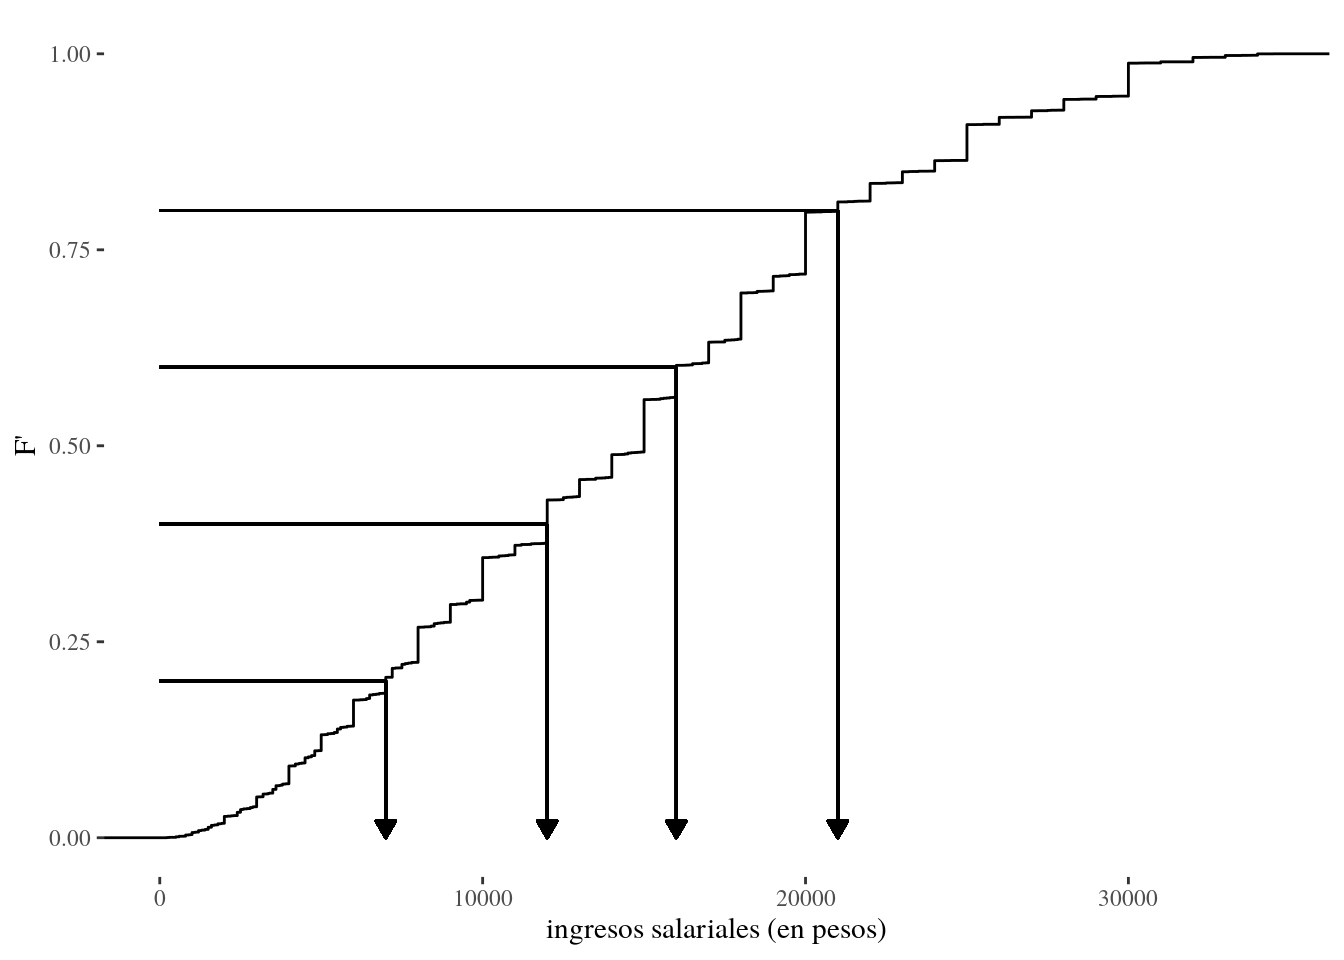
\includegraphics{EstadisticaParaCienciasSocialesConR_files/figure-latex/unnamed-chunk-64-1.pdf}

Los quintiles de esta distribución son los siguientes:

\begin{itemize}
\tightlist
\item
  \(P_{20} =\) 7000
\item
  \(P_{40} =\) 12000
\item
  \(P_{60} =\) 16000
\item
  \(P_{80} =\) 21000
\end{itemize}

Y representan valores de ingreso salarial que contienen un qunito de los asalariados cada uno.

\hypertarget{hacerlo-en-r}{%
\subsection{Hacerlo en R}\label{hacerlo-en-r}}

Los nombres de las medidas descriptivas en R están en inglés, por lo que hay que recordarlas. Para el caso de la variable ingreso salarial (\texttt{PP08D1} en los microdatos de la EPH), hemos generado una base nueva que solo contiene personas que trabajan como obreros o empleados (son asalariados), sobre ella, las medidas de posición se piden así:

\begin{Shaded}
\begin{Highlighting}[]
\KeywordTok{attach}\NormalTok{(eph.}\DecValTok{3}\NormalTok{.}\FloatTok{18.}\NormalTok{asal)}
\KeywordTok{length}\NormalTok{(PP08D1) }\CommentTok{# cantidad de casos (n)}
\end{Highlighting}
\end{Shaded}

\begin{verbatim}
## [1] 13410
\end{verbatim}

\begin{Shaded}
\begin{Highlighting}[]
\KeywordTok{mean}\NormalTok{(PP08D1) }\CommentTok{# la media}
\end{Highlighting}
\end{Shaded}

\begin{verbatim}
## [1] 14586.19
\end{verbatim}

\begin{Shaded}
\begin{Highlighting}[]
\KeywordTok{median}\NormalTok{(PP08D1) }\CommentTok{# la mediana}
\end{Highlighting}
\end{Shaded}

\begin{verbatim}
## [1] 15000
\end{verbatim}

Para los percentiles, se debe especificar cuál o cuáles \emph{cuantiles} se piden:

\begin{Shaded}
\begin{Highlighting}[]
\KeywordTok{quantile}\NormalTok{(PP08D1, }\FloatTok{.2}\NormalTok{) }\CommentTok{# percentil 20}
\end{Highlighting}
\end{Shaded}

\begin{verbatim}
##  20% 
## 7000
\end{verbatim}

\begin{Shaded}
\begin{Highlighting}[]
\KeywordTok{quantile}\NormalTok{(PP08D1, }\FloatTok{.05}\NormalTok{) }\CommentTok{# percentil 5}
\end{Highlighting}
\end{Shaded}

\begin{verbatim}
##   5% 
## 3000
\end{verbatim}

\begin{Shaded}
\begin{Highlighting}[]
\KeywordTok{quantile}\NormalTok{(PP08D1, }\FloatTok{.95}\NormalTok{) }\CommentTok{# percentil 95}
\end{Highlighting}
\end{Shaded}

\begin{verbatim}
##   95% 
## 30000
\end{verbatim}

\begin{Shaded}
\begin{Highlighting}[]
\KeywordTok{quantile}\NormalTok{(PP08D1, }\FloatTok{.5}\NormalTok{) }\CommentTok{# percentil 50, coincide con la mediana}
\end{Highlighting}
\end{Shaded}

\begin{verbatim}
##   50% 
## 15000
\end{verbatim}

Si se necesitan varios juntos, por ejemplo los quintiles, se usa el comando \texttt{c}, para ``concatenar'' los valores:

\begin{Shaded}
\begin{Highlighting}[]
\KeywordTok{quantile}\NormalTok{(PP08D1, }\KeywordTok{c}\NormalTok{(.}\DecValTok{2}\NormalTok{, }\FloatTok{.4}\NormalTok{, }\FloatTok{.6}\NormalTok{, }\FloatTok{.8}\NormalTok{))}
\end{Highlighting}
\end{Shaded}

\begin{verbatim}
##   20%   40%   60%   80% 
##  7000 12000 16000 21000
\end{verbatim}

Esta descripción de los datos se lee:
En la muestra de 13410 personas que trabajan como obreros o empleados, el salario promedio es de 14586.19. El 50\% tiene salario de 15000, el 20\% de más bajos salarios está de 7000 para abajo y el 5\% de los menores salarios son de 3000 o menos. El 95\% tiene salario de 30000 o menos; que es lo mismo que decir que el 5\% de los salarios superan los 30000.

Para realizar la categorización con los tres criterios vistos antes, se cuenta en R con la función \texttt{cut} que se aplica sobre una variable cuantitativa y se controla la cantidad de intervalos y la forma de construirlos en el argumento ``breaks''. Por ejemlo, para categorizar la edad de la base EPH en cuatro intervalos de igual amplitud, se indica ese número en el argumento. El resultado de esa categorización se guarda en una nueva variable a la que llamamos z y luego se solicita su distribución de frecuencia:

\begin{Shaded}
\begin{Highlighting}[]
\NormalTok{z <-}\StringTok{ }\KeywordTok{cut}\NormalTok{(eph.}\FloatTok{3.18}\OperatorTok{$}\NormalTok{CH06, }\DataTypeTok{breaks =} \DecValTok{4}\NormalTok{)}
\KeywordTok{table}\NormalTok{(z)}
\end{Highlighting}
\end{Shaded}

\begin{verbatim}
## z
## (-0.101,25.2]   (25.2,50.5]   (50.5,75.8]    (75.8,101] 
##         23233         18769         12342          2535
\end{verbatim}

El límite inferior del primer intervalo es negativo por la aplicación de una fórmula de cálculo de las amplitudes, cuando se edita para presentarla, ese número debe ser cero.

La otra opción del argumento ``breaks'' es indicarle un vector con los límites de los intervalos que se desea. La categorización con criterio proporcional debe indicar que los puntos de corte sean los percentiles correspondientes a la cantidad requerida, para cuatro intervalos, se indica el mínimo de la variable como inicio, luego los cuartiles y termina en el máximo:

\begin{Shaded}
\begin{Highlighting}[]
\NormalTok{t <-}\StringTok{ }\KeywordTok{cut}\NormalTok{(eph.}\FloatTok{3.18}\OperatorTok{$}\NormalTok{CH06, }\DataTypeTok{breaks =} \KeywordTok{c}\NormalTok{(}
  \KeywordTok{min}\NormalTok{(eph.}\FloatTok{3.18}\OperatorTok{$}\NormalTok{CH06),}
  \KeywordTok{quantile}\NormalTok{(eph.}\FloatTok{3.18}\OperatorTok{$}\NormalTok{CH06, }\FloatTok{.25}\NormalTok{),}
  \KeywordTok{quantile}\NormalTok{(eph.}\FloatTok{3.18}\OperatorTok{$}\NormalTok{CH06, }\FloatTok{.5}\NormalTok{),}
  \KeywordTok{quantile}\NormalTok{(eph.}\FloatTok{3.18}\OperatorTok{$}\NormalTok{CH06, }\FloatTok{.75}\NormalTok{),}
  \KeywordTok{max}\NormalTok{(eph.}\FloatTok{3.18}\OperatorTok{$}\NormalTok{CH06)}
\NormalTok{))}
\KeywordTok{table}\NormalTok{(t)}
\end{Highlighting}
\end{Shaded}

\begin{verbatim}
## t
##   (0,16]  (16,32]  (32,52] (52,101] 
##    13913    14280    14292    13673
\end{verbatim}

Con estos cortes, los grupos tienen cantidades de casos similares.

Si el criterio es teórico, se eligen los puntos de corte y se indican en ``breaks''. Para hacer cuatro grupos de: hasta 14 años, de 15 a 44, de 45 a 64 y 65 o más, se solicita:

\begin{Shaded}
\begin{Highlighting}[]
\NormalTok{u <-}\StringTok{ }\KeywordTok{cut}\NormalTok{(eph.}\FloatTok{3.18}\OperatorTok{$}\NormalTok{CH06, }\DataTypeTok{breaks =} \KeywordTok{c}\NormalTok{(}
  \KeywordTok{min}\NormalTok{(eph.}\FloatTok{3.18}\OperatorTok{$}\NormalTok{CH06),}
  \DecValTok{14}\NormalTok{,}
  \DecValTok{44}\NormalTok{,}
  \DecValTok{64}\NormalTok{,}
  \KeywordTok{max}\NormalTok{(eph.}\FloatTok{3.18}\OperatorTok{$}\NormalTok{CH06)}
\NormalTok{))}
\KeywordTok{table}\NormalTok{(u)}
\end{Highlighting}
\end{Shaded}

\begin{verbatim}
## u
##   (0,14]  (14,44]  (44,64] (64,101] 
##    12052    25333    11780     6993
\end{verbatim}

\hypertarget{la-forma-de-la-distribucion}{%
\section{La forma de la distribución}\label{la-forma-de-la-distribucion}}

La media es una medida muy completa como resumen de los datos, ya que
los considera a todos con la frecuencia de cada uno. Opera como un punto
de equilibrio en un conjunto de datos. Sin embargo esto puede ser una
dificultad en algunos tipos de distribución. Consideremos el siguiente
ejemplo simple:

\begin{longtable}[]{@{}lc@{}}
\toprule
x & f\tabularnewline
\midrule
\endhead
3 & 16\tabularnewline
4 & 7\tabularnewline
5 & 5\tabularnewline
6 & 6\tabularnewline
10 & 3\tabularnewline
Total & 37\tabularnewline
\bottomrule
\end{longtable}

Estos datos muestran una marcada concentración en el valor 3, donde se
encuentra la mitad de las observaciones. El resto de los valores son
superiores y hay uno extremo, el 10, que tiene poca frecuencia: hay solo
tres observaciones con ese valor. Veamos cuál es el efecto de esta forma
de distribuirse de los datos. La media es:

\begin{verbatim}
## [1] 4.51
\end{verbatim}

\[\overline{x} = \frac{3*16 + 4*7 + 5*5 + 6*6 + 10*3}{37} = 4.51\]

A pesar de la concentración en 3 que se observa, la media es superior a 4, que es un resultado contrario a lo que intuitivamente esperaríamos,
porque habríamos supuesto que se ubicaría más cerca de 3, ya que 3
parece ser un valor muy ``representativo'' de esta distribución, sin
embargo, la media da un número bastante más grande. Esto se debe a la
presencia de valores extremos, en este ejemplo el 10. Aunque este número
tiene poca frecuencia, su efecto es de ``tirar de la media'' hacia valores
más grandes. Esto sucede siempre con la media y proviene de su
característica de tener en cuenta todos los valores de la distribución.
Por esa razón, cuando la distribución se presenta como la anterior, la
media no es una buena medida de centralidad.

Este inconveniente de la media aparece a menudo en las discusiones
salariales por sectores. A menudo se escucha que no se justifica un
aumento porque el salario promedio de todos los empleados del sector es
de \emph{X pesos}. Argumento al que se contrapone (expresado de diferentes
maneras) que ese promedio incluye al personal que tiene salarios muy
altos. Se trata de distribuciones asimétricas, que tienen la mayor parte
de los casos con salarios bajos o intermedios y unos pocos casos con
salarios muy superiores, por eso cuando se calcula la media se obtiene
un resultado que representa mal al conjunto de datos.

El histograma siguiente muestra la forma de la distribución anterior:

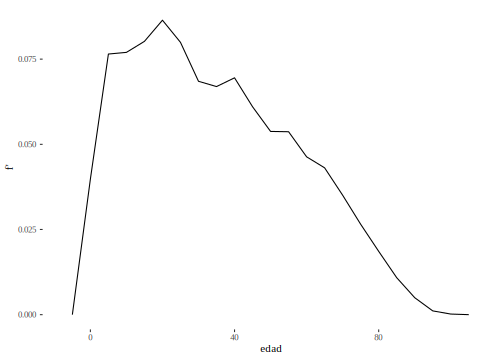
\includegraphics{EstadisticaParaCienciasSocialesConR_files/figure-latex/unnamed-chunk-74-1.pdf}

En el gráfico se ve el carácter atípico del valor 10, que aparece muy
alejado de la parte principal de la distribución. Decimos en este caso
que la distribución es asimétrica.

\hypertarget{asimetria}{%
\subsection{Asimetría}\label{asimetria}}

La \textbf{asimetría} de una distribución se indica señalando hacia dónde se
sitúan los valores extremos. Si, como en este ejemplo, los valores
extremos son mayores que la mayor parte de los datos, la asimetría es
\textbf{hacia la derecha}.

La asimetría puede ser en sentido opuesto, si hay observaciones
particularmente pequeñas y en ese caso se tratará de una distribución
\textbf{asimétrica hacia la izquierda}. Como en el ejemplo siguiente:

\begin{longtable}[]{@{}lc@{}}
\toprule
X & F\tabularnewline
\midrule
\endhead
100 & 5\tabularnewline
200 & 10\tabularnewline
300 & 20\tabularnewline
400 & 20\tabularnewline
500 & 50\tabularnewline
600 & 70\tabularnewline
Total & 175\tabularnewline
\bottomrule
\end{longtable}

Cuyo histograma es:

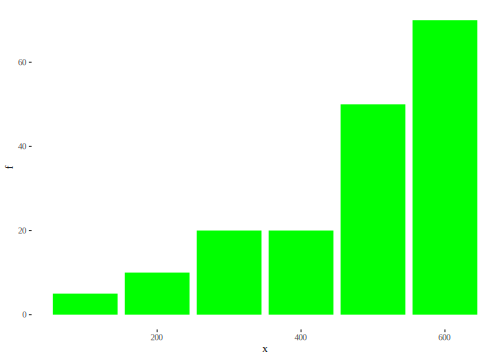
\includegraphics{EstadisticaParaCienciasSocialesConR_files/figure-latex/unnamed-chunk-76-1.pdf}

Aquí los valores extremos se encuentran por debajo del grupo principal
de datos y la media se inclinará hacia los valores más pequeños. Así,
aunque la mayoría de los casos se encuentra entre 500 y 600, la media
es:

\begin{verbatim}
## [1] 477.14
\end{verbatim}

\[\overline{x} = \frac{100*5 + 200*10 + 300*20 + 400*20 + 500*50 + 600*70}{175} = 477,14\]

Un resultado que está por debajo de esos valores que concentran muchos
casos. Decimos ahora que la asimetría es hacia la izquierda.

Los siguientes histogramas, son ejemplos de formas posibles en cuanto a simetría:

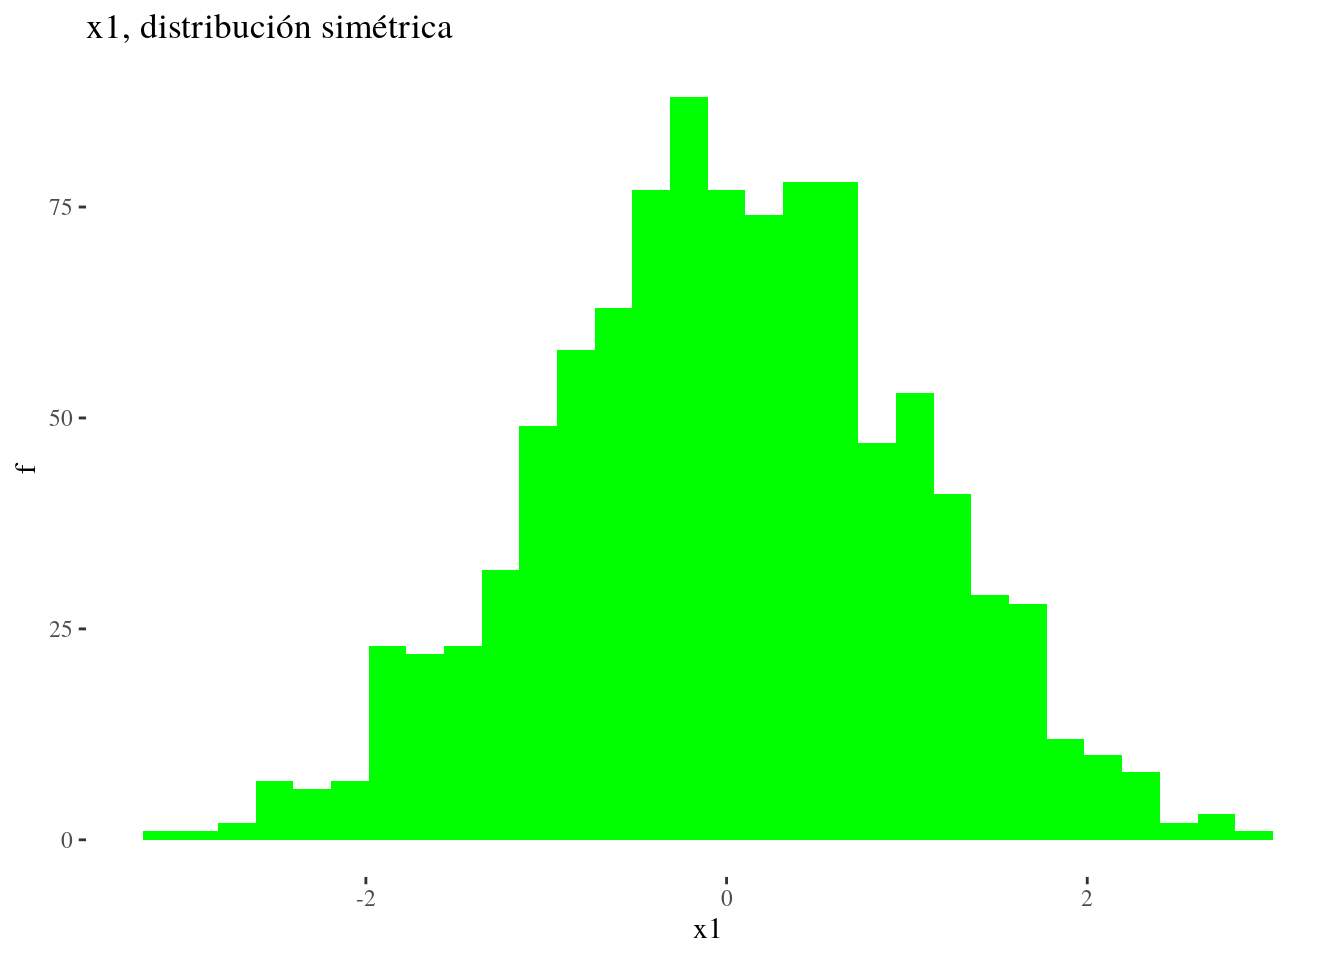
\includegraphics{EstadisticaParaCienciasSocialesConR_files/figure-latex/unnamed-chunk-78-1.pdf} 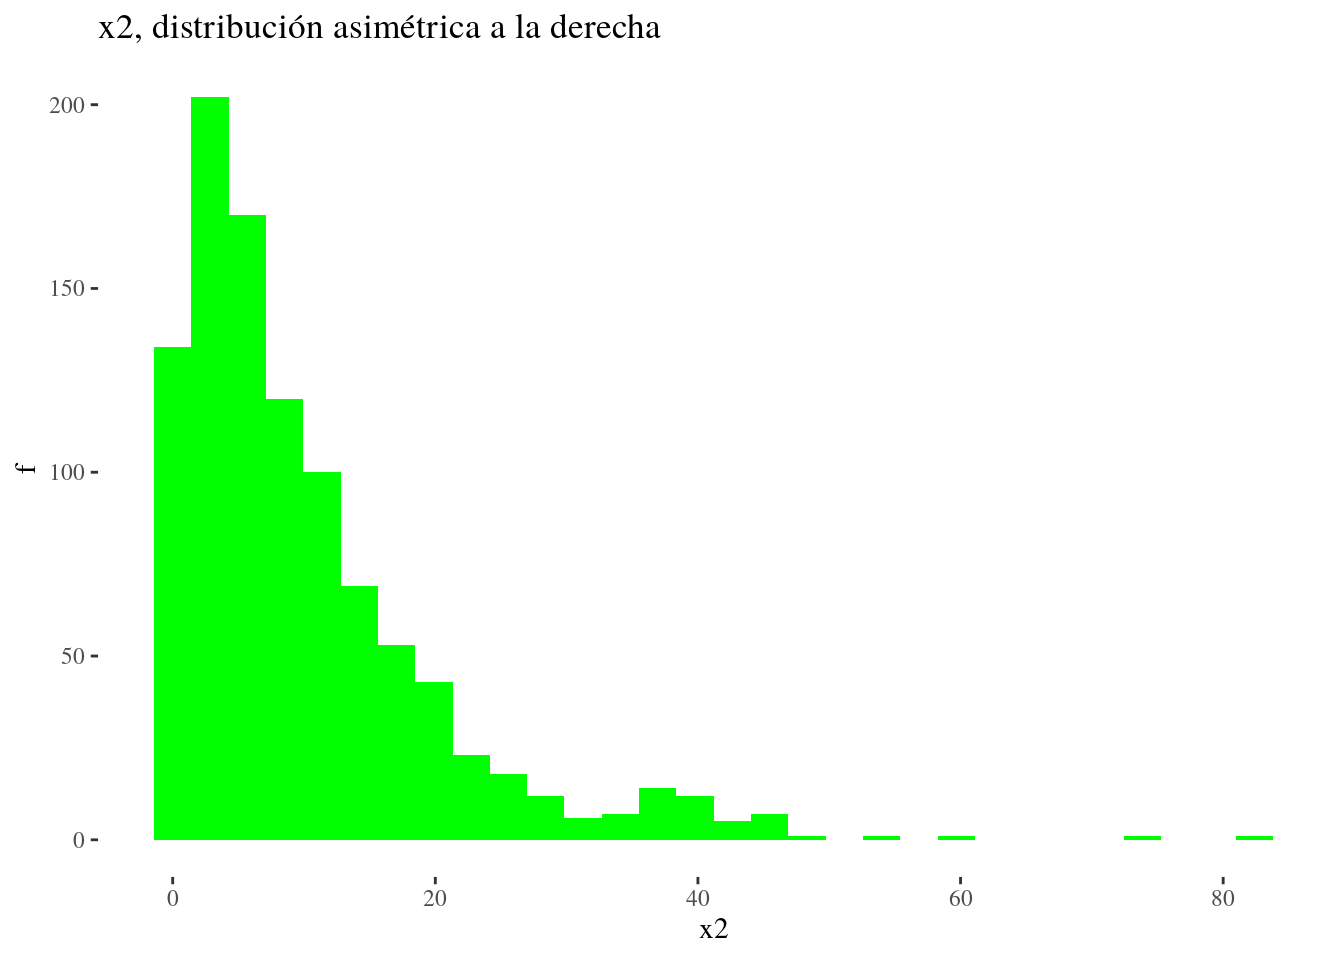
\includegraphics{EstadisticaParaCienciasSocialesConR_files/figure-latex/unnamed-chunk-78-2.pdf} 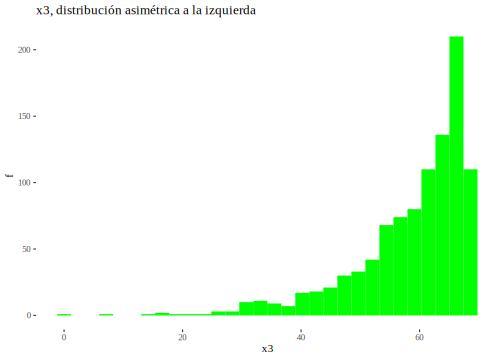
\includegraphics{EstadisticaParaCienciasSocialesConR_files/figure-latex/unnamed-chunk-78-3.pdf}

La asimetría puede evaluarse directamente a partir de las medidas de
centralidad, ya que la posición relativa de la media y la mediana
indican hacia dónde ésta sucede. Cuando la media y la mediana coinciden,
la distribución es simétrica, es decir carece de asimetría. Si la media
supera a la mediana, se trata de una distribución asimétrica a la
derecha y si la media es menor que la mediana, la asimetría será hacia
la izquierda.

En estas distribuciones las medias y medianas son:

\begin{itemize}
\tightlist
\item
  x1: media = -0.0551901, mediana = -0.0270521
\item
  x2: media = 10.1045686, mediana = 7.0312563
\item
  x3: media = 9.8993681, mediana = 9.6869492
\end{itemize}

\begin{longtable}[]{@{}cc@{}}
\toprule
Posición relativa de la media y la mediana: & Asimetría de la Distribución:\tabularnewline
\midrule
\endhead
\(\overline{x} = M_{dn}\) & Simétrica\tabularnewline
\(\overline{x} > M_{dn}\) & Asimétrica a la derecha\tabularnewline
\(\overline{x} < M_{dn}\) & Asimétrica a la izquierda\tabularnewline
\bottomrule
\end{longtable}

\begin{longtable}[]{@{}c@{}}
\toprule
\endhead
\begin{minipage}[t]{0.97\columnwidth}\centering
Una distribución es \textbf{simétrica} si la media coincide con la mediana. La distribución se llama asimétrica a la derecha si la media es mayor que la mediana, y asimétrica a la izquierda si la media es menor que la mediana.\strut
\end{minipage}\tabularnewline
\bottomrule
\end{longtable}

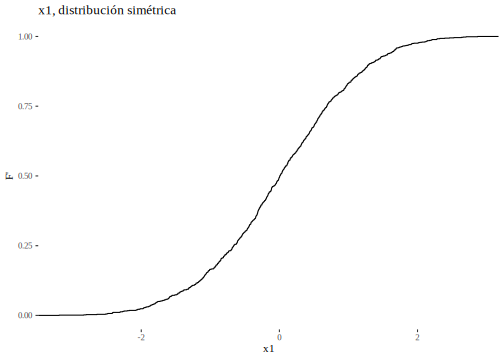
\includegraphics{EstadisticaParaCienciasSocialesConR_files/figure-latex/unnamed-chunk-79-1.pdf} 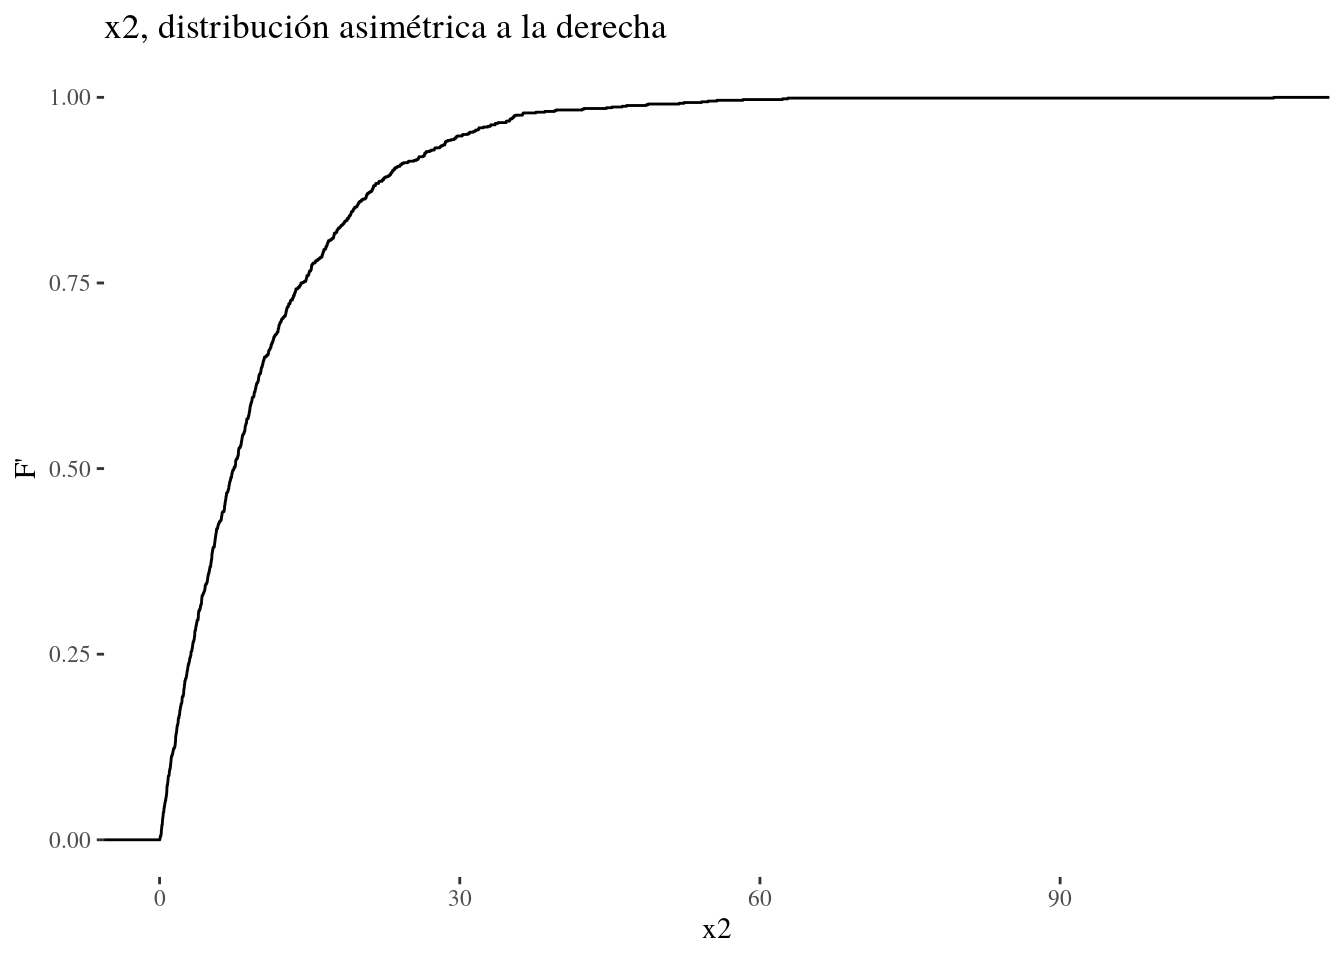
\includegraphics{EstadisticaParaCienciasSocialesConR_files/figure-latex/unnamed-chunk-79-2.pdf} 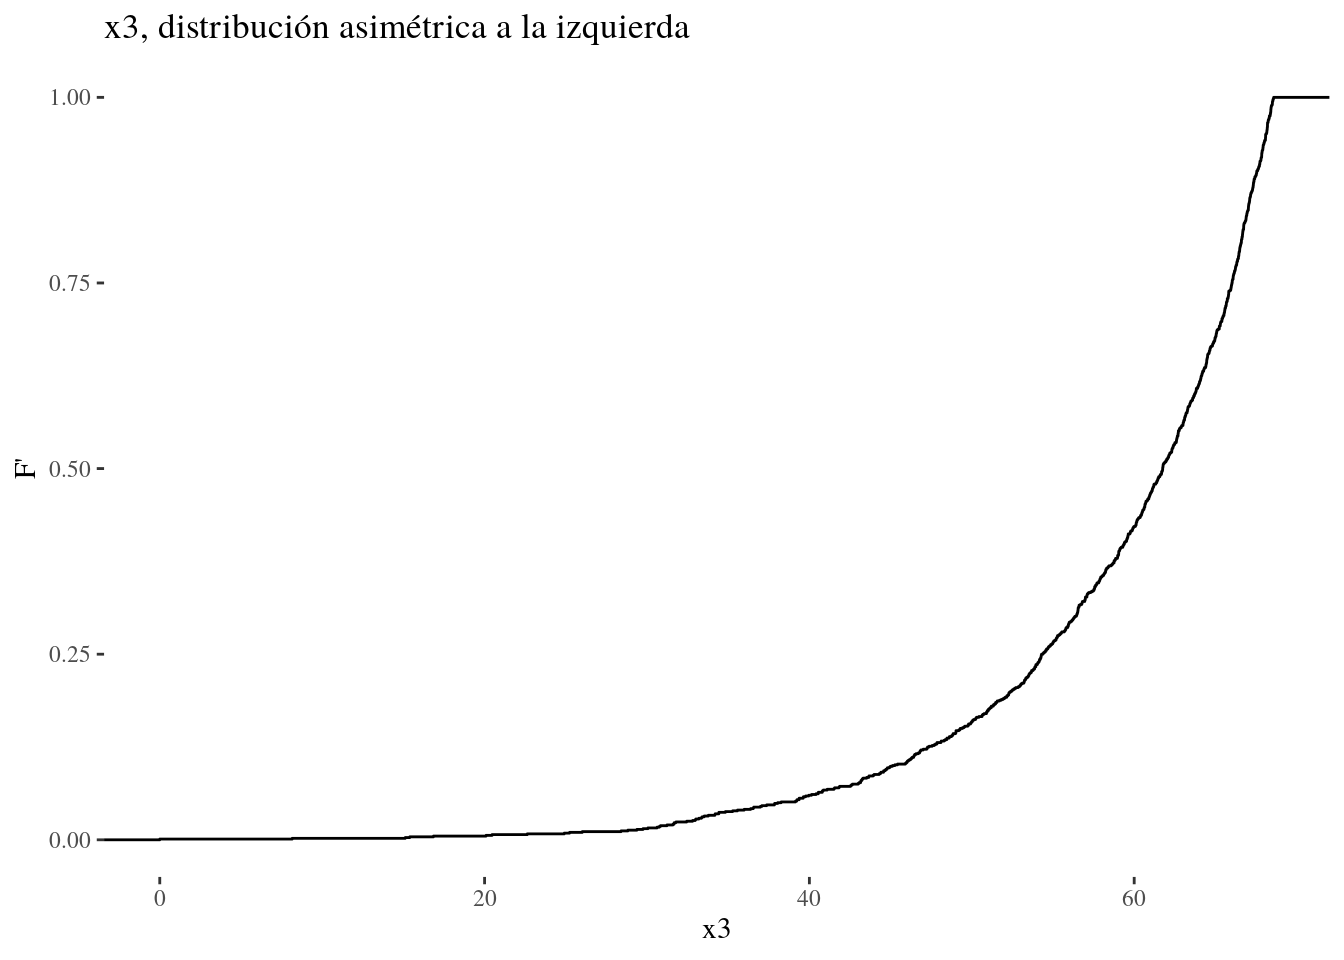
\includegraphics{EstadisticaParaCienciasSocialesConR_files/figure-latex/unnamed-chunk-79-3.pdf}

La evaluación cuantitativa de la asimetría de una distribución permite la comparación entre distribuciones en cuanto al grado de asimetría, para indicar cuando una distribución es más asimétrica que otra. Para hacerlo se usan los \emph{coeficientes de asimetría}. Estos coeficientes miden dos aspectos
de la asimetría: hacia qué lado sucede y cuán acentuada es. Su signo
positivo indica asimetría hacia la derecha y negativo hacia la
izquierda. El valor absoluto del coeficiente indica si es muy asimétrica
o poco. Por ejemplo, una distribución cuya asimetría vale 1,5 es más
asimétrica que una con coeficiente 1,2, y ambas son asimétricas hacia la
derecha. Cuando la distribución es simétrica, el coeficiente vale cero,
no es positivo ni negativo. Uno de los más frecuentemente usados es el
coeficiente de asimetría de Fisher{[}\^{}18{]}, que se calcula como:

\[g_{1} = \frac{\sum_{i = 1}^{n}{\left( x_{i} - \overline{x} \right)^{3}*f_{i}}}{n*s^{3}}\]

Y cuya interpretación es:

\begin{itemize}
\item
  \(g_{1} = 0\) La distribución es simétrica.
\item
  \(g_{1} > 0\) Asimétrica hacia la derecha.
\item
  \(g_{1} < 0\) Asimétrica hacia la izquierda.
\end{itemize}

En la práctica, es improbable que el coeficiente valga exactamente cero,
por lo que se considera simétrica a una distribución cuyo coeficiente
esté entre -0,5 y 0,5.

\hypertarget{curtosis}{%
\subsection{Curtosis}\label{curtosis}}

Además de la simetría, disponemos de otro indicador de la forma de la
distribución, una medida de cuán ``puntiaguda'' es la curva, se denomina
curtosis y distingue distribuciones con forma estrecha y elevada de que
tienen forma amplia y baja. Como en los siguientes gráficos:

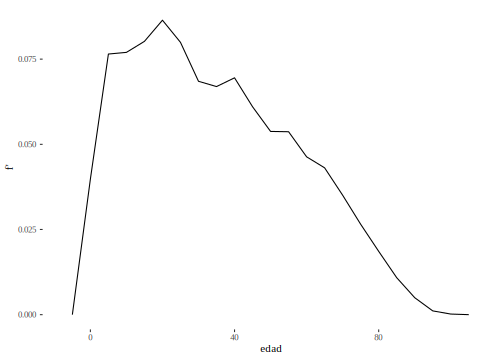
\includegraphics{EstadisticaParaCienciasSocialesConR_files/figure-latex/unnamed-chunk-80-1.pdf} 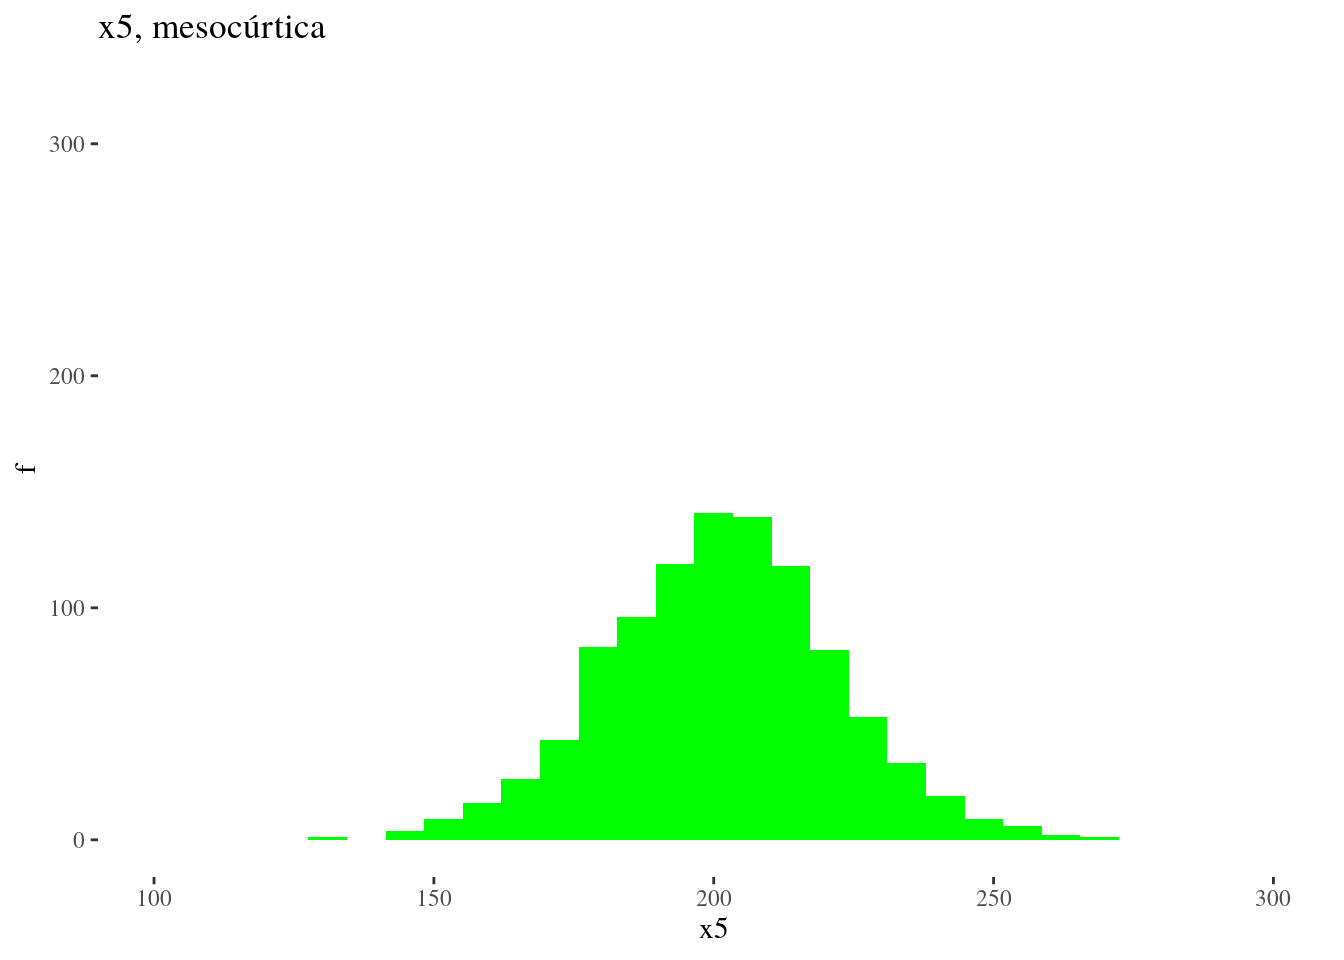
\includegraphics{EstadisticaParaCienciasSocialesConR_files/figure-latex/unnamed-chunk-80-2.pdf} 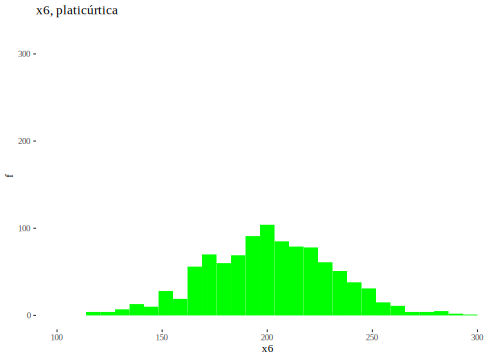
\includegraphics{EstadisticaParaCienciasSocialesConR_files/figure-latex/unnamed-chunk-80-3.pdf}

Estos tres ejemplos corresponden a distribuciones simétricas, pero
también pueden ser asimétricas.

La curtosis se mide con un coeficiente específico, que vale cero para
distribuciones mesocúrticas, es negativo para las platicúrticas y
positivo para las leptocúrticas. Su cálculo es:

\[g_{2} = \frac{\sum_{i = 1}^{n}{\left( x_{i} - \overline{x} \right)^{4}*f_{i}}}{n*s^{4}} - 3\]

Su interpretación es:

\begin{itemize}
\item
  \(g_{2} = 0\) La distribución es mesocúrtica
\item
  \(g_{2} > 0\) Leptocúrtica
\item
  \(g_{2} < 0\) Platicúrtica
\end{itemize}

Con datos reales, muy raramente el valor será exactamente cero, por lo
que se trata como mesocúrtica a una distribución cuyo coeficiente se
encuentre entre -0,5 y 0,5.

\hypertarget{box-plots}{%
\section{Box-plots}\label{box-plots}}

Un gráfico que puede resumir de manera muy compacta la información sobre
una distribución de frecuencias es el que se llama \textbf{diagrama de caja},
o también \textbf{diagrama de caja y bigotes} o \textbf{box-plot}, que fue
propuesto por John Tukey en 1977.
Aplicado a las edades de estudiantes universitarios de la EPH genera:

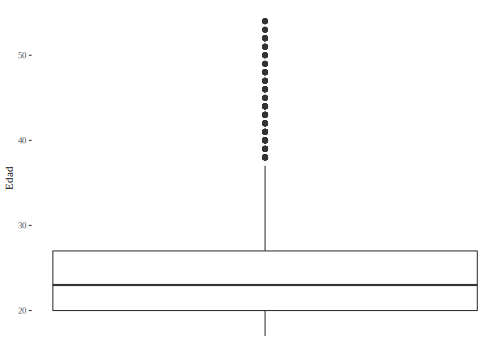
\includegraphics{EstadisticaParaCienciasSocialesConR_files/figure-latex/unnamed-chunk-81-1.pdf}

Este gráfico representa sobre el eje vertical los valores de la variable y muestra una ``caja'' delimitada por los cuartiles 1 y 3. Según la definición de los cuartiles, esa caja contiene al 50\% central de los casos. Dentro de la caja se muestra la mediana en la línea horizontal. Se aprecia la concentración de casos en los valores bajos de la variable y unos pocos casos extremos que acusan la asimetría hacia la derecha de la distribución.

El box-plot es adecuado para comparar grupos, en este ejemplo, se puede incluir la condición de actividad de los estudiantes y obtener:

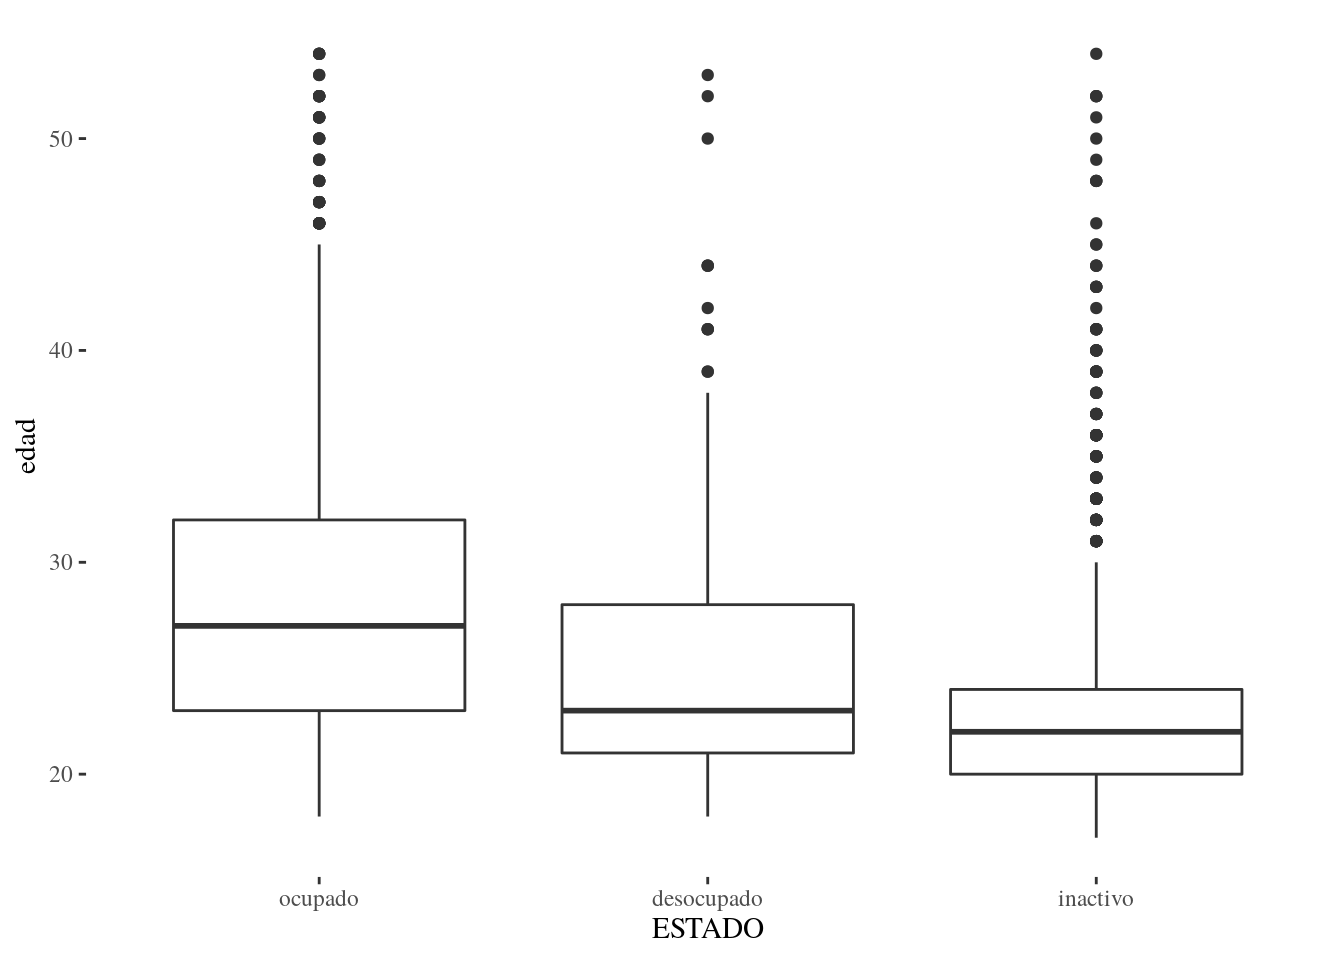
\includegraphics{EstadisticaParaCienciasSocialesConR_files/figure-latex/unnamed-chunk-82-1.pdf}

Se observa que, aunque en todos los grupos hay estudiantes con edades altas, los inactivos (que no trabajan ni buscan trabajo) son los que se concentran en la edades más bajas.

Además de la caja, se ven dos segmentos que se extienden hasta los
valores máximo y mínimo de la distribución. La longitud de estos segmentos (llamados a veces ``bigotes'') depende de una caracteírística de la distribución que se trata en el apartado siguiente: la
dispersión.

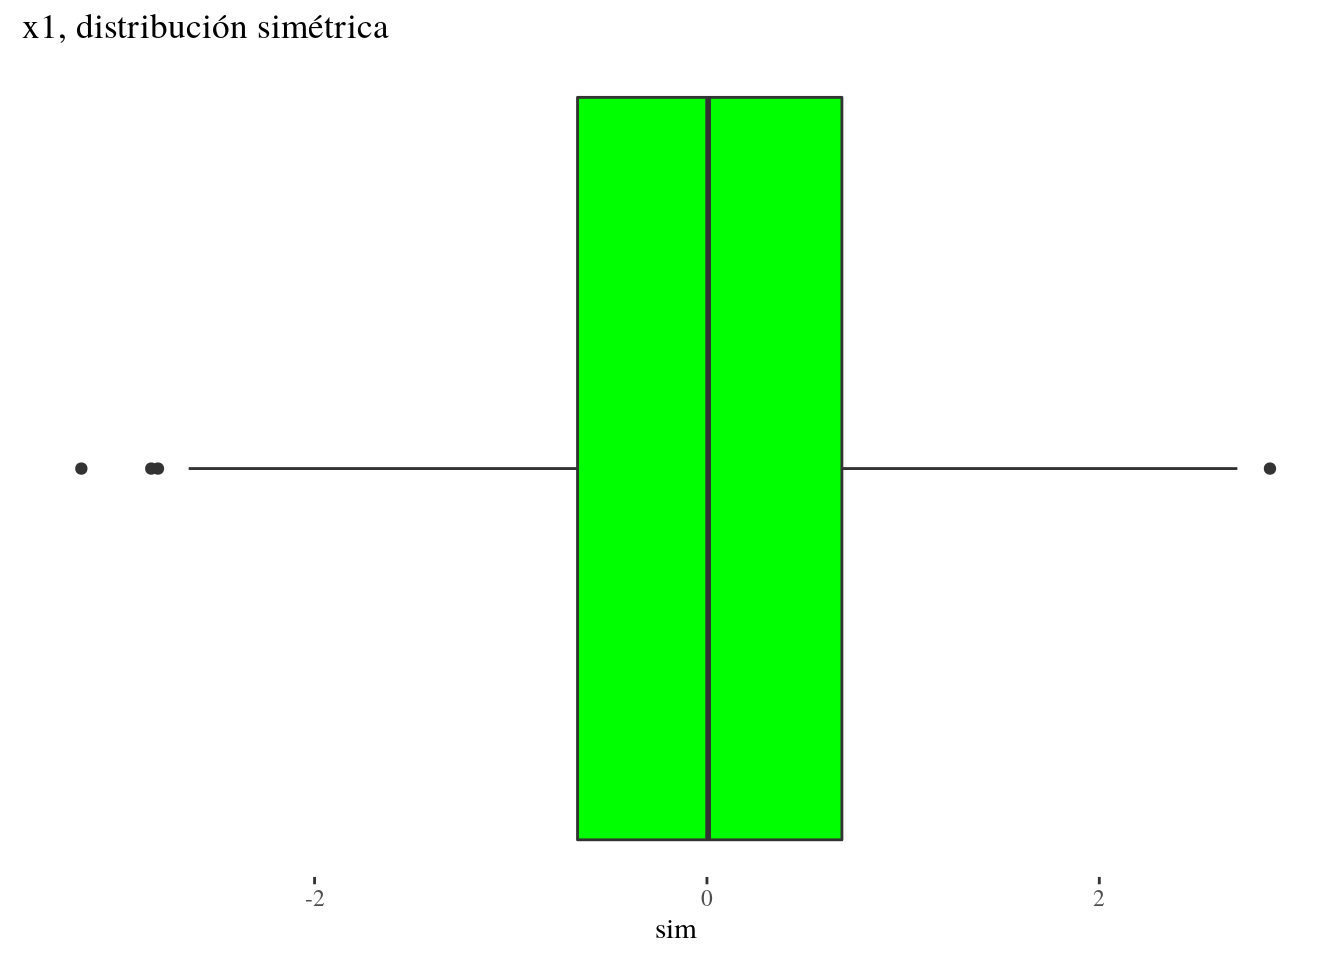
\includegraphics{EstadisticaParaCienciasSocialesConR_files/figure-latex/unnamed-chunk-83-1.pdf} 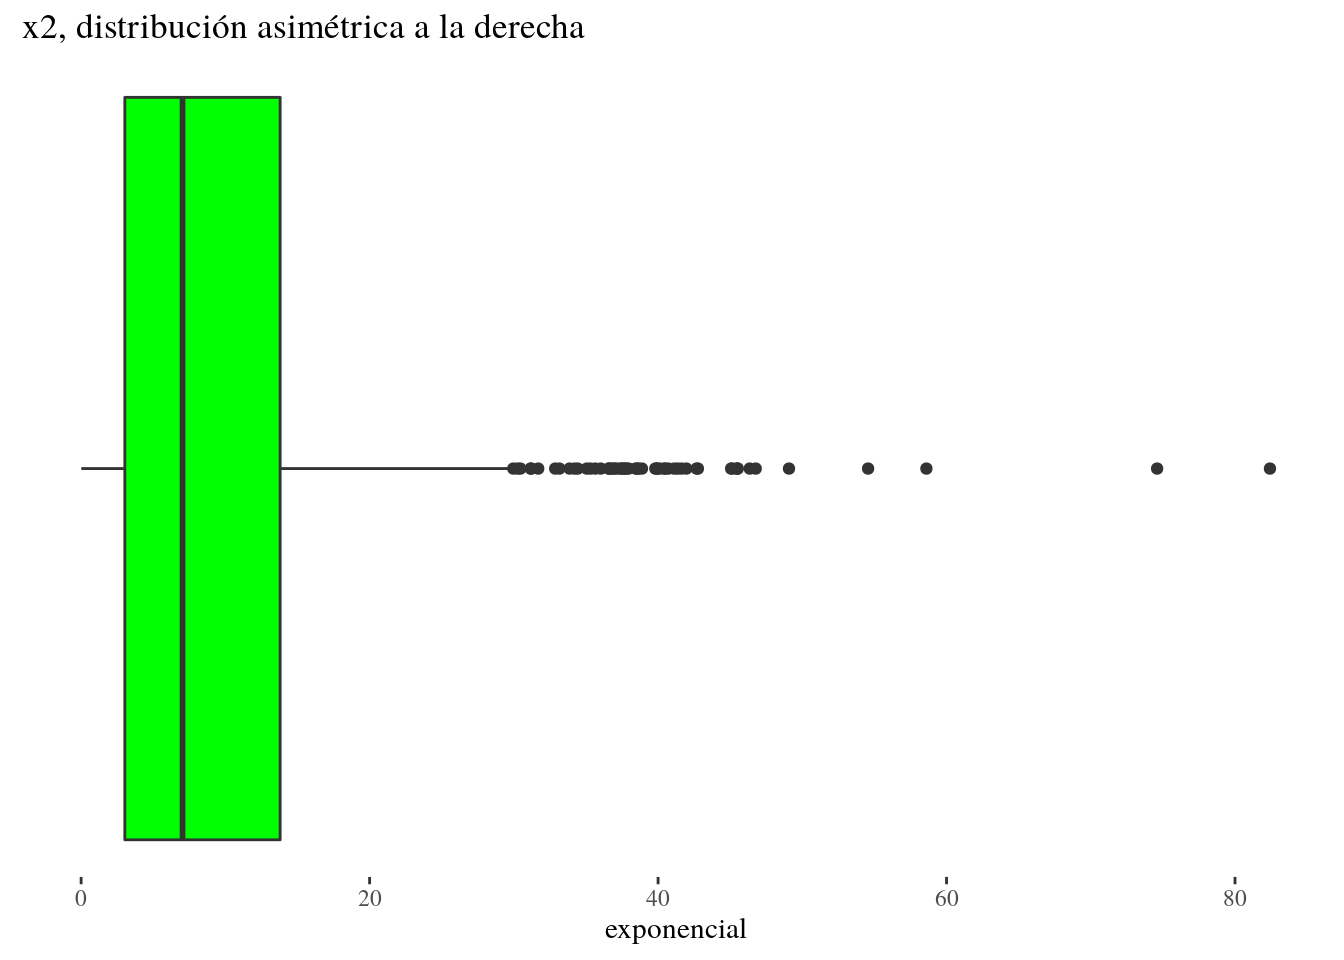
\includegraphics{EstadisticaParaCienciasSocialesConR_files/figure-latex/unnamed-chunk-83-2.pdf} 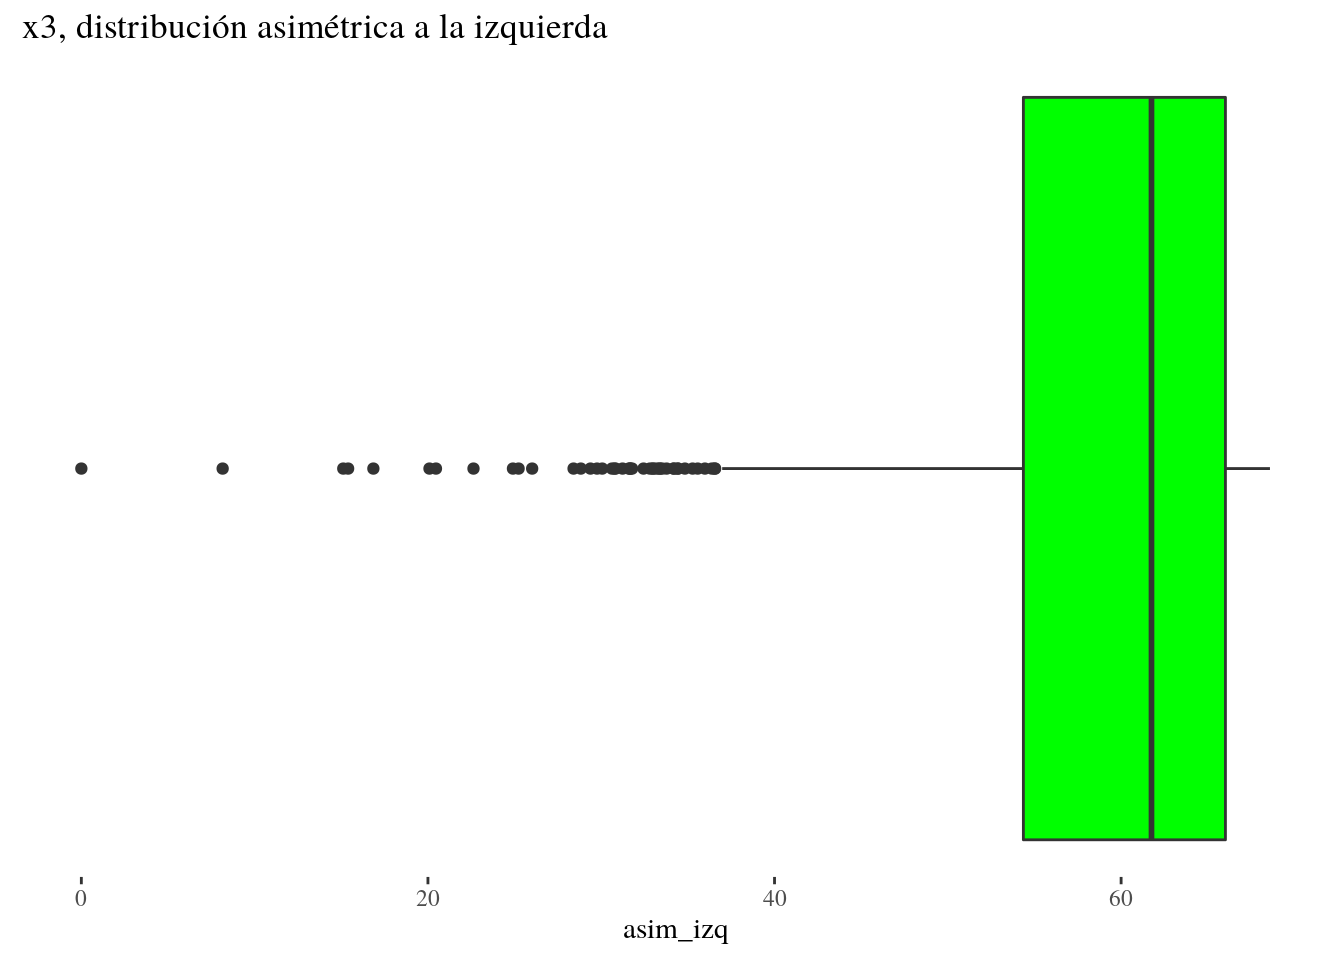
\includegraphics{EstadisticaParaCienciasSocialesConR_files/figure-latex/unnamed-chunk-83-3.pdf}

\hypertarget{medidas-de-dispersion}{%
\section{Medidas de dispersión}\label{medidas-de-dispersion}}

Además de indicar alrededor de qué valores se distribuyen los datos,también es necesario indicar si se encuentran concentrados alrededor deesos valores (si son cercanos a ellos) o dispersos (si están alejados).Por ejemplo, un promedio de 20 sesiones de psicoterapia puede provenir de cuatro casos que utilizaron 18, 19, 21 y 22 sesiones o de otros cuatro que hayan insumido 5, 10, 30 y 35 sesiones. En la primer situación las cuatro observaciones son cercanas entre sí, están concentradas, mientras que en la segunda están lejos, dispersas. Diremos que en el primer caso la distribución es homogénea o que presenta poca dispersión y en el segundo que es heterogénea o que presenta mucha dispersión.

Conocer esto tiene importancia para poder evaluar la calidad de las medidas de centralidad, en particular de la media. Esto es así porque en una distribución muy dispersa, la media será un promedio de valores muy diferentes entre sí y no será tan fiel a los datos como si estos valores fueran similares. La media de 20 sesiones del primer ejemplo es una mejor medida resumen que la misma media de 20 del segundo, porque la primera representa mejor los datos de origen. Debido a esto, decimos que en la primera de las situaciones del ejemplo, la media es más \emph{representativa} de los datos de los que proviene.

Nos ocuparemos ahora del modo en que puede medirse esa dispersión, cómo transformarla en una medida resumen que indique brevemente si los datos están dispersos o concentrados.

\hypertarget{recorrido}{%
\subsection{Recorrido}\label{recorrido}}

Una primera aproximación al problema es la de considerar la distancia que hay entre los valores extremos, entre el más pequeño y el más grande. Si usamos este procedimiento en el ejemplo anterior vemos que en la primera distribución hay 4 unidades entre la primera y la última observación (de 18 a 22) y en la segunda hay 30 unidades de extremo a extremo (de 5 a 35). Por lo que ésta sería una medida de la dispersión.
Esta medida se llama recorrido, se indica con la letra \(R\) y la expresión formal de su cálculo es:

\[R = x_{\max} - x_{\min}\]

Donde \(x_{\max}\) y \(x_{\min}\) representan a los valores máximo y mínimo
respectivamente. En las distribuciones del ejemplo, los recorridos son
\(R=4\) y \(R=30\) respectivamente, que resumen la mayor dispersión de la
segunda.

\begin{longtable}[]{@{}c@{}}
\toprule
\endhead
\begin{minipage}[t]{0.97\columnwidth}\centering
Se llama \textbf{recorrido} de una distribución a la diferencia entre los valores máximo y mínimo de la variable. Se indica \(R\).\strut
\end{minipage}\tabularnewline
\bottomrule
\end{longtable}

Cuando la distribución tiene más casos, el recorrido es insuficiente
como medida de dispersión, ya que está determinado solo por los valores
extremos. Por ejemplo, las dos siguientes series tienen la misma media,
igual a 8:

\[2, 8, 8, 8, 8, 8, 14\]

7, 8, 8, 8, 8, 8, 9

El recorrido vale 12 para la primera (\(R=14–2\)) y 2 para la segunda
(\(R=9–7\)) es una diferencia muy acentuada aunque las dos distribuciones
solo difieren en los valores extremos. Dicho de otra manera, si sucede
que hay un caso (o unos pocos) que tiene un valor excepcionalmente alto
(o bajo), el recorrido dará un valor alto, indicando gran dispersión, lo
que nos puede hacer pensar que todos los datos están dispersos. Por esa
razón se dice que es una medida ``gruesa'' de la variabilidad de los
datos.

\hypertarget{amplitud-intercuartilica}{%
\subsection{Amplitud intercuartílica}\label{amplitud-intercuartilica}}

Un modo de afinar la calidad de esta medida es la de tomar la distancia
que hay, no ya entre los valores extremos, sino entre los cuartiles
primero y tercero. La medida que usa esta distancia se llama amplitud
intercuartílica y es simplemente la diferencia entre el tercer cuartil y
el primero:

\[AIQ = Q_{3}{- Q}_{1}\]

Si bien tampoco es ésta una medida que considere todas las observaciones
-ya que solo tiene en cuenta los dos cuartiles-, es mejor que el
recorrido, porque deja de lado los valores extremos, aquellos que
pertenecen al 25\% más bajo y al 25\% más alto de la distribución.

\begin{longtable}[]{@{}c@{}}
\toprule
\endhead
\begin{minipage}[t]{0.97\columnwidth}\centering
La \textbf{amplitud intercuartílica} es la diferencia entre los cuartiles tercero y primero. Se indica \(AIQ\).\strut
\end{minipage}\tabularnewline
\bottomrule
\end{longtable}

Gráficamente, esta medida es la altura de la caja del Box-plot. Algunos autores prefieren informar como medida de dispersión a la mitad de la distancia entre los cuartiles 1 y 3, a la que se denomina \emph{semi recorrido intercuartilar}, y se abrevia SRIC. No tiene diferencia conceptual con la AIQ, porque ambas consideran distancia entre cuartiles, solo difieren en la convención de informar la distancia completa (AIC) o su mitad (SRIC).

\begin{longtable}[]{@{}c@{}}
\toprule
\endhead
\begin{minipage}[t]{0.97\columnwidth}\centering
El \textbf{semi recorrido intercuartilar} es la mitad de la amplitud intercuartílica. Se indica \(SRIC\).\strut
\end{minipage}\tabularnewline
\bottomrule
\end{longtable}

Que en el Box-plot representa al mitad de la altura de la caja.

\[SRIC = \frac{Q_{3}{- Q}_{1}}{2}\]

\hypertarget{medidas-de-dispersion-basadas-en-la-media}{%
\subsection{Medidas de dispersión basadas en la media}\label{medidas-de-dispersion-basadas-en-la-media}}

Las medidas de variabilidad que más se usan son las que tienen en cuenta
todas las observaciones, es decir aquellas que están basadas en la
media. Una manera de ver si el conjunto de datos está concentrado o
disperso, consiste en observar la distancia de la media a la que se
encuentra cada observación, luego esas distancias individuales pueden
promediarse y tener una idea global de qué tan lejos están los casos del
promedio. Intentemos hacer eso y veamos qué limitación aparece.

Tomemos un conjunto pequeño de datos, presentado en serie simple:

\[5, 7, 9, 11\]

La media es 8, como lo es la mediana. Aunque no hay modo, ya que todos
los valores tienen frecuencia igual a uno, la distribución es simétrica.
Hemos elegido así el ejemplo solo para darle simplicidad, no es una
condición necesaria para lo que sigue.

Consideremos las distancias desde cada observación hasta la media,
restando a cada una de ellas el valor 8 (la media):

\begin{longtable}[]{@{}cc@{}}
\toprule
\(x_{i}\) & \(x_{i} - \overline{x}\)\tabularnewline
\midrule
\endhead
5 & -3\tabularnewline
7 & -1\tabularnewline
9 & 1\tabularnewline
11 & 3\tabularnewline
\bottomrule
\end{longtable}

Las distancias positivas corresponden a valores superiores a la media y
las negativas a los inferiores, si un valor acertara en la media, su
distancia sería cero. Si sumamos todas las diferencias
\(x_{i} - \overline{x}\), el resultado es cero (\(-3-1+1+3=0\)); además, éstas
son simétricas, como efecto de la forma de la distribución original.
Pero el hecho que la suma sea cero no depende de la distribución, sino que es una propiedad de la media. Por ser la media un punto de equilibrio entre las observaciones, las que se distancian por
encima de ella están compensadas por las que lo hacen por debajo.

Los valores \(x_{i} - \overline{x}\) se llaman desvíos, que indican cuánto
se aleja cada observación de la media. Como vemos pueden ser positivos o
negativos según se trate de observaciones que superen a la media o que
estén por debajo de ella. Acabamos de ver también que su suma vale cero,
es decir que \(\sum_{i = 1}^{n}{\left( x_{i} - \overline{x} \right) = 0}\)
y que esta es una cualidad de la media, que no depende de los
datos.

La representación gráfica de esta propiedad puede verse pensando en una analogía física; como si cada caso graficado en el histograma fuese un bloque de ciert0, situado en el valor de la variable. Con esa idea, la ubicación de la media es el punto donde habria que apoyar el histograma para que éste quede en equilibrio:

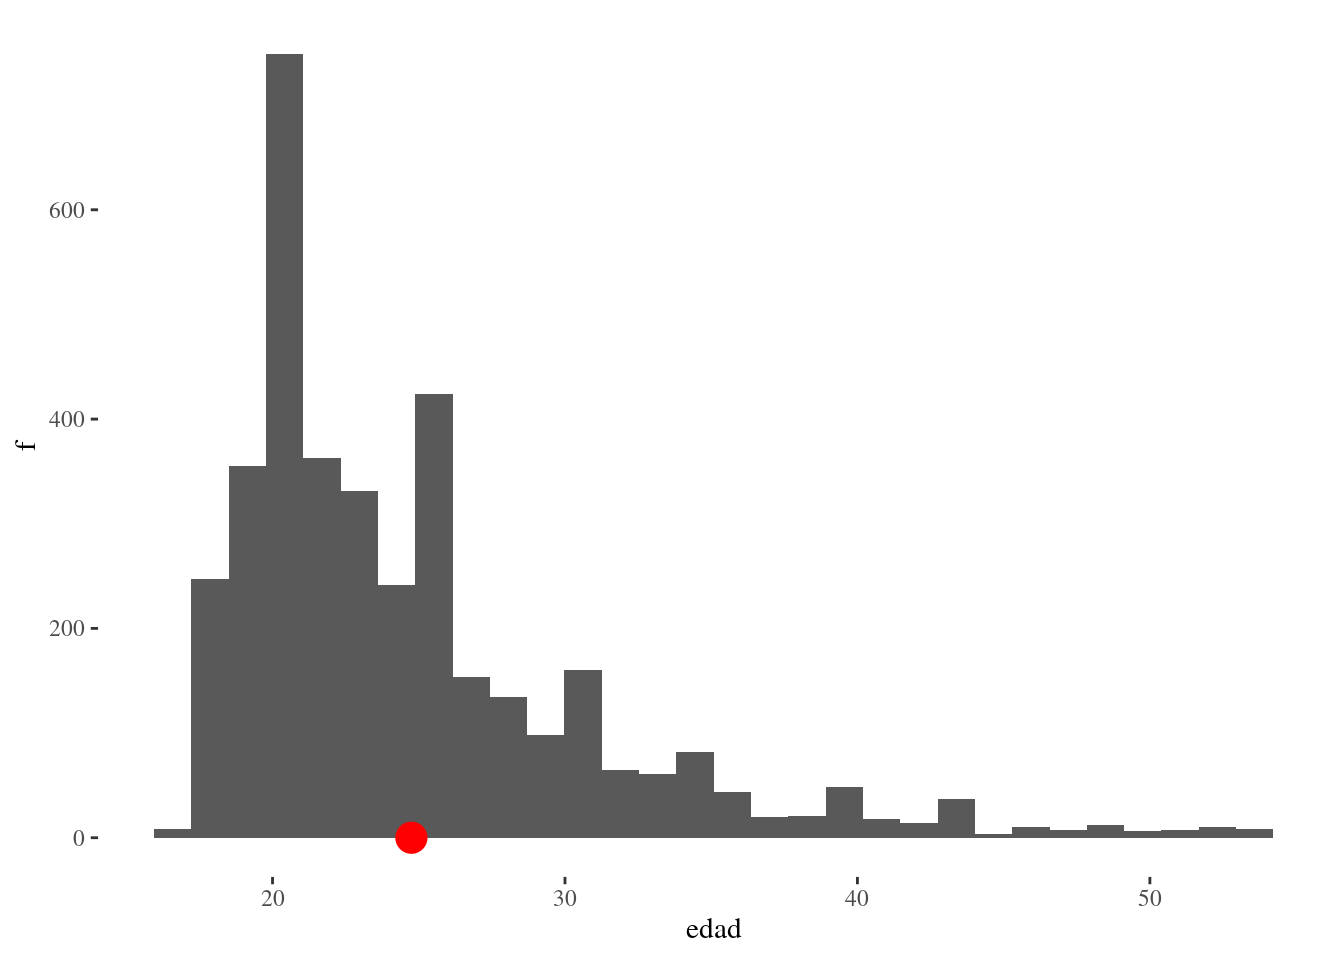
\includegraphics{EstadisticaParaCienciasSocialesConR_files/figure-latex/unnamed-chunk-84-1.pdf}

El punto (triángulo) del gráfico equivale al punto de apoyo que permite el equilibrio de ese ``objeto''.

Tan importante es esta propiedad que la usaremos para dar
una definición más completa de la media:

\begin{longtable}[]{@{}c@{}}
\toprule
\endhead
\begin{minipage}[t]{0.97\columnwidth}\centering
La \textbf{media} es el valor de la variable que anula la suma de los desvíos en torno suyo.\strut
\end{minipage}\tabularnewline
\bottomrule
\end{longtable}

El tema que nos ocupa en este momento, es el de medición de la
variabilidad del conjunto de casos, y entonces, la consecuencia de esta propiedad es que no será posible usar la suma de los desvíos como indicador de dispersión, ya que da siempre cero, con datos homogéneos o heterogéneos.

A fin de resolver este problema vamos a eliminar el signo, usando el
hecho que todo número elevado a una potencia par es positivo, sin
importar el signo que haya tenido el número. Elevaremos entonces al
cuadrado cada una de los desvíos y así se perderá su signo y ya no será cero la suma de todos ellos.

\hypertarget{varianza}{%
\subsection{Varianza}\label{varianza}}

Usando ese recurso, definimos la varianza, a la que simbolizaremos como \(V(x)\) o más frecuentemente como \(s^2\) de la siguiente forma:

\[s^{2} = \frac{\sum_{i = 1}^{n}\left( x_{i} - \overline{x} \right)^{2}}{n - 1}\]

\begin{longtable}[]{@{}c@{}}
\toprule
\endhead
\begin{minipage}[t]{0.97\columnwidth}\centering
Se llama \textbf{varianza} de una distribución a la suma de los cuadrados de los desvíos alrededor de la media, dividida por el total de observaciones menos uno. Se indica \(s^2\).\strut
\end{minipage}\tabularnewline
\bottomrule
\end{longtable}

Es una medida muy valiosa de la dispersión que tiene un conjunto de
datos, cuanto mayor es, tanto más dispersos éstos se encuentran, es
decir, son más heterogéneos. No puede ser negativa, porque es una suma de cuadrados y solo es cero si todos los desvíos son cero, es decir si todas las observaciones coinciden con la media.

Hay tres propiedades de la varianza que señalaremos porque serán
necesarias más adelante:

-La varianza de una constante es cero. Esto resulta claro ya que la
varianza mide la dispersión y si todas las observaciones son iguales no hay dispersión:

\[V\left( k \right) = 0\]

-La varianza de una constante que multiplica a una variable es la
constante elevada al cuadrado multiplicada por la varianza de la
variable:

\[V\left( k*x \right) = k^{2}*V(x)\]

-La varianza de la suma de dos variables independientes es la suma de
las varianzas de cada una de ellas:

\[V\left( x + y \right) = V\left( x \right) + V(y)\]

A los fines de la interpretación, la varianza presenta dos
inconvenientes. Uno es que sus unidades están elevadas al cuadrado; por lo que, si medimos \emph{número de errores}, la varianza quedará expresada en \emph{número de errores al cuadrado} una entidad que no tiene significado, como tampoco lo tienen \emph{hijos al cuadrado} para la fecundidad, \emph{pesos al cuadrado} para ingresos o \emph{segundos al cuadrado} para los tiempos de reacción.

El otro inconveniente es que no tiene límite superior, puede ser muy
grande y no tenemos con qué compararla para saber si indica una gran
variabilidad o si es grande porque los valores de la variable lo son.

\hypertarget{desviacion-estandar}{%
\subsection{Desviación estándar}\label{desviacion-estandar}}

Para resolver el primer inconveniente, definiremos una medida derivada de la varianza, que se denomina desviación estándar (en algunos textos y programas de análisis de datos es llamada desviación típica). Esta medida, indicada con la letra \(s\) es la raíz cuadrada de la varianza:

\[s = \sqrt{\frac{\sum_{i = 1}^{n}\left( x_{i} - \overline{x} \right)^{2}}{n - 1}}\]

O más simplemente:

\[s = \sqrt{s^{2}}\]

\begin{longtable}[]{@{}c@{}}
\toprule
\endhead
La \textbf{desviación estándar} es la raíz cuadrada de la varianza. Se indica \(s\).\tabularnewline
\bottomrule
\end{longtable}

Ahora, por el sencillo trámite de introducir una raíz cuadrada, las
unidades de \emph{s} son las mismas que las de la variable original y no hay problemas con la interpretación del valor.

\hypertarget{coeficiente-de-variacion}{%
\subsection{Coeficiente de variación}\label{coeficiente-de-variacion}}

Para hacer frente al problema de la magnitud de la varianza y de la comparación de la dispersión entre medidas expresadas en diferentes unidades -que sigue siéndolo para la desviación estándar-, definimos una medida relativa de la dispersión: el coeficiente de variación, indicado como CV como el cociente entre la desviación estándar y la media:

\[CV=\frac{s}{\overline{x}}*100\]

Esta medida carece de unidades, porque la media tiene las mismas que las de la desviación estándar, por lo que se trata de una medida relativa de la dispersión. Indica la importancia relativa de la desviación estándar respecto de la media. El factor 100 que acompaña al cociente cumple la función de expresarlo como porcentaje, por comodidad para la lectura.

\begin{longtable}[]{@{}c@{}}
\toprule
\endhead
\begin{minipage}[t]{0.97\columnwidth}\centering
El \textbf{coeficiente de variación} expresa de manera relativa la dispersión, midiendo el peso de la desviación estándar comparado con la media. Se indica \(CV\).\strut
\end{minipage}\tabularnewline
\bottomrule
\end{longtable}

Conocer la dispersión de una distribución de frecuencias es muy
necesario para poder decidir si la media es una medida adecuada para
resumir los datos, y esto no sucede si hay mucha dispersión. Para
aclarar esto veamos un ejemplo: sea un grupo de seis alumnos que hacen una prueba y que obtienen las siguientes notas: 2, 2, 2, 2, 10, 10. Si calculamos la media obtenemos 4.6666667 4,7. Este número no representa lo que sucede con los seis alumnos, quienes tuvieron resultados muy dispares: cuatro de ellos obtuvieron 2 y los otros dos, 10. Si calculamos el CV, resultado es 88.5253336 100\%, un valor muy elevado, indicativo que la media no es una medida adecuada para sintetizar al conjunto de datos.

Muchas de las críticas mal fundadas hacia la Estadística se equivocan por ignorancia, porque calculan la media cuando no corresponde usarla.

En la práctica se considera que si el coeficiente de variación es menor al 10\% (algunas referencias ponen como límite al 15\%), la distribución tiene poca dispersión y entonces podemos confiar en la media como medida de centralidad y tratarla como representativa de los datos que resume. Si el CV supera estos valores, la media no alcanza para resumir los datos y es necesario acompañarla de otras medidas, como la mediana, los cuartiles, el mínimo y máximo.

Calcularemos por única vez las medidas de dispersión de manera manual
para un pequeño conjunto de datos, a fin de seguir de cerca las
operaciones que involucra. Se trata de seis pacientes diagnosticados de depresión a partir de cinco o más de los síntomas que indica el manual DSM IV y que para cada uno de ellos observamos (como variable) el número de síntomas que llevaron al diagnóstico:

\begin{longtable}[]{@{}cccc@{}}
\toprule
\begin{minipage}[b]{0.06\columnwidth}\centering
Paciente\strut
\end{minipage} & \begin{minipage}[b]{0.18\columnwidth}\centering
\(x_{i}\) (número de síntomas)\strut
\end{minipage} & \begin{minipage}[b]{0.20\columnwidth}\centering
\(x_{i} - \overline{x}\) (desvíos)\strut
\end{minipage} & \begin{minipage}[b]{0.45\columnwidth}\centering
\({{(x}_{i} - \overline{x})}^{2}\) (cuadrados de los desvíos)\strut
\end{minipage}\tabularnewline
\midrule
\endhead
\begin{minipage}[t]{0.06\columnwidth}\centering
1\strut
\end{minipage} & \begin{minipage}[t]{0.18\columnwidth}\centering
5\strut
\end{minipage} & \begin{minipage}[t]{0.20\columnwidth}\centering
-2\strut
\end{minipage} & \begin{minipage}[t]{0.45\columnwidth}\centering
4\strut
\end{minipage}\tabularnewline
\begin{minipage}[t]{0.06\columnwidth}\centering
2\strut
\end{minipage} & \begin{minipage}[t]{0.18\columnwidth}\centering
6\strut
\end{minipage} & \begin{minipage}[t]{0.20\columnwidth}\centering
-1\strut
\end{minipage} & \begin{minipage}[t]{0.45\columnwidth}\centering
1\strut
\end{minipage}\tabularnewline
\begin{minipage}[t]{0.06\columnwidth}\centering
3\strut
\end{minipage} & \begin{minipage}[t]{0.18\columnwidth}\centering
6\strut
\end{minipage} & \begin{minipage}[t]{0.20\columnwidth}\centering
-1\strut
\end{minipage} & \begin{minipage}[t]{0.45\columnwidth}\centering
1\strut
\end{minipage}\tabularnewline
\begin{minipage}[t]{0.06\columnwidth}\centering
4\strut
\end{minipage} & \begin{minipage}[t]{0.18\columnwidth}\centering
8\strut
\end{minipage} & \begin{minipage}[t]{0.20\columnwidth}\centering
1\strut
\end{minipage} & \begin{minipage}[t]{0.45\columnwidth}\centering
1\strut
\end{minipage}\tabularnewline
\begin{minipage}[t]{0.06\columnwidth}\centering
5\strut
\end{minipage} & \begin{minipage}[t]{0.18\columnwidth}\centering
8\strut
\end{minipage} & \begin{minipage}[t]{0.20\columnwidth}\centering
1\strut
\end{minipage} & \begin{minipage}[t]{0.45\columnwidth}\centering
1\strut
\end{minipage}\tabularnewline
\begin{minipage}[t]{0.06\columnwidth}\centering
6\strut
\end{minipage} & \begin{minipage}[t]{0.18\columnwidth}\centering
9\strut
\end{minipage} & \begin{minipage}[t]{0.20\columnwidth}\centering
2\strut
\end{minipage} & \begin{minipage}[t]{0.45\columnwidth}\centering
4\strut
\end{minipage}\tabularnewline
\bottomrule
\end{longtable}

\[\overline{x} = \frac{5 + 6 + 6 + 8 + 8 + 9}{6} = 7\]

\[\sum_{i = 1}^{6}{\left( x_{i} - \overline{x} \right)^{2} = 4 + 1 + 1 + 1 + 1 + 4 = 12}\]

\[s^{2} = \frac{\sum_{i = 1}^{6}\left( x_{i} - \overline{x} \right)^{2}}{n - 1} = \frac{12}{6 - 1} = 2,4\]

\[s = \sqrt{s^{2}} = \sqrt{2,4} = 1,55\]

\[CV = \frac{s}{\overline{x}}*100 = \frac{1,55}{7}*100 = 22,13\%\]

La lectura de este resultado es que para el conjunto de seis personas a las que se observa, el número promedio de síntomas a través de los
cuales es diagnosticada la depresión es de siete. Sin embargo este
número de síntomas es bastante variable según los pacientes y,
seguramente también según los terapeutas.

\hypertarget{hacerlo-en-r-1}{%
\subsection{Hacerlo en R}\label{hacerlo-en-r-1}}

La solicitud de estas medidas es directa en R, para la base de la aplicación del test de Bayley, los pesos al nacer tienen las siguientes medidas de dispersión:

\begin{Shaded}
\begin{Highlighting}[]
\KeywordTok{attach}\NormalTok{(bayley)}
\NormalTok{R <-}\StringTok{ }\KeywordTok{max}\NormalTok{(peso.nac) }\OperatorTok{-}\StringTok{ }\KeywordTok{min}\NormalTok{(peso.nac)}
\KeywordTok{names}\NormalTok{(R) <-}\StringTok{ "R"}
\KeywordTok{round}\NormalTok{(R, }\DecValTok{2}\NormalTok{)}
\end{Highlighting}
\end{Shaded}

\begin{verbatim}
##       R 
## 2556.17
\end{verbatim}

\begin{Shaded}
\begin{Highlighting}[]
\NormalTok{AIQ <-}\StringTok{ }\KeywordTok{quantile}\NormalTok{(peso.nac, }\FloatTok{.75}\NormalTok{) }\OperatorTok{-}\StringTok{ }\KeywordTok{quantile}\NormalTok{(peso.nac, }\FloatTok{.25}\NormalTok{)}
\KeywordTok{names}\NormalTok{(AIQ) <-}\StringTok{ "AIQ"}
\KeywordTok{round}\NormalTok{(AIQ, }\DecValTok{2}\NormalTok{)}
\end{Highlighting}
\end{Shaded}

\begin{verbatim}
##    AIQ 
## 723.44
\end{verbatim}

\begin{Shaded}
\begin{Highlighting}[]
\NormalTok{SRIC <-}\StringTok{ }\NormalTok{(}\KeywordTok{quantile}\NormalTok{(peso.nac, }\FloatTok{.75}\NormalTok{) }\OperatorTok{-}\StringTok{ }\KeywordTok{quantile}\NormalTok{(peso.nac, }\FloatTok{.25}\NormalTok{)) }\OperatorTok{/}\StringTok{ }\DecValTok{2}
\KeywordTok{names}\NormalTok{(SRIC) <-}\StringTok{ "SRIC"}
\KeywordTok{round}\NormalTok{(SRIC, }\DecValTok{2}\NormalTok{)}
\end{Highlighting}
\end{Shaded}

\begin{verbatim}
##   SRIC 
## 361.72
\end{verbatim}

\begin{Shaded}
\begin{Highlighting}[]
\NormalTok{var <-}\StringTok{ }\KeywordTok{var}\NormalTok{(peso.nac)}
\KeywordTok{names}\NormalTok{(var) <-}\StringTok{ "s2"}
\KeywordTok{round}\NormalTok{(var, }\DecValTok{2}\NormalTok{)}
\end{Highlighting}
\end{Shaded}

\begin{verbatim}
##       s2 
## 275657.1
\end{verbatim}

\begin{Shaded}
\begin{Highlighting}[]
\NormalTok{s <-}\StringTok{ }\KeywordTok{sd}\NormalTok{(peso.nac)}
\KeywordTok{names}\NormalTok{(s) <-}\StringTok{ "s"}
\KeywordTok{round}\NormalTok{(s, }\DecValTok{2}\NormalTok{)}
\end{Highlighting}
\end{Shaded}

\begin{verbatim}
##      s 
## 525.03
\end{verbatim}

\begin{Shaded}
\begin{Highlighting}[]
\NormalTok{CV <-}\StringTok{ }\KeywordTok{sd}\NormalTok{(peso.nac) }\OperatorTok{/}\StringTok{ }\KeywordTok{mean}\NormalTok{(peso.nac) }\OperatorTok{*}\StringTok{ }\DecValTok{100}
\KeywordTok{names}\NormalTok{(CV) <-}\StringTok{ "CV"}
\KeywordTok{round}\NormalTok{(CV, }\DecValTok{2}\NormalTok{)}
\end{Highlighting}
\end{Shaded}

\begin{verbatim}
##    CV 
## 17.48
\end{verbatim}

La medida relativa de la variabilidad (el \(CV\)) es adecuada para comparar variables que tienen diferentes unidades, por ejemplo para responder ¿qué es más variable, el peso o la estatura de los niños? Es decir, ¿en cuál de esas dos medidas se diferencian más? Las siguientes son las salidas descriptivas

\begin{Shaded}
\begin{Highlighting}[]
\KeywordTok{c}\NormalTok{(}
  \KeywordTok{summary}\NormalTok{(peso.nac),}
  \DataTypeTok{s =} \KeywordTok{sd}\NormalTok{(peso.nac),}
  \DataTypeTok{CV =} \KeywordTok{sd}\NormalTok{(peso.nac) }\OperatorTok{/}\StringTok{ }\KeywordTok{mean}\NormalTok{(peso.nac) }\OperatorTok{*}\StringTok{ }\DecValTok{100}
\NormalTok{)}
\end{Highlighting}
\end{Shaded}

\begin{verbatim}
##       Min.    1st Qu.     Median       Mean    3rd Qu.       Max. 
## 1688.44216 2621.47906 3039.29470 3003.11229 3344.92156 4244.60759 
##          s         CV 
##  525.03057   17.48288
\end{verbatim}

\begin{Shaded}
\begin{Highlighting}[]
\KeywordTok{c}\NormalTok{(}
  \KeywordTok{summary}\NormalTok{(long.nac),}
  \DataTypeTok{s =} \KeywordTok{sd}\NormalTok{(long.nac),}
  \DataTypeTok{CV =} \KeywordTok{sd}\NormalTok{(long.nac) }\OperatorTok{/}\StringTok{ }\KeywordTok{mean}\NormalTok{(long.nac) }\OperatorTok{*}\StringTok{ }\DecValTok{100}
\NormalTok{)}
\end{Highlighting}
\end{Shaded}

\begin{verbatim}
##       Min.    1st Qu.     Median       Mean    3rd Qu.       Max. 
##  -8.273813  46.605750  69.620296  68.575299  90.348782 177.598711 
##          s         CV 
##  30.500100  44.476802
\end{verbatim}

Se trata los 454 niños y niñas, evaluados en dos aspectos; su
peso y su talla al naces, el primero en gramos y la segunda en centímetros. La comparación de las desviaciones estándar no da
información sobre la diferente variabilidad, porque dependen de esas
unidades de medida; una está expresada en gramos y la otra en centímetros. Por el contrario, los coeficientes de variación,
(17\% para el peso y 766\% para la talla) indican que hay más
diferencias entre entre las longitudes de los recién nacidos que entre los pesos al nacer.

\hypertarget{box-plots-y-dispersion}{%
\subsection{Box-plots y dispersión}\label{box-plots-y-dispersion}}

La observación del diagrama de caja (box-plot) nos da también indicios acerca de la dispersión de la variable que se analiza. Cuando la caja es larga estamos en presencia de distribuciones muy dispersas en la parte central, los cuartiles están lejanos, hay mucha amplitud intercuartilar.
Mientras que si la caja es corta, se trata de una concentración de datos
de la parte central de la distribución. La longitud de los bigotes
señala la mayor o menor concentración de los datos en las zonas
extremas. Como dijimos antes, el box-plot es un gráfico que ayuda a
explorar los datos, a hacerse una idea inicial de la distribución y esto puede ser muy valioso cuando se trata de interpretarlos, porque permite sugerir hipótesis que expliquen la distribución que se observa.

Haciendo uso de la amplitud intercuartílica estableceremos criterios
para detectar valores que destaquen por alejarse sustancialmente del
grupo mayoritario. Se trata de mediciones atípicas o excepcionalmente
extremas, porque sean excesivamente grandes o excesivamente pequeñas. La
identificación de estos valores es importante en la etapa exploratoria
de los datos porque obliga a mirarlos en detalle. Puede tratarse de un
error de medición o bien de un sujeto (o unos pocos) que se aparta de
manera excepcional del grupo y que merece un análisis más detallado y
particularizado.

Tukey (1977) analiza la distancia de los casos a los cuartiles y sugiere
tratar como ``lejanas'' a las observaciones que se encuentren a más de una
amplitud intercuartílica y media (\(1.5*AIQ\)) por debajo del primer
cuartil o por encima del tercero, pero a menos de tres veces la amplitud
intercuartílica (\(3*AIQ\)). Además, aquellas observaciones que estén más
allá de tres AIQ por debajo del primer cuartil o por encima del tercero
se denominan ``muy lejanas''. Este criterio determina entonces zonas en
las que pueden hallarse las observaciones y según en cuál de ellas se
encuentren, se las identifica como ``cercanas'', ``lejanas'' o ``muy
lejanas''. Las zonas son las siguientes:

\begin{itemize}
\tightlist
\item
  Cercanas: Entre \(Q_1\) y \(Q_1-1.5*AIQ\) o bien entre \(Q_3\) y \(Q_3+1.5*AIQ\)
\item
  Lejanas: Entre \(Q_1-1.5*AIQ\) y \(Q_1-3*AIQ\) o entre \(Q_3+1.5*AIQ\) y \(Q_3+3*AIQ\)
\item
  Muy lejanas: Menores que \(Q_1-3*AIQ\) o mayores que \(Q_3+3*AIQ\)
\end{itemize}

La división en zonas puede verse más claramente en un box-plot. En ese gráfico se toma la distancia entre los cuartiles tercero y
primero (la amplitud intercuartílica) como unidad de medida, luego se calcula una vez y media esa medida (\(1.5*AIQ\)) y tres veces esa
medida (\(3*AIQ\)) como puntos de corte para decidir cuándo una observación se aleja excepcionalmente del grupo. Los segmentos del box plot se cortan si se alcanza el máximo de la distribución (hacia arriba) o el mínimo (hacia abajo). Así, los segmentos tienen una longitud que es o bien \(1.5*AIQ\) o bien la distancia hasta el máximo o mínimo.

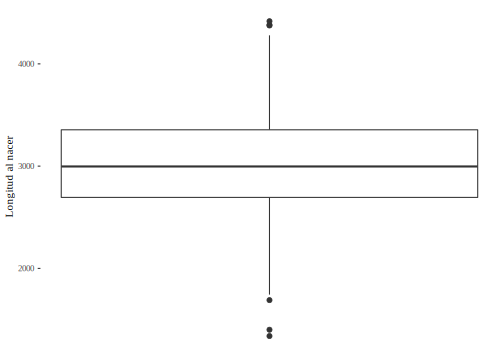
\includegraphics{EstadisticaParaCienciasSocialesConR_files/figure-latex/unnamed-chunk-88-1.pdf}

\hypertarget{medida-de-la-dispersion-cuando-no-hay-distancias}{%
\subsection{Medida de la dispersión cuando no hay distancias}\label{medida-de-la-dispersion-cuando-no-hay-distancias}}

Todo lo indicado hasta el momento acerca de la variabilidad ha
necesitado de la medición de la distancia entre las observaciones: desde el comienzo hablamos de cercanía o lejanía entre los datos. Por lo tanto
estas medidas, desde el recorrido hasta el coeficiente de variación,
solo tienen sentido si la variable es de nivel intervalar o
proporcional. Si la variable tiene nivel nominal u ordinal habrá que
medir su variabilidad de otra forma. En estos casos cambia un poco el
significado de la variabilidad, ya que estaremos en presencia de una
variable más dispersa cuanto más \emph{equitativamente} se distribuya el
total de observaciones entre las distintas categorías. Por ejemplo, si 100 individuos son clasificados según cómo sea su rendimiento en: muy bueno, bueno, regular, insatisfactorio; la distribución tendrá más
dispersión si 25 de ellos se encuentran en cada categoría que si la gran
mayoría está en una sola. La distribución:

\begin{longtable}[]{@{}lcc@{}}
\toprule
Rendimiento & f & f'\tabularnewline
\midrule
\endhead
Muy bueno & 25 & 0.25\tabularnewline
Bueno & 25 & 0.25\tabularnewline
Regular & 25 & 0.25\tabularnewline
Insatisfactorio & 25 & 0.25\tabularnewline
Total & 100 & 1.00\tabularnewline
\bottomrule
\end{longtable}

Tiene más dispersión que esta otra:

\begin{longtable}[]{@{}lcc@{}}
\toprule
Rendimiento & f & f'\tabularnewline
\midrule
\endhead
Muy bueno & 5 & 0.05\tabularnewline
Bueno & 80 & 0.80\tabularnewline
Regular & 5 & 0.05\tabularnewline
Insatisfactorio & 10 & 0.10\tabularnewline
Total & 100 & 1.00\tabularnewline
\bottomrule
\end{longtable}

¿Por qué? Porque en la segunda, los casos están muy concentrados en una categoría (bueno), mientras que en la primera se dispersan entre todas.

Notemos que ahora habrá más dispersión cuanto más parecidas sean las
frecuencias entre sí. Esto puede parecer contradictorio con lo indicado
para variables cuantitativas, pero allí la mayor dispersión viene dada
por la mayor disparidad entre los valores de las variables, que no puede
evaluarse con variables nominales u ordinales.

Esta forma de considerar la dispersión equivale a la idea de
incertidumbre. Supongamos que conocemos que la distribución del
rendimiento es como lo muestra la primera tabla y que debemos ``adivinar''
cuál es el rendimiento de una persona elegida al azar. No tenemos
ninguna razón para creer de manera preferencial que la persona sea de
rendimiento muy bueno, bueno, regular o insatisfactorio; ya que todos
son igualmente posibles. En esta situación, la incertidumbre es
completa. Por el contrario, si supiéramos que la distribución es la que
muestra la segunda tabla, tenderíamos con justa razón a creer que hay
más chances que la persona elegida al azar tenga rendimiento bueno, ya
que es bastante más probable que pertenezca a esa categoría que a otra.
Diremos que aquí tenemos menos incertidumbre.

La medida para expresar de manera sintética esta dispersión es:

\[H\left( x \right) = - \sum_{i = 1}^{k}{{f'}_{i}^{}*log{f'}_{i}^{}}\]

El cálculo consiste en multiplicar cada frecuencia relativa por su
propio logaritmo y sumar para todas las categorías. El resultado de la
sumatoria siempre es negativo, por lo que la fórmula incluye un signo
menos para volverlo positivo. Este coeficiente expresa en un solo número
la magnitud de la dispersión. Cuanto más pequeña sea esta medida, tanto
menos dispersa (o más concentrada) será la distribución de la variable
que se analiza.

Aplicado a las dos tablas de más arriba resulta, para la primera:

\[H\left( x \right) = - (0.25*log0.25 + 0.25*log0.25 + 0.25*log0.25 + 0.25*log0.25) = - \left( - 0.60 \right) = 0.60\]

Y, para la segunda:

\[H\left( x \right) = - (0.05*log0.05 + 0.80*log0.80 + 0.05*log0.05 + 0.10*log0.10) = - \left( - 0.31 \right) = 0.31\]

Así, a la distribución en la que las frecuencias están más concentradas,
es decir la que tiene menor dispersión, le corresponde un menor valor de \(H(x)\).

Cuando la variable tiene solo dos categorías, la proporción de casos en una de ellas es el complemento a uno de la otra, si en una categoría la proporción es \(p\) en la otra será \(1-p\). La máxima concentración se da cuando todos los casos están en una sola categoría, \(p=1\) y \(1-p=0\), allí la dispersión vale cero, porque se trata de una constante: a todos los individuos les corresponde el mismo valor de la variable. La máxima dispersión sucede cuando la distribución entre las dos categorías es equitativa, es decir cuando la mitad de los casos está en cada una: \(p=0.5\) y \(1-p=0.5\).
La medida de esta variabilidad también se llama varianza, pero su cálculo es muy diferente del caso de variables cuantitativas. Para una variable nominal de dos categorías (dicotómica), la varianza es:

\[s^2 = p*(1-p)\]

La desviación estándar es: \[s=\sqrt(p*(1-p))\]
Que alcanza su mínimo en cero cuando todos los casos están en una sola categoría y su máximo en .25 cuando se distribuyen mitad en cada una.

\hypertarget{el-individuo-en-relacion-a-su-grupo}{%
\section{El individuo en relación a su grupo}\label{el-individuo-en-relacion-a-su-grupo}}

Un uso muy frecuente de las medidas que acabamos de ver es que permiten decidir si un \emph{valor particular} está cerca o lejos del promedio, o bien si se sitúa o no en los extremos de una distribución. Un valor particular en este caso se
refiere al valor de la variable en un \emph{caso}, en un \emph{individuo}, por
ejemplo, el puntaje que un sujeto obtiene en una prueba, el ingreso de un hogar, la PBI per cápita de un país. Así formulado
el problema puede parecer muy elemental, porque puede ``verse'' si un
número está cerca o lejos de otro. Si sabemos que una persona tiene dos metros de estatura, no necesitamos hacer cuentas para saber que es alto, más alto que la mayoría de las personas. Sin embargo, en el caso de medidas menos familiares, a veces resulta difícil hacer juicios de distancia sobre valores absolutos. Si un país tiene PBI per cápita de U\$S20000, hace falta conocer más datos para evaluarlo como alto o bajo,

Si sabemos que en una prueba de memoria con un puntaje máximo de 100
puntos, una persona logró 80 puntos, ¿estamos autorizados para decir que obtuvo un puntaje alto? La respuesta es no, porque no sabemos qué
puntajes obtuvieron las demás personas que hicieron la prueba. Si la
media del grupo completo hubiese sido 60 puntos, entonces 80 sería un
valor elevado, pero si la media hubiese sido de 85, entonces el caso que estamos considerando se encontraría por debajo del promedio. Más aún, si el promedio fuese 60 y la mayoría de los evaluados hubiese obtenido puntajes cercanos a 60 (poca variabilidad), entonces el valor 80 podría considerarse como muy elevado. Solo conocer su puntaje individual no nos dice nada acerca de la posición de un sujeto particular. Dos ejemplos:

\begin{itemize}
\item
  Nos informan que un niño obtuvo un puntaje bruto de 85 en
  la escala de desarrollo infantil de Bayley (\citet{Ballot2017}), no tenemos, en principio ningún criterio para decidir si ese puntaje es alto o bajo.
\item
  El Índice de Democracia (\citet{demindex2011}) de un país es 7.5. ¿Dónde se ubica este país en el conjunto de democracias del mundo? ¿Es alto, medio\ldots{}?
\end{itemize}

Para situaciones como éstas, muy frecuentes en evaluaciones
cuantitativas, será necesario conocer cuál es la posición \emph{relativa} que un puntaje ocupa respecto del conjunto completo de observaciones.

Supongamos que se aplica una prueba de ortografía a una muestra de
alumnos de tercer grado y que el promedio de errores es 10
(\(\overline{x} = 10\) errores) y que la desviación estándar es de 4
(\(s = 4\) errores). Si un alumno comete 6 errores (\(x = 6\) errores),
podemos decir que cometió menos errores que el promedio del grupo. El
cálculo de la diferencia entre \(x\) y \(\overline{x}\) da \(-4\) errores
(\(x - \overline{x} = 6 - 10 = - 4\)), este resultado nos informa que este alumno se ubica a 4 errores por debajo del promedio (por debajo queda expresado en el signo menos el resultado). Ésta es una medida concreta, ya que expresa el número de errores que separan al alumno del comportamiento resumido del grupo (expresado en la media); dicho de otra manera, estamos considerando los valores absolutos. Si ahora a esta diferencia la dividimos por la desviación estándar obtenemos \(-1\) (procedente de \(\frac{- 4\ }{\ \ 4\ }\)), que ya no tiene unidades, es un número abstracto. Como la desviación estándar es de 4 puntos y el alumno se encuentra a cuatro puntos de la media, esto equivale a decir que el alumno se encuentra ``a una desviación estándar por debajo del promedio''.

La operación que hemos hecho ha sido la de restar al valor particular
(de ese alumno) la media y dividir el resultado en la desviación
estándar, hemos calculado lo siguiente:

\[\frac{x - \overline{x}}{s}\]

Este número, que como dijimos no tiene unidades, es diferente para cada valor de \(x\), y mide la distancia a la que se encuentra una observación particular (\(x\)) de la media (\(\overline{x}\)), expresada como fracción de la desviación estándar (\(s\)). Decimos que se trata de una medida \emph{estandarizada} del alejamiento que tiene una observación particular del promedio del conjunto de observaciones.

Hemos así expresado la posición del alumno respecto del grupo al que
pertenece de manera relativa, en términos de desviaciones estándar.

La variable que resulta de esta operación se llama \textbf{desvío estándar}, ya que se trata de un desvío (calculado en la diferencia \(x - \overline{x}\)) expresado como cantidad de desviaciones estándar. Se utiliza la letra z para indicarla, así:

\[z = \frac{x - \overline{x}}{s}\]

Debido a que la letra z se utiliza de manera universal para indicar este o \textbf{puntaje z} o \textbf{puntuación z}. Esta
nueva variable tiene media igual a cero y desviación estándar igual a
uno.

Volvamos sobre el ejemplo del número de síntomas en que se basa el
diagnóstico de depresión, cuya media fue de 7 y su desviación estándar
de 1,55.

\begin{longtable}[]{@{}cccc@{}}
\toprule
\begin{minipage}[b]{0.09\columnwidth}\centering
Paciente\strut
\end{minipage} & \begin{minipage}[b]{0.27\columnwidth}\centering
\(x_{i}\) (número de síntomas)\strut
\end{minipage} & \begin{minipage}[b]{0.31\columnwidth}\centering
\(x_{i} - \overline{x}\) (desvíos)\strut
\end{minipage} & \begin{minipage}[b]{0.22\columnwidth}\centering
\(z\) (desvíos estándar)\strut
\end{minipage}\tabularnewline
\midrule
\endhead
\begin{minipage}[t]{0.09\columnwidth}\centering
1\strut
\end{minipage} & \begin{minipage}[t]{0.27\columnwidth}\centering
5\strut
\end{minipage} & \begin{minipage}[t]{0.31\columnwidth}\centering
-2\strut
\end{minipage} & \begin{minipage}[t]{0.22\columnwidth}\centering
-1.29\strut
\end{minipage}\tabularnewline
\begin{minipage}[t]{0.09\columnwidth}\centering
2\strut
\end{minipage} & \begin{minipage}[t]{0.27\columnwidth}\centering
6\strut
\end{minipage} & \begin{minipage}[t]{0.31\columnwidth}\centering
-1\strut
\end{minipage} & \begin{minipage}[t]{0.22\columnwidth}\centering
-0.65\strut
\end{minipage}\tabularnewline
\begin{minipage}[t]{0.09\columnwidth}\centering
3\strut
\end{minipage} & \begin{minipage}[t]{0.27\columnwidth}\centering
6\strut
\end{minipage} & \begin{minipage}[t]{0.31\columnwidth}\centering
-1\strut
\end{minipage} & \begin{minipage}[t]{0.22\columnwidth}\centering
-0.65\strut
\end{minipage}\tabularnewline
\begin{minipage}[t]{0.09\columnwidth}\centering
4\strut
\end{minipage} & \begin{minipage}[t]{0.27\columnwidth}\centering
8\strut
\end{minipage} & \begin{minipage}[t]{0.31\columnwidth}\centering
1\strut
\end{minipage} & \begin{minipage}[t]{0.22\columnwidth}\centering
0.65\strut
\end{minipage}\tabularnewline
\begin{minipage}[t]{0.09\columnwidth}\centering
5\strut
\end{minipage} & \begin{minipage}[t]{0.27\columnwidth}\centering
8\strut
\end{minipage} & \begin{minipage}[t]{0.31\columnwidth}\centering
1\strut
\end{minipage} & \begin{minipage}[t]{0.22\columnwidth}\centering
0.65\strut
\end{minipage}\tabularnewline
\begin{minipage}[t]{0.09\columnwidth}\centering
6\strut
\end{minipage} & \begin{minipage}[t]{0.27\columnwidth}\centering
9\strut
\end{minipage} & \begin{minipage}[t]{0.31\columnwidth}\centering
2\strut
\end{minipage} & \begin{minipage}[t]{0.22\columnwidth}\centering
1.29\strut
\end{minipage}\tabularnewline
\bottomrule
\end{longtable}

La última columna proviene de haber dividido cada desvío en la
desviación estándar (1.55). Los desvíos indican a cuántas unidades de la variable (en este caso \emph{número de síntomas}) se ubica cada caso del promedio. Los desvíos estándar indican a cuántas desviaciones estándar se encuentra cada caso del promedio. El primer paciente está 1.29 desviaciones estándar por debajo del promedio, el tercero está a 0.65 desviaciones estándar por debajo del promedio, etc.

Para variables nominales, se procede de la misma manera, solo cambia el cálculo de la desviación estándar:

Si en un país ``A'' se encuentra que el 12.5\% de los ciudadanos cree que da lo mismo un gobierno autoritario que uno democrático (pregunta P8STGBS de Latinobarómetro) ¿es mucho o poco? Para saberlo necesitamos concer el porcentaje general de esta respuesta en el conjunto de países que se observaron: este valor es, para los países que participan del estudio, 27.6\%. Ahora se sabe que en el país ``A'' la proporción de los que creen que da lo mismo el tipo de gobierno es más baja que en el conjunto de países de la región. ¿Cuánto más baja? Se requiere indicar su posición relativa, y eso se hace en términos de puntaje z. La varianza esta variable se calcula como \(p*(1-p)=.276*(1-.276)=0.1998\) y la desviación estándar como \(\sqrt(0.1998)=.447\). Entonces \(z = \frac{0.125-0.276}{0.447}=-0.34\).

Que indica que ese país esta \emph{levemente} por debajo del conjunto. En los próximos capítulos avanzaremos en el análisis de los puntajes z.

Cuando se trata de variables de nivel ordinal también es posible ubicar de manera relativa cada valor de la variable, aunque no puedan medirse distancias. Es así porque en esas variables podemos calcular percentiles e indicar a qué percentil corresponde cada valor. Antes vimos el modo de señalar gráficamente la ubicación de los percentiles, allí buscamos de identificar el valor de la variable que corresponde, por ejemplo, al percentil 90 ó a cualquier otro. Podemos hacer también el recorrido inverso: dado un valor de la variable ¿a qué percentil corresponde?

Consideremos los siguientes puntajes brutos obtenidos en una prueba
psicológica administrada a una muestra de 310 personas:

\begin{longtable}[]{@{}lccc@{}}
\toprule
x & f & F & F'\tabularnewline
\midrule
\endhead
20-29 & 0 & 0 & 0\tabularnewline
30-39 & 10 & 10 & 0.03\tabularnewline
40-49 & 30 & 40 & 0.13\tabularnewline
50-59 & 50 & 90 & 0.29\tabularnewline
60-69 & 70 & 160 & 0.52\tabularnewline
70-79 & 90 & 250 & 0.81\tabularnewline
80-89 & 40 & 290 & 0.94\tabularnewline
90-99 & 10 & 300 & 0.97\tabularnewline
100-109 & 5 & 305 & 0.98\tabularnewline
110-119 & 5 & 310 & 1\tabularnewline
Total & 310 & &\tabularnewline
\bottomrule
\end{longtable}

Algunos percentiles de esta distribución, por ejemplo, \(P_{20}\), \(P_{60}\) y \(P_{90}\), cuando se piden a R, dan:

\begin{verbatim}
##  P20  P60  P90 
## 54.5 74.5 84.5
\end{verbatim}

Procediendo del mismo modo, se realiza la siguiente correspondencia de puntajes brutos a percentiles:

\begin{longtable}[]{@{}cc@{}}
\toprule
Percentil & X\tabularnewline
\midrule
\endhead
10 & 47.0\tabularnewline
20 & 54.5\tabularnewline
30 & 60.4\tabularnewline
40 & 64.9\tabularnewline
50 & 69.3\tabularnewline
60 & 74.5\tabularnewline
70 & 76.3\tabularnewline
80 & 79.8\tabularnewline
90 & 84.5\tabularnewline
\bottomrule
\end{longtable}

La tabla nos informa sobre los valores de la variable donde se divide
cada 10\% del total de casos. Usando la definición de los percentiles
diremos que:

\begin{itemize}
\tightlist
\item
  El 10\% de los sujetos obtuvo 47 puntos o menos.
\item
  El 20\% obtuvo 54.5 puntos o menos y así para el resto.
\end{itemize}

Con esta información sabemos que si una persona obtuvo 50 puntos, tiene
un puntaje muy bajo, porque supera a menos del 20\% del grupo. O dicho de
otra manera, más del 80\% de las personas alcanzaron puntajes más altos
que él. Por el contrario si alguien obtuvo 88 puntos, tiene un puntaje
muy alto, ya que supera al percentil 90, con lo que menos del 10\% del
grupo lo supera. O bien, él supera a más del 90\%.

De este modo, la construcción de una tabla en la que se indica el valor
de la variable (el puntaje en la prueba) correspondiente a cada
percentil, permite conocer si un puntaje dado se ubica en algún extremo
de la distribución (si es excepcionalmente elevado o bajo) o si es un
valor intermedio.

Estas tablas de correspondencia entre valores absolutos (o puntajes
brutos) y los correspondientes valores relativos pueden también
construirse a partir de los desvíos estándar, para lo que se debe
transformar cada valor observado en su puntuación \(z\). Para el ejemplo
anterior se debe calcular la media y la desviación estándar, que dan:
\(\overline{x} = 68.4\) y \(s = 15.7\). Con esto se indican los puntajes \(z\)
que corresponden a cada puntaje bruto, con la transformación
\(z = \frac{x - \overline{x}}{s}\).

Para la marca de clase del primer puntaje bruto (25), el puntaje z que le corresponde es:

\(z = \frac{25 - 68.4}{15.7} = - 2.8\).

Al repetir esta operación para cada puntaje bruto se obtiene la tabla de correspondencias:

\begin{longtable}[]{@{}cc@{}}
\toprule
Intervalo de puntajes brutos & Puntaje \(z\)\tabularnewline
\midrule
\endhead
20-29 & -2.8\tabularnewline
30-39 & -2.1\tabularnewline
40-49 & -1.5\tabularnewline
50-59 & -0.9\tabularnewline
60-69 & -0.2\tabularnewline
70-79 & 0.4\tabularnewline
80-89 & 1.1\tabularnewline
90-99 & 1.7\tabularnewline
100-109 & 2.3\tabularnewline
110-119 & 3.0\tabularnewline
\bottomrule
\end{longtable}

Una tabla de ese tipo (ya sea construida a partir de los percentiles o bien de los puntajes \(z\)) se conoce como \textbf{baremo} y es absolutamente necesario para cualquier tipo de evaluación psicológica o educativa ya que posibilita decidir en qué lugar se encuentra un sujeto dado, respecto de su grupo de referencia, Esto se requiere porque, por ejemplo, para una prueba de inteligencia, un puntaje que es normal para la edad de 13 años, no lo es para los 16; los puntajes de alguien de 13 años se comparan con los puntajes de otras personas de 13 años. El baremo provee la transformación de puntajes absolutos en puntajes relativos.

\begin{longtable}[]{@{}c@{}}
\toprule
\endhead
\begin{minipage}[t]{0.97\columnwidth}\centering
Un \textbf{baremo} es una tabla de valores transformados que permiten ubicar a un sujeto en relación a su grupo de referencia.\strut
\end{minipage}\tabularnewline
\bottomrule
\end{longtable}

El signo del puntaje z indica si un valor particular está por encima (si es positivo) o por debajo de la media (si negativo). El valor absoluto de z señala cuán lejos o cerca está la observación de la media. Para evaluar esta distancia, contamos con un resultado general, que es válido cualquiera sea la forma de la distribución. Ese resultado establece que a una distancia de hasta un número (\(k\)) determinado de desviaciones estándar se concentra no menos de \(1-\frac{1}{k^2}\) de los casos. Si \(k=2\) este resultado indica que a una distancia de hasta dos desviaciones estándar de la media se concentra por lo menos la fracción \(1-\frac{1}{2^2}=1-\frac{1}{4}=\frac{3}{4}=.75\) de las observaciones. Dicho de otra manera, el intervalo que va desde la media menos dos desviaciones estándar y la media más dos desviaciones estándar contiene al menos al 75\% de los casos. Si \(k=3\), la proporción de casos que allí se encuentra es por lo menos 89\% (que resulta de \(1-\frac{1}{3^2}\).
Ese resultado se conoce como desigualdad de Chebycheff

\[P(|x-media|<k*s)>=1-\frac{1}{k^2}\]

En esta expresión leemos por ahora que la proporción de casos que se encuentran a una distancia de la media menor a \(k\) desviaciones estándar es mayor o igual a uno menos uno sobre \(k\) cuadrado. Cuando se asigna a \(k\) un valor, se puede calcular esa proporción para una distancia concreta a la media.

Si se cumple que la distribución es unimodal y aproximadamente simétrica, esta regla se puede simplificar del siguiente modo:
en el intervalo de \textbf{una} desviación estándar de la media se encuentra aproximadamente el 68\% de los casos, a \textbf{dos} desviaciones el 95 y a \textbf{tres}, el 99\%.

Con estos criterios, podemos evaluar los valores de la variable como pertenecientes al conjunto más frecuente o a los extremos, menos frecuentes, de la distribución. Por ejemplo, si en una distribución simétrica, a un caso le corresponde un puntaje \(z=3\) se trata de un caso excepcionalmente elevado, porque pertenece a una distancia que solo es superada por el .5\% del total de observaciones. Usaremos el criterio de considerar a los casos que estén a menos de dos desviaciones por encima o por debajo ed la media como ``esperables'', porque están en la región de mayor frecuencia. Los casos que estén entre dos y tres desviaciones estándar serán valores ``elevados'' si \(z>0\) y ``bajos'' si \(z<0\). Los casos que se ubican a tres o más desviaciones estándar (\(|z|\geq 3\)) serán considerados ``excepcionalmente'' altos o bajos según el signo de z.

El gráfico siguiente muestra el intervalo de dos desviaciones estándar para una distribución no cumple los supuestos mencionados, a la que se aplica la desigualdad de Chebycheff.

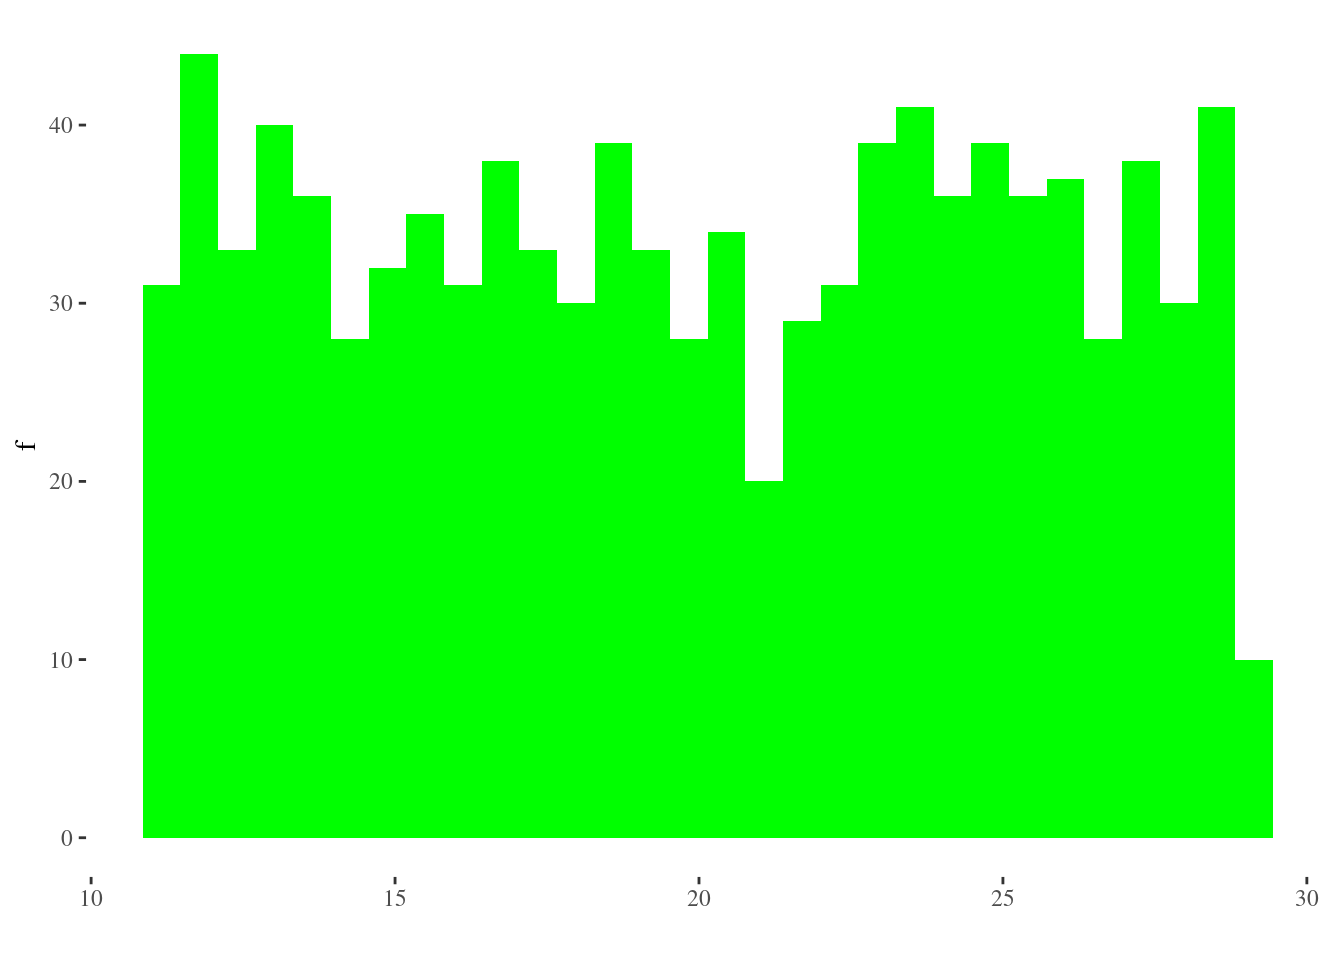
\includegraphics{EstadisticaParaCienciasSocialesConR_files/figure-latex/unnamed-chunk-95-1.pdf}

Mientras que la siguiente distribución es unimodal y aproximadamente simétrica, por lo que es válida la regla empírica.

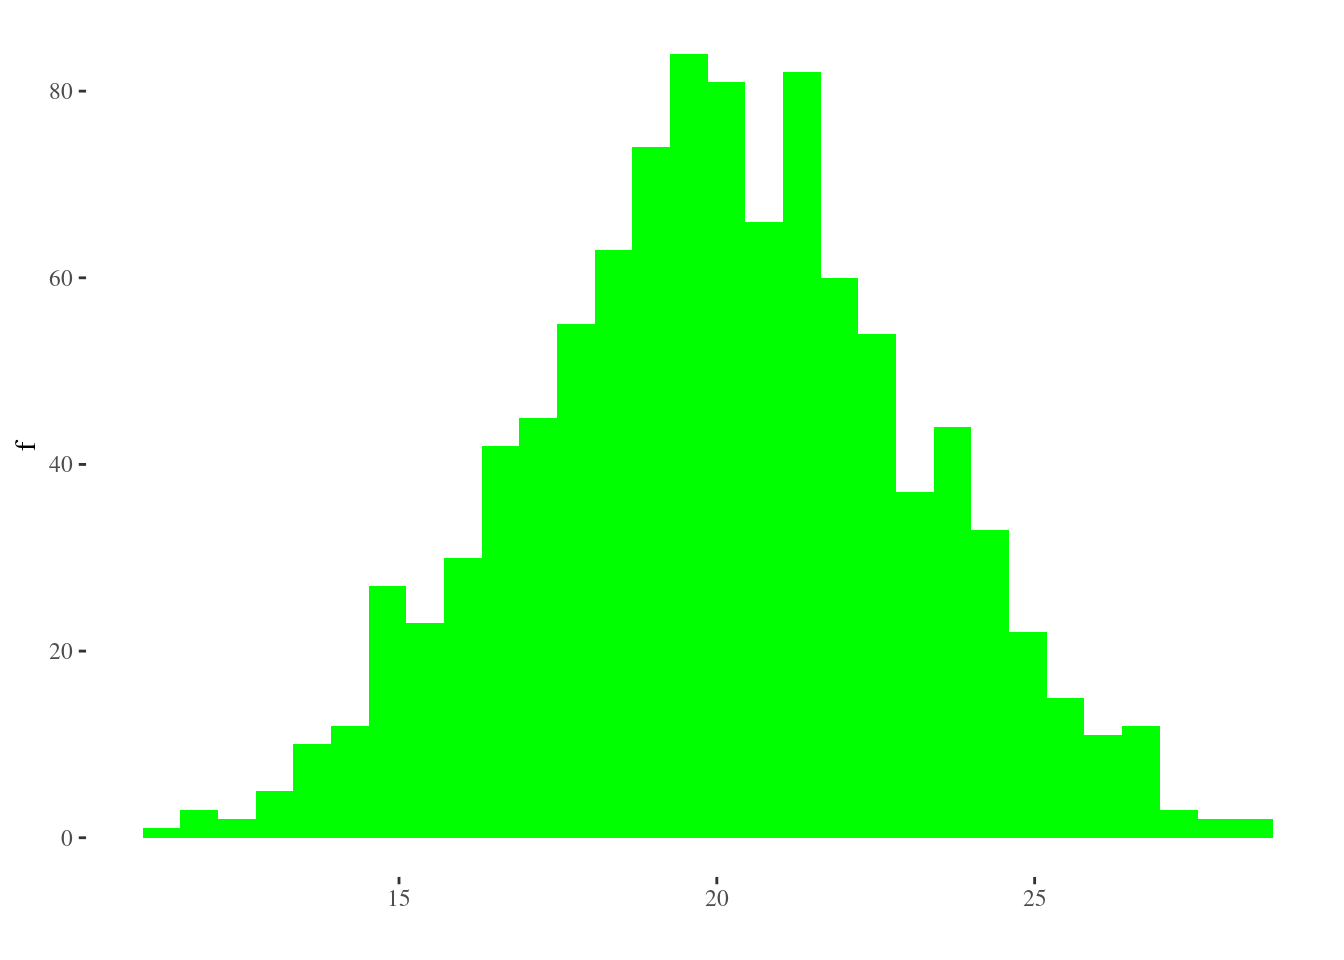
\includegraphics{EstadisticaParaCienciasSocialesConR_files/figure-latex/unnamed-chunk-96-1.pdf}

Volveremos sobre este tema con más detalle cuando tratemos una distribución teórica que se llama distribución normal.

\hypertarget{resumen-de-medidas-descriptivas}{%
\section{Resumen de medidas descriptivas}\label{resumen-de-medidas-descriptivas}}

\hypertarget{medidas-de-posicion-1}{%
\subsection{Medidas de posición}\label{medidas-de-posicion-1}}

\begin{longtable}[]{@{}llc@{}}
\toprule
& & Nivel de medición mínimo requerido\tabularnewline
\midrule
\endhead
Centrales & Modo & Nominal\tabularnewline
& Mediana & Ordinal\tabularnewline
& Media & Intervalar\tabularnewline
No centrales & Cuartiles & Ordinal\tabularnewline
& Quintiles & Ordinal\tabularnewline
& Percentiles & Ordinal\tabularnewline
\bottomrule
\end{longtable}

\hypertarget{medidas-de-dispersion-1}{%
\subsection{Medidas de dispersión}\label{medidas-de-dispersion-1}}

\begin{longtable}[]{@{}llc@{}}
\toprule
& & Nivel de medición mínimo requerido\tabularnewline
\midrule
\endhead
Entre extremos & Recorrido & Intervalar\tabularnewline
Basada en el orden & Amplitud intercuartílica & Intervalar\tabularnewline
Basadas enla media & Varianza & Intervalar\tabularnewline
& Desviación estándar & Intervalar\tabularnewline
& Coeficiente de variación & Intervalar\tabularnewline
De incertidumbre & Coeficiente de incertidumbre & Nominal\tabularnewline
\bottomrule
\end{longtable}

\bibliography{bibliografia.bib}


\end{document}
